%%%%%%%%%%%%%%%%%%%%%%%%%%%%%%%%%%%%%%%%%
%This documentclass loads the packages  %
%            setspace                   %
% and                                   %
%           fancyhdr.                   %
%You may have to                        %
%get these if your TeX distribution     %
%doesn't have them.                     %
%%%%%%%%%%%%%%%%%%%%%%%%%%%%%%%%%%%%%%%%%
\documentclass{aux/ttuthes2007}

%%%%%%%%%%%%%%%%%%%%%%%%%%%%%%%%%%%%%%%%%%%%%%
%Include any other add-on  packages you need:%
%%%%%%%%%%%%%%%%%%%%%%%%%%%%%%%%%%%%%%%%%%%%%%
\usepackage{amsmath,graphicx,bm,mathtools, amssymb}
\allowdisplaybreaks
\usepackage{booktabs} % Required for better horizontal rules in tables
\usepackage{listings} % Required for insertion of code
\usepackage[utf8]{inputenc}
\usepackage[T1]{fontenc}
\usepackage{lmodern}
\usepackage[labelfont=bf,labelsep=period]{caption}
\usepackage{multirow}
\usepackage{textcomp}
\usepackage[colorlinks=true,citecolor=black,linkcolor=black]{hyperref}
\usepackage{afterpage}
\usepackage{pdflscape}
\usepackage{hhline}
\usepackage{enumitem}
\usepackage{hyperref}
\usepackage{bm}
\usepackage[acronyms,toc,nonumberlist,nogroupskip]{glossaries}
\usepackage{datetime}
\usepackage{xstring} % conditionals
\usepackage[dvipsnames]{xcolor}

\newglossary{symbols}{sym}{sbl}{List of Symbols}
\makenoidxglossaries
\glsnoexpandfields

\loadglsentries{aux/gloss.tex}

%%%%%%%%%%%%%%%%%%%%%%%%%%%%%%%%%%
%EDIT  (Running head--  REQUIRED)%
%%%%%%%%%%%%%%%%%%%%%%%%%%%%%%%%%%
\rhead{\small Texas Tech University, \textit{Lucas Ramos Cardoso Tin\^{o}co Cortez}, \monthyeardate\today}	%update your name and graduation date-year here

%%%%%%%%%%%%%%%%%%%%%%%%%%%%%%%%%%%%%%%%%%%%%%%
%Uncomment if the grad school doesn't like the%
%line under the  running head:                %
%%%%%%%%%%%%%%%%%%%%%%%%%%%%%%%%%%%%%%%%%%%%%%%
%\renewcommand{\headrulewidth}{0pt}


%%%%%%%%%%%%%%%%%%%%%%%%%%%%%%%%%%%%%%%%%%%%%%%%%%
%Spacing -- Do you want double or one-and-a-half?%
%%%%%%%%%%%%%%%%%%%%%%%%%%%%%%%%%%%%%%%%%%%%%%%%%%
%\doublespacing
\onehalfspacing
%%%%%%%%%%%%%%%%%%%%%%%%%%%%%%%%%%%%%%%%%%%%%%%%%%%%%%%%%%%%%
%Leave the one you want uncommented.                        %
%In places where single-line-spacing is appropriate         %
%e.g, extended quotations, you can enclose the material     %
%in a singlespacing environment (with \begin{singlespacing} %
% ...  \end{singlespacing}                                  %
%%%%%%%%%%%%%%%%%%%%%%%%%%%%%%%%%%%%%%%%%%%%%%%%%%%%%%%%%%%%%


%%%%%%%%%%%%%%%%%%%%%%%%%%%%%%%%%%%%%%%%%%%%%%%%%%
%Other preamble stuff, e.g., theorem environments%
%or newcommands go here:                         %
% e.g.                                           %
%%%%%%%%%%%%%%%%%%%%%%%%%%%%%%%%%%%%%%%%%%%%%%%%%%
% \newtheorem{theorem}{Theorem}
% \newtheorem{proposition}[theorem]{proposition}
% \newtheorem{question}{Question}
% \newtheorem{conjecture}{Conjecture}
%\newcommand\Set[2]{\left\{\,#1\middle\mid#2\,\right\}}
\newcommand{\bx}{\bm{x}}
\newcommand{\br}{\bm{r}}
\newcommand{\bra}[1]{\ensuremath{\left\langle#1\right\vert}}
\newcommand{\ket}[1]{\ensuremath{\left|#1\right\rangle}}
\newcommand{\braket}[2]{\left< #1 \middle\vert #2 \right>}
\newcommand{\sandwich}[3]{\left< #1 \middle\vert #2 \middle\vert #3 \right>}
%\newcommand{\norm}[1]{\left\lVert #1 \right\rVert}
%\newcommand{\abs}[1]{\lVert #1 \rVert}
\newcommand{\inpr}[1]{\left< #1 \right>}
\newcommand{\s}[1]{\sin\left( #1 \right)}
\newcommand{\ssq}[1]{\sin^2\left( #1 \right)}
\newcommand{\co}[1]{\cos\left( #1 \right)}
\newcommand{\cosq}[1]{\cos^2\left( #1 \right)}
\newcommand{\av}[1]{\left< #1 \right>}
\newcommand{\her}[2]{H_{#1}\left( #2 \right)}
\newcommand{\herv}[1]{H_{\nu}\left( #1 \right)}
\renewcommand{\labelenumi}{\Roman{enumi} -}
\newcommand{\ex}[1]{\exp\left( #1 \right)}
\newcommand{\closepar}{)}
\newcommand{\paren}[1]{\left( #1 \right)}
\newcommand{\ddx}{\frac{d}{dx}}
\newcommand{\ddt}{\frac{d}{dt}}
\newcommand{\pdx}{\frac{\partial}{\partial x}}
\newcommand{\pdt}{\frac{\partial}{\partial t}}
\newcommand{\dd}[1]{\frac{d}{d#1}}
\newcommand{\pd}[1]{\frac{\partial}{\partial #1}}
\newcommand{\fpd}[2]{\frac{\partial #1}{\partial #2}}
\newcommand{\pp}[1]{\frac{\partial \Psi}{\partial #1}}
\newcommand{\kpp}[1]{\frac{\partial \ket\Psi}{\partial #1}}
\newcommand{\bpp}[1]{\frac{\partial \bra\Psi}{\partial #1}}
\newcommand{\kppn}[2]{\frac{\partial^{#2} \ket\Psi}{\partial {#1}^{#2}}}
\newcommand{\bppn}[2]{\frac{\partial^{#2} \bra\Psi}{\partial {#1}^{#2}}}
\newcommand{\kppd}[2]{\frac{\partial^{2} \ket\Psi}{\partial #1 \partial #2}}
\newcommand{\bppd}[2]{\frac{\partial^{2} \bra\Psi}{\partial #1 \partial #2}}
\newcommand{\ddn}[2]{\frac{d^{#1}}{d#2^{#1}}}
\newcommand{\pdn}[2]{\frac{\partial^{#1}}{\partial#2^{#1}}}
%\newcommand{\orb}{N}
%\newcommand{\elec}{n}
\newcommand{\elec}{N}
\newcommand{\nuc}{N_{N}}
\newcommand{\orb}{K}
\newcommand{\Ld}[1]{\hat L_{#1}}
\newcommand{\anio}[1]{a_{\oo{#1}}}
\newcommand{\aniu}[1]{a_{\uo{#1}}}
\newcommand{\anig}[1]{a_{\go{#1}}}
\newcommand{\creo}[1]{a^\dagger_{\oo{#1}}}
\newcommand{\creu}[1]{a^\dagger_{\uo{#1}}}
\newcommand{\creg}[1]{a^\dagger_{\go{#1}}}
\newcommand{\vac}{\ket{vac}}
\newcommand{\anticom}[2]{\left\{ #1, #2 \right\}}
\newcommand{\ind}[1]{{\uo #1 \oo #1}}

\newcommand{\rmatdd}[1]{
		\IfEqCase{#1}{
			{6}{\ensuremath{
	\begin{bmatrix}
		e^{\frac{-i \omega_\ind 0} 2 } & 0 & 0 & 0 \\
		0 & e^{\frac{-i \omega_\ind 0} 2 } & 0 & 0 \\
		0 & 0 & e^{\frac{i \omega_\ind 0} 2 } & 0 \\
		0 & 0 & 0 & e^{\frac{i \omega_\ind 0} 2 }
	\end{bmatrix}
}}
			{5}{\ensuremath{
	\begin{bmatrix}
		e^{\frac{-i \omega_\ind 1} 2 } & 0 & 0 & 0 \\
		0 & e^{\frac{i \omega_\ind 1} 2 } & 0 & 0 \\
		0 & 0 & e^{\frac{-i \omega_\ind 1} 2 } & 0 \\
		0 & 0 & 0 & e^{\frac{i \omega_\ind 1} 2 }
	\end{bmatrix} 
}}
			{4}{\ensuremath{
	\begin{bmatrix}
		\cos\left(\rho_\ind 0\right) & 0 & \sin\left(\rho_\ind 0\right) & 0 \\
		0 & \cos\left(\rho_\ind 0\right) & 0 & -\sin\left(\rho_\ind 0\right) \\
		\sin\left(\rho_\ind 0\right) & 0 & -\cos\left(\rho_\ind 0\right) & 0 \\
		0 & \sin\left(\rho_\ind 0\right) & 0 & \cos\left(\rho_\ind 0\right)
	\end{bmatrix}
}}
			{3}{\ensuremath{
	\begin{bmatrix}
		\cos\left(\rho_\ind 1\right) & -\sin\left(\rho_\ind 1\right) & 0 & 0 \\
		\sin\left(\rho_\ind 1\right) & \cos\left(\rho_\ind 1\right) & 0 & 0 \\
		0 & 0 & -\cos\left(\rho_\ind 1\right) & \sin\left(\rho_\ind 1\right) \\
		0 & 0 & \sin\left(\rho_\ind 1\right) & \cos\left(\rho_\ind 1\right)
	\end{bmatrix}
}}
			{2}{\ensuremath{
	\begin{bmatrix}
		e^{\frac{i \omega_\ind 0} 2 } & 0 & 0 & 0 \\
		0 & e^{\frac{i \omega_\ind 0} 2 } & 0 & 0 \\
		0 & 0 & e^{\frac{-i \omega_\ind 0} 2 } & 0 \\
		0 & 0 & 0 & e^{\frac{-i \omega_\ind 0} 2 }
	\end{bmatrix}
}}
			{1}{\ensuremath{
	\begin{bmatrix}
		e^{\frac{i \omega_\ind 1} 2 } & 0 & 0 & 0 \\
		0 & e^{\frac{-i \omega_\ind 1} 2 } & 0 & 0 \\
		0 & 0 & e^{\frac{i \omega_\ind 1} 2 } & 0 \\
		0 & 0 & 0 & e^{\frac{-i \omega_\ind 1} 2 }
	\end{bmatrix}
}}
		}[\PackageError{r2d}{Undefined option to rmat: #1}{}]
}

\newcommand{\paulid}[1]{
		\IfEqCase{#1}{
			{ii}{I \otimes I}
			{ix}{I \otimes X}
			{iy}{I \otimes Y}
			{iz}{I \otimes Z}
			{xi}{X \otimes I}
			{xx}{X \otimes X}
			{xy}{X \otimes Y}
			{xz}{X \otimes Z}
			{yi}{Y \otimes I}
			{yx}{Y \otimes X}
			{yy}{Y \otimes Y}
			{yz}{Y \otimes Z}
			{zi}{Z \otimes I}
			{zx}{Z \otimes X}
			{zy}{Z \otimes Y}
			{zz}{Z \otimes Z}
		}[\PackageError{p2d}{Undefined option to uo: #1}{}]
}
\newcommand{\uo}[1]{
		\IfEqCase{#1}{
			{0}{\mu}
			{1}{\nu}
			{2}{\xi}
		}[\PackageError{uo}{Undefined option to uo: #1}{}]
}
\newcommand{\oo}[1]{
		\IfEqCase{#1}{
			{0}{\alpha}
			{1}{\beta}
			{2}{\gamma}
		}[\PackageError{unocorb}{Undefined option to unuo: #1}{}]
}
\newcommand{\go}[1]{
		\IfEqCase{#1}{
			{0}{\zeta}
			{1}{\eta}
			{2}{\iota}
			{3}{\kappa}
		}[\PackageError{unocorb}{Undefined option to go: #1}{}]
}
\newcommand{\psiu}[1]{
	\psi_{\uo{#1}}
}
\newcommand{\psio}[1]{
	\psi_{\oo{#1}}
}
\newcommand{\psig}[1]{
	\psi_{\go{#1}}
}

\newcommand{\X}{\begin{bmatrix}	0 & 1 \\ 1 & 0 \end{bmatrix} }
\newcommand{\Y}{\begin{bmatrix}	0 & -i \\ i & 0 \end{bmatrix} }
\newcommand{\Z}{\begin{bmatrix}	1 & 0 \\ 0 & -1 \end{bmatrix} }
\newcommand{\I}{\begin{bmatrix}	1 & 0 \\ 0 & 1 \end{bmatrix} }
\newcommand{\Phase}[1]{\begin{bmatrix} 1 & 0 \\ 0 & e^{i#1} \end{bmatrix} }
\newcommand{\nPhase}[1]{\begin{bmatrix} 1 & 0 \\ 0 & e^{-i#1} \end{bmatrix} }
\newcommand{\II}{\begin{bmatrix}
1 & 0 & 0 & 0 \\
0 & 1 & 0 & 0 \\
 0 & 0 & 1 & 0 \\
0 & 0 & 0 & 1
\end{bmatrix}}
\newcommand{\IX}{ \begin{bmatrix}
0 & 1 & 0 & 0 \\
1 & 0 & 0 & 0 \\
 0 & 0 & 0 & 1 \\
0 & 0 & 1 & 0
\end{bmatrix}}
\newcommand{\IY}{ \begin{bmatrix}
0 & -i & 0 & 0 \\
i & 0 & 0 & 0 \\
 0 & 0 & 0 & -i \\
0 & 0 & i & 0
\end{bmatrix}}
\newcommand{\IZ}{ \begin{bmatrix}
1 & 0 & 0 & 0 \\
0 & -1 & 0 & 0 \\
 0 & 0 & 1 & 0 \\
0 & 0 & 0 & -1
\end{bmatrix}}
\newcommand{\XI}{ \begin{bmatrix}
0 & 0 & 1 & 0 \\
0 & 0 & 0 & 1 \\
 1 & 0 & 0 & 0 \\
0 & 1 & 0 & 0
\end{bmatrix}}
\newcommand{\XX}{ \begin{bmatrix}
0 & 0 & 0 & 1 \\
0 & 0 & 1 & 0 \\
 0 & 1 & 0 & 0 \\
1 & 0 & 0 & 0
\end{bmatrix}}
\newcommand{\XY}{ \begin{bmatrix}
0 & 0 & 0 & -i \\
0 & 0 & i & 0 \\
 0 & -i & 0 & 0 \\
i & 0 & 0 & 0
\end{bmatrix}}
\newcommand{\XZ}{ \begin{bmatrix}
0 & 0 & 1 & 0 \\
0 & 0 & 0 & -1 \\
 1 & 0 & 0 & 0 \\
0 & -1 & 0 & 0
\end{bmatrix}}
\newcommand{\YI}{ \begin{bmatrix}
0 & 0 & -i & 0 \\
0 & 0 & 0 & -i \\
 i & 0 & 0 & 0 \\
0 & i & 0 & 0
\end{bmatrix}}
\newcommand{\YX}{ \begin{bmatrix}
0 & 0 & 0 & -i \\
0 & 0 & -i & 0 \\
 0 & i & 0 & 0 \\
i & 0 & 0 & 0
\end{bmatrix}}
\newcommand{\YY}{ \begin{bmatrix}
0 & 0 & 0 & -1 \\
0 & 0 & 1 & 0 \\
 0 & 1 & 0 & 0 \\
-1 & 0 & 0 & 0
\end{bmatrix}}
\newcommand{\YZ}{ \begin{bmatrix}
0 & 0 & -i & 0 \\
0 & 0 & 0 & i \\
 i & 0 & 0 & 0 \\
0 & -i & 0 & 0
\end{bmatrix}}
\newcommand{\ZI}{ \begin{bmatrix}
1 & 0 & 0 & 0 \\
0 & 1 & 0 & 0 \\
 0 & 0 & -1 & 0 \\
0 & 0 & 0 & -1
\end{bmatrix}}
\newcommand{\ZX}{ \begin{bmatrix}
0 & 1 & 0 & 0 \\
1 & 0 & 0 & 0 \\
 0 & 0 & 0 & -1 \\
0 & 0 & -1 & 0
\end{bmatrix}}
\newcommand{\ZY}{ \begin{bmatrix}
0 & -i & 0 & 0 \\
i & 0 & 0 & 0 \\
 0 & 0 & 0 & i \\
0 & 0 & -i & 0
\end{bmatrix}}
\newcommand{\ZZ}{ \begin{bmatrix}
1 & 0 & 0 & 0 \\
0 & -1 & 0 & 0 \\
 0 & 0 & -1 & 0 \\
0 & 0 & 0 & 1
\end{bmatrix}}
\DeclarePairedDelimiter\norm{\lVert}{\rVert}
\DeclarePairedDelimiter\abs{\lvert}{\rvert}
\newdateformat{monthyeardate}{%
  \monthname[\THEMONTH], \THEYEAR}





\begin{document}

%%%%%%%%%%%%%%%%%%%%%%%%%%%%%%%%%%%%%%%%%%%%%%%%%%%%%%%%
%TITLE PAGE -- Edit the spacing commands after each \\ %
% if necessary                                         %
%%%%%%%%%%%%%%%%%%%%%%%%%%%%%%%%%%%%%%%%%%%%%%%%%%%%%%%%
\begin{titlepage}
\vbox to  \textheight{
\begin{singlespacing}
\begin{center}
New quantum computing techniques applied to chemistry dynamics\\[15pt]  %Edit
by\\[15pt]
Lucas Ramos Cardoso Tin\^oco Cortez, B.S.C.E.\\[15pt]   %Edit to put in your name and whatever degrees you already have
A Dissertation\\[15pt]   % 
In\\[15pt]
Industrial Engineering\\[15pt]
Submitted to the Graduate Faculty\\
of Texas Tech University in\\
Partial Fulfillment of\\
the Requirements for\\
the Degree of\\[15pt]
Doctor of Philosophy in Industrial Engineering\\[30pt]  %Edit (or Master of YYY)
%Approved\\[15pt]
Dr. Bryan Norman\\
Chair of Committee\\[15pt] %Edit
Dr. Ismael Regis de Farias JR\\[15pt] %Edit
Dr. Jorge Alberto Morales \\[15pt] %Edit
Dr. Donping Du\\[15pt] %Edit (add/remove names if you have more or fewer committee members)
Dr. Changxue Xu \\[15pt] %Edit (add/remove names if you have more or fewer committee members)
Dr. Mark Sheridan\\ %Edit (look up the info on the Graduate School's website)
Dean of the Graduate School\\[30pt]
\today      %Edit
\end{center}
\end{singlespacing}
\vfill}
\end{titlepage}
%%%%%%%%%%%%%%%%%%%
%End of title page%
%%%%%%%%%%%%%%%%%%%

%%%%%%%%%%%%%%%%%%%%%%%%%%%%%%%%%%%%%%%%%%%%%%%%%%%%%%%
%Copyright page -- delete or comment out if not needed%
%usage: \copyrightpage{year of appearance}{Name}      %
%%%%%%%%%%%%%%%%%%%%%%%%%%%%%%%%%%%%%%%%%%%%%%%%%%%%%%%
%\copyrightpage{2021}{Lucas Ramos Cardoso Tin\^oco Cortez} %Name should be same as on title page
%%%%%%%%%%%%%%%%%%%%%%%%
%\end of copyright page%
%%%%%%%%%%%%%%%%%%%%%%%%

%%%%%%%%%%%%%%%%%%%%%%%
%Start of frontmatter %
%You need this:       %
%%%%%%%%%%%%%%%%%%%%%%%
\frontmatter


%%%%%%%%%%%%%%%%%%%%%%%%%%%%%
%Acknowledgements           %
%Comment out or delete      %
%if not  wanted             %
%%%%%%%%%%%%%%%%%%%%%%%%%%%%%
%\chapter{\textbf{Acknowledgements}}
%I am thankful that LaTex has made writing my dissertation an easy and painless experience.


%%%%%%%%%%%%%%%%%%%%%%%%%
%End of acknowledgements%
%%%%%%%%%%%%%%%%%%%%%%%%%


%%%%%%%%%%%%%%%%%%%
%Table of Contents%
%%%%%%%%%%%%%%%%%%%
\tableofcontents	%Leave this here (table will auto-update as you write new chapters/subsections/appendix)

%%%%%%%%%%%%%%%%%%%%%%%%%%%%%%%%%%%%%%%%%%%%%%%%%%
%Abstract -- Delete or comment out if not wanted:%
%%%%%%%%%%%%%%%%%%%%%%%%%%%%%%%%%%%%%%%%%%%%%%%%%%
%\chapter{\textbf{Abstract}}

%%%%%%%%%%%%%%%%%
%End of abstract%
%%%%%%%%%%%%%%%%%


%%%%%%%%%%%%%%%%%%%%%%%%%%%%%%%%%%%%%
%List of tables and list of figures %
%Delete or comment out if not needed%
%%%%%%%%%%%%%%%%%%%%%%%%%%%%%%%%%%%%%
%\listoftables	%Leave this here. List will auto-update when you build a new table

\listoffigures	%Leave this here. List will auto-update when you insert new figures
%%%%%%%%%%%%%%%%%%%%%%%%%%%%%%%%%%%%
%End of lists of tables and figures%
%%%%%%%%%%%%%%%%%%%%%%%%%%%%%%%%%%%%



%%%%%%%%%%%%%%%%%%%%%%%%
%MAIN PART OF  DOCUMENT%
%%%%%%%%%%%%%%%%%%%%%%%%

\mainmatter

%TODO: add to introduction what's new work(i.e. section 4)

\chapter{\textbf{Introduction}}

Quantum chemistry \shortcite{szabo,mcweeny} seeks to describe chemical systems in terms of quantum mechanics.
For time-dependent processes (e.g., chemical reactions), that requires the solution of the time-dependent Schrödinger equation \shortcite{szabo,mcweeny}: a partial linear differential equation, second-order in position $r$ and first-order in time $t$, whose unknown is the wavefunction $\ket \Psi = \Psi(r, t)$.
Once the wavefunction is found, all the physical and chemical properties of a system can be directly calculated from it \shortcite{szabo,mcweeny}.

Unfortunately, the solution of the time-dependent Schrödinger equation for many-electron molecules becomes computationally expensive, at worst with a cost scaling exponentially with the system size.
Therefore, different approximations must be introduced.
One approach is to adopt the \gls{tdvp} \shortcite{kramer};
there, a trial wavefunction is optimized with respect to time-dependent parameters with the aim of obtaining a stationary action \shortcite{kramer}. A visualization is provided in figure \ref{fig:TDVP}.

\begin{figure}[ht!]
	\centering
  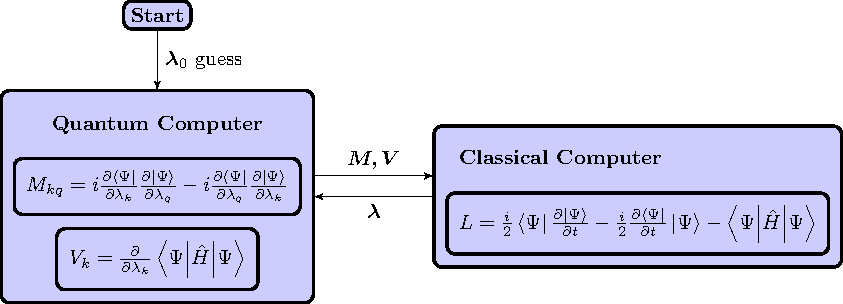
\includegraphics[width=\linewidth]{img/variation_figure.pdf}
  \caption{Visualization of the variational algorithm}
  \label{fig:TDVP}
\end{figure}

The simplest type of trial wavefunction is a \gls{hf} one \shortcite{szabo,mcweeny}:
a single Slater determinant of molecular orbitals (one per electron) that satisfies the Pauli exclusion principle.
However, even with these approximations, finding an optimal trial wavefunction can be exacting on classical (standard) computers.

Fortunately, \gls{qc} \shortcite{nielsen} can offer more efficient algorithms and computers to solve this problem.
As is known, \gls{qc} ultimately expresses all its operations in terms of unitary matrices, such as those of the Pauli gates \shortcite{nielsen}.
In contrast, standard formulations of TDVP and Hartree-Fock theory \shortcite{szabo,mcweeny} avoid a unitary representation.
Years before \gls{qc}, Fukutome \shortcite{fukutome} formulated the time-independent Hartree-Fock theory in terms of unitary Lie groups \shortcite{wybourne} in a purely mathematical context.
In this dissertation, I will extend Fukutome’s unitary group approach to the Hartree-Fock theory to the TDVP framework and develop with it new \gls{qc} algorithms for chemical reactions.
This dissertation is divided into 4 more chapters: In the chapter \ref{chap:background} there'll be an exposition of necessary mathematical and chemical foundations to the work in this dissertation.
Then, in chapter \ref{chap:literature}, some prior work in the area has been highlighted with a brief explanation of how they're relevant to this work.
Also, some book recommendations for further study or from which some formulas and theorems were used in this paper.

Chapter \ref{chap:methodology} is where my work is introduced and explained. Finally, chapter \ref{chap:results} highlights the importance of this work and suggests some directions for further study.

\chapter{\textbf{Background}}\label{chap:background}

The first step to be achieved here is to obtain a starting wavefunction state $\ket\Psi$ of the system for the \gls{tdvp} in the context of quantum computing. 
To do so, we first need to explore the second quantization formulation of quantum chemistry. 
This will yield us the creation and annihilation operations necessary to manipulate wavefunctions.
These operators generate a Lie Algebra, and Fukutome's work \shortcite{fukutome} uses those algebras to relate all possible Slater Determinant states (wavefunctions for our electron system) given a starting reference state $\ket\Psi$.

\section {\textbf{Second Quantization in Quantum Chemistry}}

%\cite{ref1} \cite{szabo}
%{ref3} = FUKUTOME
Let $\elec$ be the number of electrons in our system and $\orb$ be the total number of available orthonormal spin orbitals being considered for our electrons.
Note that since every electron requires an orbital, $\orb \geq \elec$.
Let 
$\{\oo{0}, \oo{1}, \oo{2}, \ldots\}$
index our $\elec$ occupied orbitals (also known as hole orbitals), 
$\{\uo{0},\uo{1},\uo{2}, \ldots\}$ 
index  our $\orb - \elec$ unoccupied orbitals (also called particle orbitals) and 
$\{\go{0}, \go{1}, \go{2}, \go{3}, \ldots\}$
index our $\orb$ orbitals in general.
Let $\nuc$ be the number of nuclei in our system.

To simplify our system, we shall consider that the nuclei are at rest to calculate the electron dynamics. Therefore, our formulation consists of $\orb$ orthonormal electronic spin orbitals $\psig 0(\mathbf{x}_1), \go{0} = 1, 2, \ldots, \orb$ with $\orb \geq \elec$, where $\bx_1 = \paren{\br_1, \sigma_1}$ with $\br_1$ denoting the spatial coordinate and $\sigma_1$ denoting the spin coordinate.

We also have the second-quantization creation operators $\creg{0}$, annihilation operators $\anig{0}$ and vacuum state $\vac$ for our electrons.
In short, creation and annihilation are inverse operations and they work as follows:
\begin{equation*}
\begin{split}
	\creg 0 \vac &= \ket{\psig 0} \\
	\creg 0 \creg 1 \vac &= \creg 0 \ket{\psig 1} = \ket{\psig 0\psig 1} \\
	\creg 1 \creg 0 \vac &= \creg 1 \ket{\psig 0} = \ket{\psig 1\psig 0} = - \ket{\psig 0\psig 1} = -\creg 0 \creg 1 \vac\\
	\anig 0 \vac &= 0 \\
	\anig 0 \ket{\psig 0}  &= \vac 
\end{split}
\end{equation*}
%Possibly expose what operators do here
The operators also satisfy these anti-commutation relationships:
$$\anticom{\creg 0}{\anig 1} = \delta_{\go 0 \go 1}; \anticom{\creg 0}{\creg 1} = \anticom{\anig 0}{\anig 1} = 0$$

Using these operators, we can write the reference Slater determinant state $\ket \Psi$ with occupied spin orbitals $\psio 0, \psio 1, \ldots \psi_\elec$ as:

\begin{equation*}
\begin{split}
	\ket\Psi 
	= \creo 0 \creo 1 \ldots a^\dagger_{\elec} \vac 
	= \ket {\psio 0 \psio 1 \ldots \psi_\elec} 
	= \det \left[\psio 0(\bx_i)\right]
\end{split}
\end{equation*}

We can then denote the excited slater determinants as:

$$
	\ket {\Psi_{\oo 0}^{\uo 0}}
	= \creu 0 \anio 0 \ket\Psi 
	= \ket{\psiu 0 \psio 1 \ldots \psi_\elec} 
$$
$$
	\ket {\Psi_{\oo 0 \oo 1}^{\uo 0 \uo 1}}
	= \creu 1 \anio 1 \creu 0 \anio 0 \ket\Psi 
	= \ket{\psiu 0 \psiu 1 \psio 2 \ldots \psi_\elec} 
$$

The Hamiltonian for the electrons in the system, using second quantization and atomic units is then:
\begin{equation*}
\begin{split}
	\hat H_e = \sum_{\go 0, \go 1}h_{\go 0 \go 1}\creg 0 \anig 1 + 
	\frac 1 4 \sum_{\go 0, \go 1, \go 2, \go 3} \sandwich{\go 0 \go 1}{}{\go 2 \go 3}\creg 0 \creg 1 \anig 2 \anig 3
\end{split}
\end{equation*}
where the one-electron integral $h_{\go 0 \go 1}$ and the two electron integral $\sandwich{\go 0 \go 1}{}{\go 2 \go 3}$ are:
\begin{equation*}
\begin{split}
	h_{\go 0 \go 1} 
	&= \sandwich {\go 0} {h} {\go 1} 
	= \int\psig 0^*(\bx_1)h(\br_1)\psig 1(\bx_1)d\bx_1 \\
	\sandwich{\go 0 \go 1}{}{\go 2 \go 3}
	&= \braket{\go 0 \go 1}{\go 2 \go 3} - \braket{\go 0 \go 1}{\go 3 \go 2}\\
	\braket{\go 0 \go 1}{\go 2 \go 3}
	&= \iint
	\psig 0^*(\bx_1)\psig 2(\bx_1) 
	\frac 1 {r_{12}}
	\psig 1^*(\bx_2)\psig 3(\bx_2) 
	d\bx_1 d\bx_2 
\end{split}
\end{equation*}
Finally, $h(\br_1)$ is the one-electron hamiltonian and $\frac 1 {r_{12}}$ is the Coulumb repulsion operator.

\section{\textbf{Lie Algebras}}

With our creation and annihilation operators defined in the previous section, we can take a look at the groups generated by these operators.
We are denoting the $x$-dimensional unitary groups as $U(x)$, where we are mostly concerned with $U(\orb)$, $U(\elec)$ and $U(\orb - \elec)$.
Within $U(\orb)$, we are also concerned with the Lie Algebra generated by the operators 
${\creg 1 \anig 0}$.
Within $U(\elec)$ and $U(\orb - \elec)$ respectively, we are concerned with the associated Lie algebras generated by the operators 
${\creo 1 \anio 0}$,
${\creu 1 \aniu 0}$,
${\creo 0 \aniu 0}$
and 
${\creu 0 \anio 0}$,
which are subalgebras of the $U(\orb)$ Lie algebra.

Our set of orthonormal spin-orbitals $\psig 0 $ is not unique and there are unitary (A matrix $A$ is unitary if $A^\dagger A = AA^\dagger = \bm{1}$) matrices $\bm{u} = \paren{u_{\go 0 \go 1}}$ that transform it into a new set of orthonormal spin-orbitals $\phi_{\go 0}$:
\begin{equation}\label{eq:neworbs}
\begin{split}
	\phi_{\go 0} 
	&= \sum_{\go 1} \psig 1 u_{\go 1 \go 0} \implies \phi 
	= \psi \cdot \bm u\\
	\bm {u}
	&=\paren{u_{\go 0 \go 1}};
	u_{\go 0 \go 1} = \braket {\psig 1}{ \phi_{\go 0}}
\end{split}
\end{equation}

Since $\bm{u}$ is invertible, so is the transformation of our spin-orbitals. The orthonormality is also preserved by the unitarity of $\bm{u}$.
The creation $b_{\go 0}^\dagger$ and annihilation $b_{\go 0}$ operators associated with the new orbitals $\phi_{\go 0}$ are similarly related to the operators associated with the orbitals $\psig 0$:
\[
	b_{\go 0}^\dagger = \sum_{\go 1} \creg 1 u_{\go 1 \go 0} = \paren{\bm{a}^\dagger\bm{u}}_{\go 0} \implies \bm{b}^\dagger = \bm{a}^\dagger \bm{u}
\]
The reference Slater determinant state (one of the wavefunctions that describe the electrons in our system) $\ket\Phi$ in terms of the occupied spin-orbitals $\phi_{\oo 0}, \phi_{\oo 1}, \ldots \phi_\elec$ is
\[
	\ket \Phi 
	= b_{\oo 0}^\dagger b_{\oo 1}^\dagger \ldots b_\elec^\dagger \vac
	= \ket{\phi_{\oo 0} \phi_{\oo 1} \ldots \phi_\elec}
	= \det \left[\phi_{\oo 0}(\bx_i)\right]
\]

\section {\textbf{Fukutome Unitary Approach to Hartree-Fock Theory}}
%\cite{wybourne} \cite{raczka}

We now know more about the Lie Algebra in $U(\orb)$ generated by the creation and annihilation operators, but this set is too large.
We can reduce our search space by looking at some important subalgebras generated by subsets of the creation and annihilation operators, namely the set of operators that don't mix our occupied and unoccupied orbitals (they act in 2 occupied orbitals or in 2 unoccupied orbitals, so they don't change the number of electrons in either) and the set of operators that do mix occupied and unoccupied orbitals (which either move an electron from occupied to unoccupied orbitals or vice-versa).

Investigating these will show we can focus our attention in one of these subsets of operators and ultimately reduce the amount of Slater determinants we need to consider, and with that, the number of variables that describe our system.

Fukutome \shortcite{fukutome} formulated the \gls{hf} theory in terms of the unitary Lie group $U(\orb)$. First consider the set of $\orb^2$ paired operators $\creg 1 \anig 0$. These are generators of the Lie algebra $U(\orb)$ with commutation relationships (Lie products):
\begin{equation}\label{eq:lieprod}
	\left[ \creg 0 \anig 1, \creg2 \anig 3 \right]
	= \delta_{\go 1 \go 2}\creg 0 \anig 3 - \delta_{\go 0 \go 3} \creg 2 \anig 1
\end{equation}
These generators give rise to unitary transformations $\hat U(\bm{\gamma})$ that are members of the associated unitary Lie group $U(\orb)$
\begin{align*}
	\hat{U}(\bm \gamma) = \exp\paren{\hat\Gamma(\bm \gamma)} = \exp\paren{\sum_{\go 0, \go 1}\gamma_{\go 0 \go 1} \creg 0 \anig 1 }
\end{align*}

Where the matrix $\bm \gamma = \paren{\gamma_{\go 0 \go 1}} \in \mathbb{C}^{\orb\times\orb}$ is anti-Hermitian($\gamma_{\go 0 \go 1} = -\gamma_{\go 1 \go 0}^*$).
Its elements are $\orb^2$ complex parameters that define the transformations $\hat U(\bm \gamma)$.
These parameters are not independant since they satisfy the anti-Hermitian condition, but taking the real and imaginary parts of each $\gamma_{\go 0 \go 1}$ and appealing to the unitary property, it is easy to prove that the transformations $\hat U(\bm \gamma)$ have $\orb^2$ real independant parameters.
Like the $\hat U(\bm \gamma)$, the unitary matrices $\bm u$ belonging to the unitary Lie group $U(\orb)$ are defined as:

\begin{equation}\label{LieMatrices}
	\bm u = \exp(\bm \gamma), \bm\gamma = (\gamma_{\go 0 \go 1}) \in \mathbb{C}^{\orb\times\orb}
\end{equation}
The transformations $\hat U(\bm \gamma)$ and the matrices $\bm u$ constitute operator and matrix realizations of the unitary Lie group $U(\orb)$, respectively. These realizations are isomorphic so that:

\[
	\hat U(\bm{\gamma''}) = \hat U(\bm{\gamma'}) \cdot \hat U(\bm{\gamma}) \sim \bm{u''} = \bm{u'} \cdot \bm u
\]
Fukutome expresses this isomorphism more compactly by reparametrizing $\hat U(\bm \gamma)$ in terms of $\bm u$ via \ref{LieMatrices} and write

\[
	\hat U(\bm{u''}) = \hat U(\bm{u'u}) 
	= \hat U(\bm{u'}) \hat U (\bm{u}) 
\]
By taking the matrix $\bm u$ as that of the spin-orbits transformation in \ref{eq:neworbs}, the action of $\hat U(\bm \gamma)$ on the reference Slater determinant $\ket \Psi$ is:

\begin{equation}\label{eq:orbsequiv}
\begin{split}
	\hat U(\bm \gamma)\ket\Psi
	&= \hat U \left[\bm u = \exp(\bm \gamma) \right] \creo 0 \creo 1 \ldots a_\elec^\dagger\vac\\
	&= \paren{a^\dagger \bm u}_{\oo 0} 
	\paren{a^\dagger \bm u}_{\oo 1} \ldots 
	\paren{a^\dagger \bm u}_\elec \vac
	= \ket\Phi
\end{split}
\end{equation}
which can be proven by successively applying the relationship 
\[
	{\hat U(\bm \gamma) \creg 0  = \sum_{\go 1} \creg 1 u_{\go 1 \go 0} \hat U(\bm \gamma)}
\]
to the occupied creation operators in the second term of \ref{eq:orbsequiv}. That equation states that given a Slater determinant state $\ket\Psi$, all other Slater determinant states $\ket\Phi$ which aren't orthogonal to $\ket \Psi$ can be generated by a unitary transformation $\hat U(\bm \gamma)$ on $\ket\Psi$. This indicates that the Slater determinant states $\ket\Phi$ can be defined in terms of the parameter $\bm \gamma = \paren{\gamma_{\go 0 \go 1}}$. These parameters are very useful in the context of the \gls{tdvp} as we will discuss in Section \ref{sec:tdvp}

Since many particle-hole pair operators $\creg 0 \anig 1$ do not commute, as seen in \ref{eq:lieprod}, it is in most cases impossible to factorize the many-complex-parameter unitary operators $\hat U(\bm \gamma)$ completely into one-complex-parameter unitary operators 
$\hat U(\theta_{\go 0 \go 1}) = \exp\paren{\theta_{\go 0 \go 1}\creg 0 \anig 1 - \theta_{\go 0 \go 1}^*\anig 1 \creg 0}$
This is regrettable because the application of $\hat U(\bm \gamma)$ may be cumbersome for large $\orb$.
Fortunately, different types of partial factorizations of $\hat U(\bm \gamma)$ are possible.
Fukutome factorization starts by assorting the pair operators $\creg 0 \anig 1$ into hole-hole pair $\creo 0 \anio 1$, particle-particle pair $\creu 0 \aniu 1$ and particle-hole/hole-particle $\creu 0 \anio 0 / \creo 0 \aniu 0$ pair operators. 
We first notice that from Eq. \ref{eq:lieprod} that the $\creo 0 \anio 1$ and $\creu 0 \aniu 1$
operators are generators of the Lie algebras $U( \elec )$ and $U ( \orb - \elec )$, respectively. Furthermore, the
hole-hole and particle-particle pair operators commute $\left[\creo 0 \anio 1, \creu 0 \aniu 1\right] = 0 \implies {U(\elec) \cap U(\orb - \elec) = 0}$, ${U(\orb) = U(\elec)\oplus_d U(\orb - \elec)} $ where $\oplus_d$ denotes ordinary direct sum (to be distinguished from the Kronecker sum denoted by $\oplus_k$). Based on these observations, we can define the following anti-Hermitian operators:

\begin{equation*}
\begin{split}
	\Gamma &= \Xi + \Lambda \\
	\Xi &= \Xi_{\oo 0 \oo 1} + \Xi_{\uo 0 \uo 1} \\
	\Xi_{\oo 0 \oo 1} &= \sum_{\oo 0 , \oo 1}\xi_{\oo{0}\oo{1}} a_{\oo 0}^\dagger a_{\oo 1},\ 
	\xi_{\oo{0}\oo{1}} = -\xi_{\oo{1}\oo{0}}^* \\
	\Xi_{\uo 0 \uo 1} &= \sum_{\uo 0, \uo 1} \overline\xi_{\uo{0}\uo{1}} a_{\uo 0}^\dagger a_{\uo 1}, \ 
	\overline\xi_{\uo{0}\uo{1}} = -\overline\xi_{\uo{1}\uo{0}}^* \\
	\left[\Xi_{\oo 0 \oo 1}, \Xi_{\uo 0 \uo 1}\right] &= 0 \\
	\Lambda &= \paren{\sum_{\uo 0, \oo 0}
	\lambda_{\uo 0 \oo 0} a_{\uo 0}^\dagger a_{\oo 0} 
	- \lambda_{\uo 0 \oo 0 }^* a_{\oo 0}^\dagger a_{\uo 0}} 
\end{split}
\end{equation*}
It is immediate that a unitary operator having $\Xi = \Xi_{\oo 0 \oo 1} + \Xi_{\uo 0 \uo 1}$ trivially factorizes as 
$\exp\paren{\Xi} = \exp\paren{\Xi_{\oo 0 \oo 1} + \Xi_{\uo 0 \uo 1}} = \exp\paren{\Xi_{\oo 0 \oo 1}} \cdot \exp\paren{\Xi_{\uo 0 \uo 1}}$
However, Fukutome demonstrated a non-trivial factorization of the unitary transformations $\hat U(\bm u) = \exp\paren\Gamma$ as:
\begin{equation*}
\begin{split}
	&\hat U(\bm u) = \hat U(\bm u_\lambda)\hat U(\bm u_\xi) \iff
	\exp\paren\Gamma 
	= \exp\paren\Lambda \cdot \exp\paren\Xi \sim \bm u 
	= \bm u_\lambda \bm u_\xi \\
	&\hat U(\bm \xi) = \hat U(\bm u_\xi) = \exp\paren\Xi \\
	&\hat U(\bm \lambda) = \hat U(\bm u_\lambda) = \exp\paren\Lambda 
\end{split}
\end{equation*}
Above, the matrices $\bm u_\xi \in \mathbb{C}^{\orb \times \orb}$ are in terms of matrices 
$\bm w \in \mathbb{C}^{\elec \times \elec}$
and
$\overline{\bm w} \in \mathbb{C}^{\paren{\orb - \elec} \times \paren{\orb - \elec}}$ as:
\begin{equation*}
\begin{split}
	\bm u_\xi &= \bm w \oplus_d \overline{\bm w} 
	= \begin{bmatrix}\bm w & \bm 0_{\elec \times \paren{\orb - \elec}} \\ \bm 0_{\paren{\orb - \elec} \times \elec} & \overline {\bm w} \end{bmatrix}	
	\subset U(\orb) \\
	\bm w &= \exp\paren{ \bm \xi } \subset U(\elec) \\
	\bm \xi  &= (\xi_{\oo 0 \oo 1})_{\elec \times \elec} \\
	\overline {\bm w} &= \exp\paren{\overline {\bm \xi} } \subset U(\orb - \elec) \\
	\overline{ \bm \xi } &= (\overline\xi_{\uo 0 \uo 1})_{(\orb - \elec)\times(\orb - \elec)} 
\end{split}
\end{equation*}
In addition, the matrices $\bm u_\lambda \in \mathbb{C}^{\orb \times \orb}$ are
\begin{equation*}
\begin{split}
	\bm u_\lambda &= \begin{bmatrix}\bm C(\lambda) & -\bm S^\dagger(\lambda) \\ \bm S(\lambda) & \tilde {\bm C}(\lambda)\end{bmatrix} \subset U(\orb) \\
	\bm \lambda &= (\lambda_{\uo 0 \oo 0})_{(\orb - \elec)\times \elec} \in \mathbb{C}^{\paren{\orb - \elec} \times \elec} \\
	\bm S(\bm \lambda) &= \sum_{k=0}^\infty \frac{(-1)^k}{(2k + 1)!}\bm \lambda(\bm \lambda^\dagger\bm \lambda)^k \in \mathbb{C}^{\paren{\orb - \elec} \times \elec}\\
	\bm C(\bm \lambda) &= \bm I_\elec + \sum_{k=1}^\infty \frac{(-1)^k}{(2k)!}(\bm \lambda^\dagger\bm \lambda)^k \in \mathbb{C}^{\elec \times \elec}\\
	\tilde {\bm C}(\bm \lambda) &= \bm I_{(\orb - \elec)} + \sum_{k=1}^\infty \frac{(-1)^k}{(2k)!}(\bm \lambda\bm \lambda^\dagger)^k \in \mathbb{C}^{\paren{\orb - \elec} \times \paren{\orb - \elec}}
\end{split}
\end{equation*}

The matrix function $\bm S(\bm \lambda)$ is a generalization of the sine function while the matrixes $\bm C(\bm \lambda)$ and $\tilde {\bm C}(\bm \lambda)$ are generalizations of the cosine function. They also satisfy generalizations of the trigonometric relationships, such as:

\begin{equation*}
\begin{split}
	&\bm C^2(\bm \lambda) + \bm S^\dagger(\bm \lambda)\bm S(\bm \lambda) = \bm I_{\elec} \\
	&\tilde{\bm C}^2(\bm \lambda) + \bm S(\bm \lambda)\bm S^\dagger(\bm \lambda) = \bm I_{\paren{\orb - \elec}} \\
	&\bm S(\bm \lambda)\bm C(\bm \lambda) = \tilde{\bm C}(\bm \lambda)\bm S(\bm \lambda)
\end{split}
\end{equation*}

The matrices $\bm u_\xi$ and $\bm u_\lambda$ form two unitary subgroups with 
$\elec^2 + \paren{\orb - \elec}^2$ 
and 
$2\elec\paren{\orb - \elec}$
real parameters, respectively, within the Lie Group 
$U(\orb)$. $\bm u \in U(\orb)$ has $\orb^2$ real parameters:
$\elec^2 + \paren{\orb - \elec}^2 + 2\elec\paren{\orb - \elec} = \orb^2$
Also, all 
$\bm u_\xi, \bm u_\lambda, \bm u \in \mathbb{C}^{\orb\times\orb}$.

The actions of the matrices $\bm w, \overline{\bm w}$ and $\bm u_\xi = \bm w \oplus_d \overline{\bm w}$ on the spin orbitals $\psig 0$ are:
\begin{equation*}
\begin{split}
	&\phi_{\oo 0} = 
	\sum_{\oo 1}\psio 1 w_{\oo 1 \oo 0} \implies \phi^{\oo 0} = \psi^{\oo 0} \bm w \\
	&\phi_{\uo 0} = 
	\sum_{\uo 1}\psiu 1 \overline w_{\uo 1 \uo 0} \implies \phi^{\uo 0} = \psi^{\uo 0} \overline{\bm w} \\
	&\phi_{\go 0} = 
	\sum_{\go 1}\psio 1 \paren{u_\xi}_{\go 1 \go 2} \implies \phi = \psi \bm u_{\xi} 
\end{split}
\end{equation*}
That is:
\begin{equation*}
\begin{split}
	&\paren{\phi_1 \ldots \phi_{\oo 0} \ldots \phi_\elec}
	= \paren{\psi_1 \ldots \psi_{\oo 0} \ldots \psi_\elec} \bm w\\
	&\paren{\phi_{N + 1} \ldots \phi_{\uo 0} \ldots \phi_\orb}
	= \paren{\psi_{N +1} \ldots \psi_{\uo 0} \ldots \psi_\orb} \bm w\\
	&\paren{\phi^{\oo 0}, \phi^{\uo 0}}
	= \paren{\psi^{\oo 0}, \psi^{\uo 0}}
	\begin{pmatrix}\bm w & \bm 0 \\ \bm 0 & \overline {\bm w} \end{pmatrix} 
\end{split}
\end{equation*}
$\bm w$ transforms occupied spin-orbitals into occupied spin-orbitals while $\overline{\bm w}$ transforms unoccupied spin-orbitals amongst themselves and $\bm u_\xi$ makes both transformations at once.
Meanwhile, the action of $\bm u_\lambda$ on the spin-orbitals $\psi_{\go 0}$ is:

\begin{equation*}
\begin{split}
	&\phi_{\oo 0} 
	= \sum_{\oo 1} \psio 1 \left[\bm C(\bm \lambda)\right]_{\oo 1 \oo 0}
	+ \sum_{\uo 0} \psiu 0 \left[\bm S(\bm \lambda)\right]_{\uo 0 \oo 0} \\
	&\phi_{\uo 0} 
	= \sum_{\uo 1} \psiu 1 \left[\tilde{\bm C}(\bm \lambda)\right]_{\uo 1 \uo 0}
	- \sum_{\oo 0} \psio 0 \left[\bm S^\dagger(\bm \lambda)\right]_{\oo 0 \uo 0} \\
	&\paren{\phi^{\oo 0}, \phi^{\uo 0}}
	= \paren{\psi^{\oo 0}, \psi^{\uo 0}}
	\begin{bmatrix}\bm C(\bm \lambda) & -\bm S^\dagger(\bm \lambda) \\ \bm S(\bm \lambda) & \tilde {\bm C}(\bm \lambda)\end{bmatrix} 
\end{split}
\end{equation*}
The actions of the corresponding unitary transformations 
$\hat U(\bm u_\xi)$, $\hat U(\bm u_\lambda)$ and 
\\
$\hat U(\bm u) 
= {\hat U(\bm u_\xi) \hat U(\bm u_\lambda)}$
on the reference Slater determinant state $\ket\Psi$ are:
\begin{equation*}
\begin{split}
	\hat U(\bm u_\xi) \ket\Psi
	&= \paren{a^\dagger \bm u}_1\ldots
	\paren{a^\dagger \bm u}_{\oo 0}\ldots
	\paren{a^\dagger \bm u}_\elec \vac 
	= \det(\bm w)\ket\Psi \sim \ket \Psi\\
	%Second Line
	\hat U(\bm u_\lambda) \ket\Psi
	&= \prod_{\oo 0 = 1}^\elec
	\left\{\creo 1 [\bm C(\bm \lambda)]_{\oo 1 \oo 0} 
	+ \creu 0 [\bm S(\bm \lambda)]_{\uo 0 \oo 0} \right\}\vac \\
	&= \ket{\ldots \left\{\psio 1 [\bm C(\bm \lambda)]_{\oo 1 \oo 0} 
	+ \psiu 0 [\bm S(\bm \lambda)]_{\uo 0 \oo 0} \right\} \ldots} \\
	&= \ket{\ldots \phi_{\oo 0} \ldots} 
	= \ket\Phi \\
	\hat U(\bm u)\ket\Psi
	&= \hat U(\bm u_\lambda) \hat U(\bm u_\xi)\ket\Psi
	=\det(\bm w)\ket\Phi \sim \ket \Phi
\end{split}
\end{equation*}
Specifically, $\hat U(\bm u_\xi)$ combines occupied spin-orbitals $\psio 0$ among themselves, transforming $\ket \Psi$ into equivalent states $\det (\bm w) \ket \Psi$, where $\det (\bm w) = \exp(i \oo 0), \oo 0 \in \mathbb{R}$, because $\bm w$ is unitary.
In contrast, $\hat U(\bm u_\lambda)$ combines occupied $\psio 0$ and unoccupied $\psiu 0$ spin-orbitals, which transforms $\ket \Psi$ into non-equivalent states $\ket \Phi$.
Therefore, we can ommit $\hat U(\bm u_\xi)$ from $\hat U(\bm u)$.
In this way, we can reduce the original $\orb^2$ real parameters of $\hat U(\bm u)$ to the $2\elec(\orb - \elec)$ real parameters of $\hat U(\bm u_\lambda)$ as they are the minimum, non-reduntant real parameters to generate all the possible Slater determinant states $\ket\Phi$ that aren't orthogonal to the reference state $\ket\Psi$.
According to Thouless theorem \cite{thouless}, the states $\ket\Phi$ can be rewritten as:

\begin{equation}\label{eq:thouless}
\begin{split}
	\ket\Phi 
	= \overline N \prod_{\oo 0 = 1}^\elec \paren{\creo 0 + \creu 0 z_\ind 0}\vac 
	= \overline N \exp \paren{ \sum_{\uo 0, \oo 0} z_\ind 0 \creu 0 \anio 0} \ket\Psi
	= \overline N \ket{\bm z}
\end{split}
\end{equation}
Where the new $\orb(\orb - \elec)$ complex-valued parameters $z_\ind 0$ are
\begin{equation*}
\begin{split}
	&z_\ind 0 
	= \left[ \bm S(\bm \lambda)\bm C^{-1}(\bm \lambda)\right] \\
	&\bm z = (z_\ind 0)
\end{split}
\end{equation*}
and the normalization constant $\overline N$ is
\begin{equation*}
\begin{split}
	\overline N
	= \sandwich \Psi {\hat U(\bm u_\lambda)} \Psi
	= \det [\bm C(\bm \lambda)]
	= \left[\det(\bm I_\elec + \bm z^\dagger \bm z) \right ]^{-\frac 1 2}
\end{split}
\end{equation*}
However, unlike the operator 
$\hat U(\bm u_\lambda) = \exp \left[ \sum_{\uo 0, \oo 0}\paren{\lambda_\ind 0\creu 0 \anio 0 - \lambda_\ind 0^*\creo 0 \aniu 0} \right]$
, the operator 
$\hat Z = \exp \paren{z_\ind 0\creu 0 \anio 0}$ in Eq. \ref{eq:thouless} is not unitary.
therefore, in accordance with the standard unitary representation of quantum computing,
we will first deal with Slater determinant states $\ket\Phi$ generated by the unitary transformations $\hat U(\bm u_\lambda)$.
We shall deal with the Slater determinant states $\ket\Phi$ generated by non-unitary transformations $\hat Z$ in a later stage.
We finally remark that the normalized states $\ket\Phi$ and the un-normalized states $\ket{\bm z}$ in \ref{eq:thouless} are coherent states \shortcite{perelomov} \shortcite{klauder} associated with the unitary Lie Group $U(\orb)$ in terms of the parameter sets $\bm \lambda$ and $\bm z$, respectively.
We will analyze the coherent states aspects of this formulation in Section \ref{sec:tdvp}.

\chapter{\textbf{Literature Review}}\label{chap:literature}
The field of quantum computing has attracted the attention of people of many diverse areas, but perhaps none more than those working in fields related to quantum physics and quantum chemistry. After all, what best way to simulate a quantum system than with another quantum system? Cao's paper \shortcite{cao} is a review paper that takes a look at various approaches of \gls{qc} in quantum chemistry.

	In this paper, many quantum computing results, not to mention the basics of linear algebra using Dirac notation (That is, bra's $\bra {bra}$ and kets $\ket{ket}$) are drawn from Nielsen's book\cite{nielsen}, and many applications of quantum chemistry such as the \gls{hf} method and the second quantization formulation of quantum chemistry.
	These applications of second formulation quantization, in turn, give way to using group theory, as the operators there defined (creation $\creg 0$ and annihilation $\anig 0$ operators) generate a Lie Group, and this group's properties permit us to draw conclusions about the possible wavefunction states that can arise from our current set of variables and restrictions. Those properties can be better studied by taking a look at Wybourne's \shortcite{wybourne} and Raczka's \shortcite{raczka} books.
	
	One peculiar property of \gls{qc} is that you need unitary gates (and therefore operators) to be able to build a quantum circuit properly. Many years before the popularization of quantum computing, Fukutome \shortcite{fukutome} published a paper on an unitary approach to obtain \gls{hf} approximations of the state of a molecule. Within his approach, we see the connection to the Lie algebras and Lie groups. Also in his paper we can see that some operators only apply a change in phase to wavefunctions, so they don't affect the Slater Determinants. Therefore, we can focus on a subset of the operators, reducing the ammount of variables describing our system.

	At this point, we have an approximation of our wavefunction given to us by \gls{hf} and other approximation techniches $\ket\Psi_{HF}$ that describes our system, but it's not very accurate. It can be used, however, in a \gls{tdvp} to evolve over time and iterate towards a more accurate wavefunction that represents our system. The details of the workings of the \gls{tdvp} can be found in Kramer's book \shortcite{kramer}, and some of its many applications can be found in McArdle's \shortcite{mcardle} review paper, which goes in-depth into variational quantum simulation applied to time evolution and other quantum chemistry problems. Comparisons between the \gls{tdvp} and other methods of time evolution is made in Broeckhove's \shortcite{broeckhove} paper.

	\gls{tdvp} does come with a cost, however. At each iteration, we have to solve a system of differential partial equations $\bm M \dot {\bm \lambda} = \bm V$ given to us by Euler-Lagrange equations, and the matrices $M$ and $V$ change with each iteration. The process of calculating these matrices on a classical computer is inefficient, and Li's paper \shortcite{benjamin} proposes a shallow quantum circuit based off Ekert's \shortcite{ekert} that calculates these matrices, which feed into the \gls{tdvp}, speeding up the process while also having some built-in error tolerance, thus avoiding the error rates that accompany more deep quantum circuits.
	%\item For explanations on Thouless theorem
	%	\shortcite{thouless}
	%\item For explanations on Thouless theorem
	%	\shortcite{klauder}


\chapter{\textbf{Methodology}}\label{chap:methodology}

In this chapter I detail my work and how it relates to the background provided until now.
We start by applying Fukutome's \cite{fukutome} unitary \gls{hf} approximation to our system. In doing so, we obtain a reference state $\ket\Psi$.
We can then derive the dynamics of our system by means of the Lagrangian
\[
	L = \sandwich {\Psi(t)} {\paren{i\pdt - H}} {\Psi(t)}
\]
and the Euler-Lagrange equations $\pd{x} L = \ddt \pd{\dot x} L$, which gives us a system of first-order differential equations $\bm M \dot{\bm \lambda} = \bm V$.
To solve these differential equations we use the \gls{tdvp}, which is an iterative method in which we start with a best guess $\bm \lambda(0)$, calculate the matrices $\bm M$ and $\bm V$ based on $\bm \lambda(0)$. Then, we use these matrices to evolve $\bm \lambda(0)$ for a small amount of time into $\bm \lambda(\delta_t)$. The process is repeated until the goal time $n\cdot\delta_t = T$ is reached. We propose the use of a quantum circuit similar to Li's \cite{benjamin} and Ekert's \shortcite{ekert} to calculate the elements of the matrices $\bm M$ and $\bm V$ for each system of differential equations in each step of the iteration. A limited but somewhat helpful visualization of the process is provided by figure \ref{fig:flowchart1}

\begin{figure}[hb!]
	\centering
  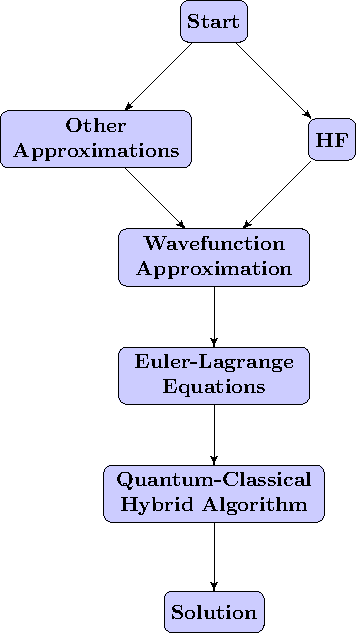
\includegraphics[width=.7\linewidth]{flowcharts/flowchart1.pdf}
  \caption{Abbreviated flowchart of the process to obtain a more accurate wavefunction for our electrons}
  \label{fig:flowchart1}
\end{figure}

\section{\textbf{\gls{tdvp}}}\label{sec:tdvp}
%\shortcite{broeckhove} \cite{kramer}
First, we must obtain an approximation of the wavefunction for our simulation. That is done by applying a unitary transformation $\hat U$ to a initial state $\ket 0$.
We find the \gls {hf} approximation by following through Fukutome's method\cite{fukutome}. After doing so, we need to derive the dynamics of our system.

\subsection{\textbf{Wavefunction approximation}}

Here we obtain an expression for our wavefunction using the \gls{hf} method: $\ket\Psi = \bm u_\lambda \ket 0$.
One approximation we can introduce here is that $\uparrow$ spin orbitals only mix with $\uparrow$ spin orbitals, and
$\downarrow$ spin orbitals only mix with $\downarrow$ spin orbitals.
Applying this to decompose $\bm u_\lambda$:
\begin{equation}
	\begin{split}
	\label {eq:udecomposition}
	u_\lambda
	= \bigotimes_{\uo 0 \oo 0} u_{\lambda_{\uo 0 \oo 0}}
	\end{split}
\end{equation}

Where we have:

\begin{align*}
	\bm u_{\lambda_{\uo 0 \oo 0}} 
	&= \begin{bmatrix}\bm C(\lambda_{\uo 0 \oo 0}) & \bm -\bm S^\dagger(\lambda_{\uo 0 \oo 0}) \\ \bm S(\lambda_{\uo 0 \oo 0}) & \tilde {\bm C}(\lambda_{\uo 0 \oo 0})\end{bmatrix} \in \mathbb{\bm C}^{2\times 2}
\end{align*}

 Since 
$\bm u_{\lambda_\ind 0} \in \mathbb{C}^{2\times2}$, it is a single-qubit operator, and each of 
$\bm C(\lambda)$, $\bm S(\lambda)$, $\tilde {\bm C}(\lambda)$
have to be a complex number, as is $\lambda$. After some calculation, their values are:
\begin{align*}
	S(\lambda_\ind 0) 
	&= \sum_{k=0}^\infty \frac{(-1)^k}{(2k + 1)!}\lambda_\ind 0({\lambda_\ind 0}^\dagger{\lambda_\ind 0})^k \\
	&= \sum_{k=0}^\infty \frac{(-1)^k}{(2k + 1)!}\lambda_\ind 0({\lambda_\ind 0}^*\lambda_\ind 0)^k \\
	&= \sum_{k=0}^\infty \frac{(-1)^k}{(2k + 1)!}\lambda_\ind 0\frac{\abs{\lambda_\ind 0}}{\abs{\lambda_\ind 0}}(\abs{\lambda_\ind 0}^2)^k \\
	&= \sum_{k=0}^\infty \frac{(-1)^k}{(2k + 1)!}\frac{\lambda_\ind 0}{\paren{\lambda_\ind 0{\lambda_\ind 0}^*}^\frac 1 2}\abs{\lambda_\ind 0}^{2k + 1} \\
	&= \sum_{k=0}^\infty \frac{(-1)^k}{(2k + 1)!}\paren{\frac{\lambda_\ind 0}{\lambda_\ind 0^*}}^\frac 1 2\abs{\lambda_\ind 0}^{2k + 1} \\
	&= \paren{\frac{\lambda_\ind 0}{\lambda_\ind 0^*}}^\frac 1 2\sum_{k=0}^\infty \frac{(-1)^k}{(2k + 1)!}\abs{\lambda_\ind 0}^{2k + 1} \\
	&= \paren{\frac{\lambda_\ind 0}{\lambda_\ind 0^*}}^\frac 1 2\s{\abs{\lambda_\ind 0}} 
\end{align*}
\begin{align*}
	S^\dagger({\lambda_\ind 0}) 
	&= \paren{\paren{\frac{\lambda_\ind 0}{\lambda_\ind 0^*}}^\frac 1 2\s{\abs{\lambda_\ind 0}}}^\dagger \\
	&= \paren{\paren{\frac{\lambda_\ind 0}{\lambda_\ind 0^*}}^\frac 1 2\s{\abs{\lambda_\ind 0}}}^* \\
	&= \paren{\frac{\lambda_\ind 0^*}{\lambda_\ind 0}}^\frac 1 2\s{\abs{\lambda_\ind 0}} 
\end{align*}
\begin{align*}
	C(\lambda_\ind 0) 
	&= I_n + \sum_{k=1}^\infty \frac{(-1)^k}{(2k)!}(\lambda_\ind 0^\dagger{\lambda_\ind 0})^k \\
	&= 1 + \sum_{k=1}^\infty \frac{(-1)^k}{(2k)!}(\lambda_\ind 0^*{\lambda_\ind 0})^k \\
	&= \sum_{k=0}^\infty \frac{(-1)^k}{(2k)!}(\abs{\lambda_\ind 0}^2)^k \\
	&= \sum_{k=0}^\infty \frac{(-1)^k}{(2k)!}\abs{\lambda_\ind 0}^{2k} \\
	&= \co {\abs{\lambda_\ind 0}} 
\end{align*}
\begin{align*}
	\tilde C({\lambda_\ind 0}) 
	&= I_{(N-n)} + \sum_{k=1}^\infty \frac{(-1)^k}{(2k)!}(\lambda_\ind 0{\lambda_\ind 0}^\dagger)^k \\
	&= 1 + \sum_{k=1}^\infty \frac{(-1)^k}{(2k)!}(\lambda_\ind 0{\lambda_\ind 0}^*)^k \\
	&= \sum_{k=0}^\infty \frac{(-1)^k}{(2k)!}\abs{\lambda_\ind 0}^{2k} \\
	&= \co {\abs{\lambda_\ind 0}} 
\end{align*}

Theorem 4.1 from \cite{nielsen} that states that a single qubit unitary gate $U$ can be written as $U = \exp(i\alpha) R_z(\beta)R_y(\gamma)R_z(\delta)$ in terms of 4 real variables $\alpha, \beta, \gamma, \delta$.
We can now apply the theorem to decompose this unitary matrix:

\begin{align*}
	\bm u_{\lambda_\ind 0}
	&= \begin{bmatrix}
		\co{\abs{\lambda_\ind 0}} & -\left(\frac{{\lambda_\ind 0}^*}{\lambda_\ind 0}\right)^{\frac 1 2}\s{\abs{\lambda_\ind 0}} \\
		\left(\frac{{\lambda_\ind 0}}{{\lambda_\ind 0}^*}\right)^{\frac 1 2}\s{\abs{\lambda_\ind 0}} &  \co{\abs{\lambda_\ind 0}}
	\end{bmatrix}\\
	&= e^{i\alpha}R_z(\beta)R_y(\gamma)R_z(\delta) 
\end{align*}

\begin{align*}
	\bm u_{\lambda_\ind 0}
	&= \begin{bmatrix}
		C(\lambda_\ind 0) & \textbf -S^\dagger({\lambda_\ind 0}) \\ 
		S(\lambda_\ind 0) & \tilde C({\lambda_\ind 0})
	\end{bmatrix} \\
	&= \begin{bmatrix}
		\co{\abs{\lambda_\ind 0}} & -\left(\frac{\lambda_\ind 0^*}{\lambda_\ind 0}\right)^{\frac 1 2}\s{\abs{\lambda_\ind 0}} \\
		\left(\frac{\lambda_\ind 0}{\lambda_\ind 0^*}\right)^{\frac 1 2}\s{\abs{\lambda_\ind 0}} &  \co{\abs{\lambda_\ind 0}}
	\end{bmatrix}\\
	&= \begin{bmatrix}
		\co{\rho_\ind 0} & -e^{-i\omega_\ind 0}\s{\rho_\ind 0} \\
		e^{i\omega_\ind 0}\s{\rho_\ind 0} &  \co{\rho_\ind 0}
	\end{bmatrix}\\
	&= \begin{bmatrix}
		e^{i\left(\alpha - \frac \beta 2 + \frac \delta 2 \right)}\co{\frac \gamma 2} & -e^{i\left(\alpha - \frac \beta 2 + \frac \delta 2 \right)}\s{\frac \gamma 2} \\
		e^{i\left(\alpha - \frac \beta 2 + \frac \delta 2 \right)}\s{\frac \gamma 2} &  e^{i\left(\alpha - \frac \beta 2 + \frac \delta 2 \right)}\co{\frac \gamma 2}
	\end{bmatrix}\\
	&= e^{i\alpha}R_z(\beta)R_y(\gamma)R_z(\delta) 
\end{align*}

Solving for $\alpha, \beta, \gamma, \delta$ in terms of $\rho_\ind 0 = \abs{\lambda_\ind 0}, \omega_\ind 0 = \arg \lambda_\ind 0$, we get 
${\alpha = 0}$; 
${\beta = \omega_\ind 0}$; 
${\gamma = 2\rho_\ind 0}$;
${\delta = -\omega_\ind 0}$. Finally:
\begin{equation}
	\begin{split}
	\label{eq:urotation}
	\bm u_{\lambda_\ind 0}
	&= R_z(\omega_\ind 0)R_y(2\rho_\ind 0)R_z(-\omega_\ind 0) \\
	&= \begin{bmatrix}
		e^{-i\frac {\omega_\ind 0} 2} & 0 \\
		0 &  e^{i\frac {\omega_\ind 0} 2}
	\end{bmatrix}
	\begin{bmatrix}
		\co{\rho_\ind 0} & -\s{\rho_\ind 0} \\
		\s{\rho_\ind 0} &  \co{\rho_\ind 0}
	\end{bmatrix}
	\begin{bmatrix}
		e^{i\frac {\omega_\ind 0} 2} & 0 \\
		0 &  e^{-i\frac {\omega_\ind 0} 2}
	\end{bmatrix} 
	\end{split}
\end{equation}

Notice now $\det \bm u_{\lambda_\ind 0} = 1$, and $\bm u_{\lambda_\ind 0} \in SU(2)$.

We shall now rewrite $\bm u_{\lambda_\ind 0}$ in terms of the pauli matrices:
\begin{align*}
	\bm u_{\lambda_\ind 0}
	&= R_z(\omega_\ind 0)R_y(2\rho_\ind 0)R_z(-\omega_\ind 0) \\
	& = \paren{\co{\frac {\omega_\ind 0} 2}I - i\s{\frac {\omega_\ind 0} 2}Z}
	\paren{\co{\rho_\ind 0}I - i\s{\rho_\ind 0}Y}
	\paren{\co{\frac {\omega_\ind 0} 2}I + i\s{\frac {\omega_\ind 0} 2}Z} \\
	& = 
	\left(
		\co{\frac {\omega_\ind 0} 2} \co {\rho_\ind 0} I 
		- i\co{\frac {\omega_\ind 0} 2} \s {\rho_\ind 0} Y 
		- i\s{\frac {\omega_\ind 0} 2} \co {\rho_\ind 0} Z
	\right. \\
	&\quad \left.
		- \s{\frac {\omega_\ind 0} 2} \s {\rho_\ind 0} ZY
	\right)
	\paren{\co{\frac {\omega_\ind 0} 2}I + i\s{\frac {\omega_\ind 0} 2}Z} \\
	\intertext{As $ZY = -iX$:}
	& = 
	\left(
		\co{\frac {\omega_\ind 0} 2} \co {\rho_\ind 0} I 
		- i\co{\frac {\omega_\ind 0} 2} \s {\rho_\ind 0} Y 
		- i\s{\frac {\omega_\ind 0} 2} \co {\rho_\ind 0} Z
	\right. \\
	&\quad \left.
		+ i\s{\frac {\omega_\ind 0} 2} \s {\rho_\ind 0} X
	\right)
	\paren{\co{\frac {\omega_\ind 0} 2}I + i\s{\frac {\omega_\ind 0} 2}Z} \\
	& = 
		\cosq{\frac {\omega_\ind 0} 2} \co {\rho_\ind 0} I 
		- i\cosq{\frac {\omega_\ind 0} 2} \s {\rho_\ind 0} Y 
		- i\s{\frac {\omega_\ind 0} 2} \co{\frac {\omega_\ind 0} 2} \co {\rho_\ind 0} Z 
	\\
	& \quad 
		+ i\s{\frac {\omega_\ind 0} 2} \co{\frac {\omega_\ind 0} 2} \s {\rho_\ind 0} X 
		+ i \s{\frac {\omega_\ind 0} 2} \co{\frac {\omega_\ind 0} 2} \co {\rho_\ind 0} Z
	\\
	& \quad 
		+ \s{\frac {\omega_\ind 0} 2} \co{\frac {\omega_\ind 0} 2} \s {\rho_\ind 0} YZ
		+ \ssq{\frac {\omega_\ind 0} 2} \co {\rho_\ind 0} I
		- \ssq{\frac {\omega_\ind 0} 2} \s {\rho_\ind 0} XZ
	\intertext{Grouping up similar terms and substituting $YZ = iX$:}
	& = 
		\co {\rho_\ind 0} \paren{
		\cosq{\frac {\omega_\ind 0} 2}  I 
		+ \ssq{\frac {\omega_\ind 0} 2} I
		}
	\\
	& \quad
		+ \co {\rho_\ind 0} \paren{
		- i\s{\frac {\omega_\ind 0} 2} \co{\frac {\omega_\ind 0} 2}  Z 
		+ i \s{\frac {\omega_\ind 0} 2} \co{\frac {\omega_\ind 0} 2}  Z
		}
	\\
	& \quad 
		+ \s {\rho_\ind 0} \paren{
		- \ssq{\frac {\omega_\ind 0} 2} XZ
		- i\cosq{\frac {\omega_\ind 0} 2} Y 
		}
	\\
	& \quad 
		+ \s {\rho_\ind 0} \paren{
		i\s{\frac {\omega_\ind 0} 2} \co{\frac {\omega_\ind 0} 2} X 
		+ i\s{\frac {\omega_\ind 0} 2} \co{\frac {\omega_\ind 0} 2} X
	}
	\\
	\intertext{Simplifying some expressions and substituting $XZ = -iY$:}
	& = 
		\co {\rho_\ind 0} I
		+ \co {\rho_\ind 0} \paren{0}
		- i \s {\rho_\ind 0} \paren{
		\cosq{\frac {\omega_\ind 0} 2} Y 
		-  \ssq{\frac {\omega_\ind 0} 2} Y
		}
	\\
	& \quad 
		+ i \s \rho_\ind 0
		2\s{\frac {\omega_\ind 0} 2} \co{\frac {\omega_\ind 0} 2} X 
	\\
	& = 
		\co {\rho_\ind 0} I
		- i \s {\rho_\ind 0} \co{\omega_\ind 0} Y 
		+ i \s {\rho_\ind 0} \s{\omega_\ind 0} X
\end{align*}

For simplicity's sake, we will consider a system with two electrons and 2 virtual orbitals. That is, $\elec=2$ and $\orb=4$. 
Now, applying $\bm u_\lambda$ to a vacuum, we get:
\begin{equation}
	\begin{split}
		\label{eq:psirw}
	\ket \Psi 
	&= \bm u_{\lambda_\ind 0} \bm u_{\lambda_\ind 1} \ket 0 \\
	&= \bm u_{\lambda_\ind 0} \bm u_{\lambda_\ind 1} \ket {\psi_{\oo 0} \psi_{\oo 1} } \\
	&= \ket {\co {\rho_\ind 0} \psi_{\oo 0} + e^{i\omega_\ind 0}\s {\rho_\ind 0} \psi_{\uo 0}} \otimes
	\ket {\co {\rho_\ind 1} \psi_{\oo 1} + e^{i\omega_\ind 1}\s {\rho_\ind 1} \psi_{\uo 1}} \\
	&= \co {\rho_\ind 0 }\co {\rho_\ind 1}\ket {\psi_{\oo 0}\psi_{\oo 1}}
	+ e^{i\omega_\ind 1}\co {\rho_\ind 0 }\s {\rho_\ind 1}\ket {\psi_{\oo 0}\psi_{\uo 1}} \\
	&\quad + e^{i\omega_\ind 0 }\s {\rho_\ind 0 }\co {\rho_\ind 1}\ket{\psi_{\uo 0} \psi_{\oo 1}} 
	+ e^{i\omega_\ind 0 }e^{i\omega_\ind 1}\s {\rho_\ind 0 }\s {\rho_\ind 1}\ket{\psi_{\uo 0} \psi_{\uo 1}} 
	\end{split}
\end{equation}
Where $\bm u_{\lambda_{\ind 0}}$ acts on $\uparrow$ spin orbitals and $\bm u_{\lambda_{\ind 1}}$ acts on $\downarrow$ spin orbitals

%-------------------------------------------------------------------------------------

\section {\textbf{Dynamics}}

The next step to use the \gls{tdvp} would be to evaluate $\bm M$ and $\bm V$. To do so, we need to set up the Lagrangian and solve the Euler-Lagrange equation system.
As seen in \cite{benjamin}, we can obtain the Lagrangian of our sistem as:
\[
	L = \frac{\sandwich{\Psi(t)}{\frac{i}{2}\left(\overrightarrow{\pd t} - \overleftarrow{\pd t}\right) - \hat H}{\Psi(t)}}{\braket{\Psi(t)}{\Psi(t)}}
\]

We start by taking the derivatives of $\ket \Psi$ with respect to $\rho_\ind 0 ,\omega_\ind 0$ and $\rho_\ind 1 , \omega_\ind 1$.
\begin{align*}
	\ket \Psi 
	&= \co {\rho_\ind 0}\co {\rho_\ind 1}\ket {\psi_{\oo 0}\psi_{\oo 1}}
	+ e^{i\omega_\ind 1}\co {\rho_\ind 0 }\s {\rho_\ind 1}\ket {\psi_{\oo 0}\psi_{\uo 1}} \\
	&\quad + e^{i\omega_\ind 0}\s {\rho_\ind 0}\co {\rho_\ind 1}\ket{\psi_{\uo 0} \psi_{\oo 1}} 
	+ e^{i\omega_\ind 0}e^{i\omega_\ind 1}\s {\rho_\ind 0}\s {\rho_\ind 1}\ket{\psi_{\uo 0} \psi_{\uo 1}} 
\end{align*}
\begin{align*}
	\pd {\rho_\ind 0 } \ket \Psi 
	&= -\s {\rho_\ind 0}\co {\rho_\ind 1}\ket {\psi_{\oo 0}\psi_{\oo 1}}
	- e^{i\omega_\ind 1}\s {\rho_\ind 0 }\s {\rho_\ind 1}\ket {\psi_{\oo 0}\psi_{\uo 1}} \\
	&\quad + e^{i\omega_\ind 0}\co {\rho_\ind 0}\co {\rho_\ind 1}\ket{\psi_{\uo 0} \psi_{\oo 1}} 
	+ e^{i\omega_\ind 0}e^{i\omega_\ind 1}\co {\rho_\ind 0}\s {\rho_\ind 1}\ket{\psi_{\uo 0} \psi_{\uo 1}} 
	\\
	\pd {\omega_\ind 0} \ket \Psi 
	&= \co {\rho_\ind 0}\co {\rho_\ind 1}\ket {\psi_{\oo 0}\psi_{\oo 1}}
	+ e^{i\omega_\ind 1}\co {\rho_\ind 0 }\s {\rho_\ind 1}\ket {\psi_{\oo 0}\psi_{\uo 1}} \\
	&\quad + ie^{i\omega_\ind 0}\s {\rho_\ind 0}\co {\rho_\ind 1}\ket{\psi_{\uo 0} \psi_{\oo 1}} 
	+ ie^{i\omega_\ind 0}e^{i\omega_\ind 1}\s {\rho_\ind 0}\s {\rho_\ind 1}\ket{\psi_{\uo 0} \psi_{\uo 1}} 
	\\
	\pd {\rho_\ind 1 } \ket \Psi 
	&= -\co {\rho_\ind 0}\s {\rho_\ind 1}\ket {\psi_{\oo 0}\psi_{\oo 1}}
	+ e^{i\omega_\ind 1}\co {\rho_\ind 0 }\co {\rho_\ind 1}\ket {\psi_{\oo 0}\psi_{\uo 1}} \\
	&\quad - e^{i\omega_\ind 0}\s {\rho_\ind 0}\s {\rho_\ind 1}\ket{\psi_{\uo 0} \psi_{\oo 1}} 
	+ e^{i\omega_\ind 0}e^{i\omega_\ind 1}\s {\rho_\ind 0}\co {\rho_\ind 1}\ket{\psi_{\uo 0} \psi_{\uo 1}} 
	\\
	\pd {\omega_\ind 1} \ket \Psi 
	&= \co {\rho_\ind 0}\co {\rho_\ind 1}\ket {\psi_{\oo 0}\psi_{\oo 1}}
	+ ie^{i\omega_\ind 1}\co {\rho_\ind 0 }\s {\rho_\ind 1}\ket {\psi_{\oo 0}\psi_{\uo 1}} \\
	&\quad + e^{i\omega_\ind 0}\s {\rho_\ind 0}\co {\rho_\ind 1}\ket{\psi_{\uo 0} \psi_{\oo 1}} 
	+ ie^{i\omega_\ind 0}e^{i\omega_\ind 1}\s {\rho_\ind 0}\s {\rho_\ind 1}\ket{\psi_{\uo 0} \psi_{\uo 1}} 
\end{align*}

We can now start developing the Lagrangian:
\[
	L = \frac{\sandwich{\Psi}{\frac{i}{2}\left(\overrightarrow{\pd t} - \overleftarrow{\pd t}\right) - \hat H}{\Psi}}{\braket{\Psi}{\Psi}}
\]
	Since $\Psi$ is normalized, $\braket{\Psi}{\Psi} = 1$. Then:
\begin{equation}
\begin{split}
	\label{eq:lagrangian}
	L &= \frac{i}{2}\bra{\Psi}{\kpp t} - \frac{i}{2}{\bpp{t}}\ket{\Psi} - \sandwich{\Psi}{\hat H}{\Psi} \\
	&=	\frac{i}{2}\bra{\Psi}\paren{\kpp {\rho_\ind 0 }\dot \rho_\ind 0  
	+	\kpp {\omega_\ind 0}\dot \omega_\ind 0 
	+	\kpp {\rho_\ind 1 }\dot \rho_\ind 1  
	+	\kpp {\omega_\ind 1}\dot \omega_\ind 1} \\
	& \quad 
	- 	\paren{\bpp{\rho_\ind 0 }\dot \rho_\ind 0 
	+ 	\bpp{\omega_\ind 0}\dot \omega_\ind 0
	+ 	\bpp{\rho_\ind 1 }\dot \rho_\ind 1 
	+ 	\bpp{\omega_\ind 1}\dot \omega_\ind 1}\frac{i}{2}\ket{\Psi}
	- \sandwich{\Psi}{\hat H}{\Psi}
\end{split}
\end{equation}
Afterwards, since the Euler-Lagrange equation gives us 
\begin{align}
	\label{eq:euler-lagrange}
	\pd{x} L = \ddt \pd{\dot x} L
\end{align}
we need to take several derivatives of $L$ obtained in \ref{eq:lagrangian} in terms of 
$\omega_\ind 0, \rho_\ind 0,
\omega_\ind 1, \rho_\ind 1$.
Taking derivatives of \ref{eq:lagrangian} with regard to ${\omega_\ind 0}$:
\begin{align*}
	\pd {\omega_\ind 0}L &=
		\frac{i}{2}\bpp {\omega_\ind 0}\paren{
		\kpp {\rho_\ind 0 }\dot \rho_\ind 0  
	+	\kpp {\omega_\ind 0} \dot \omega_\ind 0 
	+	\kpp {\rho_\ind 1 } \dot \rho_\ind 1  
	+	\kpp {\omega_\ind 1} \dot \omega_\ind 1} \\
	& \quad 
	+	\frac{i}{2}\bra{\Psi}\paren{
		\kppd {\omega_\ind 0} {\rho_\ind 0 }   	\dot \rho_\ind 0  
	+	\kppn {\omega_\ind 0} {2}  			\dot \omega_\ind 0 
	+	\kppd {\omega_\ind 0} {\rho_\ind 1 }   	\dot \rho_\ind 1  
	+	\kppd {\omega_\ind 0} {\omega_\ind 1} 	\dot \omega_\ind 1} \\
	& \quad 
	- 	\paren{
		\bppd{\omega_\ind 0} {\rho_\ind 0 }	\dot \rho_\ind 0 
	+ 	\bppn{\omega_\ind 0} {2}			\dot \omega_\ind 0
	+ 	\bppd{\omega_\ind 0} {\rho_\ind 1 }	\dot \rho_\ind 1 
	+ 	\bppd{\omega_\ind 0} {\omega_\ind 1}	\dot \omega_\ind 1
	}\frac{i}{2}\ket{\Psi} \\
	& \quad 
	- 	\paren{
		\bpp{\rho_\ind 0 }\dot \rho_\ind 0 
	+ 	\bpp{\omega_\ind 0}\dot \omega_\ind 0
	+ 	\bpp{\rho_\ind 1 }\dot \rho_\ind 1 
	+ 	\bpp{\omega_\ind 1}\dot \omega_\ind 1
	}\frac{i}{2}\kpp{\omega_\ind 0} \\
	&\quad - \pd{\omega_\ind 0}\sandwich{\Psi}{\hat H}{\Psi} 
\end{align*}
And with regards to ${\dot \omega_\ind 0}$:
\begin{align*}
	\pd {\dot \omega_\ind 0}L &= 
	  \frac{i}{2}{\bra\Psi}{\kpp{\omega_\ind 0}}
	- \frac{i}{2}{\bpp{\omega_\ind 0}}{\ket\Psi}
\end{align*}
We now take the derivative of the expression above with regards to time:
\begin{align*}
	\ddt \pd {\dot \omega_\ind 0}L &= 
	\frac{i}{2}\paren{
	\bpp{\rho_\ind 0 } \kpp{\omega_\ind 0} \dot \rho_\ind 0  
	+ \bpp{\omega_\ind 0} \kpp{\omega_\ind 0} \dot \omega_\ind 0 
	+ \bpp{\rho_\ind 1 } \kpp{\omega_\ind 0} \dot \rho_\ind 1  
	+ \bpp{\omega_\ind 1} \kpp{\omega_\ind 0} \dot \omega_\ind 1 
} \\
&\quad + \frac{i}{2} \bra\Psi \paren{
		\kppd{\rho_\ind 0 }{\omega_\ind 0} \dot \rho_\ind 0 
	+	\kppd{\omega_\ind 0}{\omega_\ind 0} \dot \omega_\ind 0
	+	\kppd{\rho_\ind 1 }{\omega_\ind 0} \dot \rho_\ind 1 
	+	\kppd{\omega_\ind 1}{\omega_\ind 0} \dot \omega_\ind 1
} \\
&\quad - \frac{i}{2} \paren{
		\bppd{\rho_\ind 0 }{\omega_\ind 0} \dot \rho_\ind 0 
	+	\bppd{\omega_\ind 0}{\omega_\ind 0} \dot \omega_\ind 0
	+	\bppd{\rho_\ind 1 }{\omega_\ind 0} \dot \rho_\ind 1 
	+	\bppd{\omega_\ind 1}{\omega_\ind 0} \dot \omega_\ind 1
} \ket\Psi \\
&\quad - \frac{i}{2} \paren{
	\bpp{\omega_\ind 0} \kpp{\rho_\ind 0 } \dot \rho_\ind 0  
	+ \bpp{\omega_\ind 0} \kpp{\omega_\ind 0} \dot \omega_\ind 0 
	+ \bpp{\omega_\ind 0} \kpp{\rho_\ind 1 } \dot \rho_\ind 1  
	+ \bpp{\omega_\ind 0} \kpp{\omega_\ind 1} \dot \omega_\ind 1 
} 
\end{align*}
Now, since the Euler-Lagrange equation gives us $\pd{\omega_\ind 0} L = \ddt \pd{\dot \omega_\ind 0} L$, we can substitute the expressions obtained above and simplify our equation:
\begin{align*}
	\pd{\omega_\ind 0} L &= \ddt \pd{\dot \omega_\ind 0} L
	\\ 
		i\bpp {\omega_\ind 0}\paren{
		\kpp {\rho_\ind 0 }\dot \rho_\ind 0  
	+	\kpp {\rho_\ind 1 } \dot \rho_\ind 1  
	+	\kpp {\omega_\ind 1} \dot \omega_\ind 1} 
	&\\
	%---------------------------------------------------------------
	- 	i\paren{
		\bpp{\rho_\ind 0 }\dot \rho_\ind 0 
	+ 	\bpp{\rho_\ind 1 }\dot \rho_\ind 1 
	+ 	\bpp{\omega_\ind 1}\dot \omega_\ind 1
	}\kpp{\omega_\ind 0}
	%---------------------------------------------------------------
	&= \pd{\omega_\ind 0}\sandwich{\Psi}{\hat H}{\Psi} 
\end{align*}
Moving on to the next variable, we'll be taking derivatives of \ref{eq:lagrangian} with regard to ${\rho_\ind 0}$:
\begin{align*}
	\pd {\rho_\ind 0 }L &=
		\frac{i}{2}\bpp {\rho_\ind 0 }\paren{
		\kpp {\rho_\ind 0 }\dot \rho_\ind 0  
	+	\kpp {\omega_\ind 0} \dot \omega_\ind 0 
	+	\kpp {\rho_\ind 1 } \dot \rho_\ind 1  
	+	\kpp {\omega_\ind 1} \dot \omega_\ind 1} \\
	& \quad 
	+	\frac{i}{2}\bra{\Psi}\paren{
		\kppn {\rho_\ind 0 } {2}  			\dot \rho_\ind 0  
	+	\kppd {\rho_\ind 0 } {\omega_\ind 0}   	\dot \omega_\ind 0 
	+	\kppd {\rho_\ind 0 } {\rho_\ind 1 }   	\dot \rho_\ind 1  
	+	\kppd {\rho_\ind 0 } {\omega_\ind 1} 	\dot \omega_\ind 1} \\
	& \quad 
	- 	\paren{
	  	\bppn{\rho_\ind 0 } {2}			\dot \rho_\ind 0 
	+	\bppd{\rho_\ind 0 } {\omega_\ind 0}	\dot \omega_\ind 0
	+ 	\bppd{\rho_\ind 0 } {\rho_\ind 1 }	\dot \rho_\ind 1 
	+ 	\bppd{\rho_\ind 0 } {\omega_\ind 1}	\dot \omega_\ind 1
	}\frac{i}{2}\ket{\Psi} \\
	& \quad 
	- 	\paren{
		\bpp{\rho_\ind 0 }\dot \rho_\ind 0 
	+ 	\bpp{\omega_\ind 0}\dot \omega_\ind 0
	+ 	\bpp{\rho_\ind 1 }\dot \rho_\ind 1 
	+ 	\bpp{\omega_\ind 1}\dot \omega_\ind 1
	}\frac{i}{2}\kpp{\rho_\ind 0 } \\
	&\quad - \pd{\rho_\ind 0 }\sandwich{\Psi}{\hat H}{\Psi} 
\end{align*}
And with regards to ${\dot \rho_\ind 0}$:
\begin{align*}
	\pd {\dot \rho_\ind 0 }L &= 
	  \frac{i}{2}{\bra\Psi}{\kpp{\rho_\ind 0 }}
	- \frac{i}{2}{\bpp{\rho_\ind 0 }}{\ket\Psi}
\end{align*}
We now take the derivative of the expression above with regards to time:
\begin{align*}
	\ddt \pd {\dot \rho_\ind 0 }L &= 
	\frac{i}{2}\paren{
	\bpp{\rho_\ind 0 } \kpp{\rho_\ind 0 } \dot \rho_\ind 0  
	+ \bpp{\omega_\ind 0} \kpp{\rho_\ind 0 } \dot \omega_\ind 0 
	+ \bpp{\rho_\ind 1 } \kpp{\rho_\ind 0 } \dot \rho_\ind 1  
	+ \bpp{\omega_\ind 1} \kpp{\rho_\ind 0 } \dot \omega_\ind 1 
} \\
&\quad + \frac{i}{2} \bra\Psi \paren{
		\kppd{\rho_\ind 0 }{\rho_\ind 0 } \dot \rho_\ind 0 
	+	\kppd{\omega_\ind 0}{\rho_\ind 0 } \dot \omega_\ind 0
	+	\kppd{\rho_\ind 1 }{\rho_\ind 0 } \dot \rho_\ind 1 
	+	\kppd{\omega_\ind 1}{\rho_\ind 0 } \dot \omega_\ind 1
} \\
&\quad - \frac{i}{2} \paren{
		\bppd{\rho_\ind 0 }{\rho_\ind 0 } \dot \rho_\ind 0 
	+	\bppd{\omega_\ind 0}{\rho_\ind 0 } \dot \omega_\ind 0
	+	\bppd{\rho_\ind 1 }{\rho_\ind 0 } \dot \rho_\ind 1 
	+	\bppd{\omega_\ind 1}{\rho_\ind 0 } \dot \omega_\ind 1
} \ket\Psi \\
&\quad - \frac{i}{2} \paren{
	\bpp{\rho_\ind 0 } \kpp{\rho_\ind 0 } \dot \rho_\ind 0  
	+ \bpp{\rho_\ind 0 } \kpp{\omega_\ind 0} \dot \omega_\ind 0 
	+ \bpp{\rho_\ind 0 } \kpp{\rho_\ind 1 } \dot \rho_\ind 1  
	+ \bpp{\rho_\ind 0 } \kpp{\omega_\ind 1} \dot \omega_\ind 1 
} 
\end{align*}
Now, since the Euler-Lagrange equation gives us $\pd{\rho_\ind 0 } L = \ddt \pd{\dot \rho_\ind 0 } L$, we can substitute the expressions obtained above and simplify our equation:
\begin{align*}
	\pd{\rho_\ind 0 } L &= \ddt \pd{\dot \rho_\ind 0 } L
	\\ 
		i\bpp {\rho_\ind 0 }\paren{
		\kpp {\omega_\ind 0}\dot \omega_\ind 0
	+	\kpp {\rho_\ind 1 } \dot \rho_\ind 1  
	+	\kpp {\omega_\ind 1} \dot \omega_\ind 1} 
	&\\
	%---------------------------------------------------------------
	- 	i\paren{
		\bpp{\omega_\ind 0}\dot \omega_\ind 0
	+ 	\bpp{\rho_\ind 1 }\dot \rho_\ind 1 
	+ 	\bpp{\omega_\ind 1}\dot \omega_\ind 1
	}\kpp{\rho_\ind 0 }
	%---------------------------------------------------------------
	&= \pd{\rho_\ind 0 }\sandwich{\Psi}{\hat H}{\Psi}
\end{align*}
For the next variable, we'll be taking derivatives of \ref{eq:lagrangian} with regard to ${\omega_\ind 1}$:
\begin{align*}
	\pd {\omega_\ind 1}L &=
		\frac{i}{2}\bpp {\omega_\ind 1}\paren{
		\kpp {\rho_\ind 0 }\dot \rho_\ind 0  
	+	\kpp {\omega_\ind 0} \dot \omega_\ind 0 
	+	\kpp {\rho_\ind 1 } \dot \rho_\ind 1  
	+	\kpp {\omega_\ind 1} \dot \omega_\ind 1} \\
	& \quad 
	+	\frac{i}{2}\bra{\Psi}\paren{
		\kppd {\omega_\ind 1} {\rho_\ind 0 }   	\dot \rho_\ind 0  
	+	\kppd {\omega_\ind 1} {\omega_\ind 0}	\dot \omega_\ind 0 
	+	\kppd {\omega_\ind 1} {\rho_\ind 1 }   	\dot \rho_\ind 1  
	+	\kppn {\omega_\ind 1} 2		 	\dot \omega_\ind 1} \\
	& \quad 
	- 	\paren{
		\bppd{\omega_\ind 1} {\rho_\ind 0 }	\dot \rho_\ind 0 
	+ 	\bppd{\omega_\ind 1} {\omega_\ind 0}	\dot \omega_\ind 0
	+ 	\bppd{\omega_\ind 1} {\rho_\ind 1 }	\dot \rho_\ind 1 
	+ 	\bppn{\omega_\ind 1} 2			\dot \omega_\ind 1
	}\frac{i}{2}\ket{\Psi} \\
	& \quad 
	- 	\paren{
		\bpp{\rho_\ind 0 }\dot \rho_\ind 0 
	+ 	\bpp{\omega_\ind 0}\dot \omega_\ind 0
	+ 	\bpp{\rho_\ind 1 }\dot \rho_\ind 1 
	+ 	\bpp{\omega_\ind 1}\dot \omega_\ind 1
	}\frac{i}{2}\kpp{\omega_\ind 1} \\
	&\quad - \pd{\omega_\ind 1}\sandwich{\Psi}{\hat H}{\Psi}
\end{align*}
And with regards to ${\dot \omega_\ind 1}$:
\begin{align*}
	\pd {\dot \omega_\ind 1}L &= 
	  \frac{i}{2}{\bra\Psi}{\kpp{\omega_\ind 1}}
	- \frac{i}{2}{\bpp{\omega_\ind 1}}{\ket\Psi}
\end{align*}
We now take the derivative of the expression above with regards to time:
\begin{align*}
	\ddt \pd {\dot \omega_\ind 1}L &= 
	\frac{i}{2}\paren{
	\bpp{\rho_\ind 0 } \kpp{\omega_\ind 1} \dot \rho_\ind 0  
	+ \bpp{\omega_\ind 0} \kpp{\omega_\ind 1} \dot \omega_\ind 0 
	+ \bpp{\rho_\ind 1 } \kpp{\omega_\ind 1} \dot \rho_\ind 1  
	+ \bpp{\omega_\ind 1} \kpp{\omega_\ind 1} \dot \omega_\ind 1 
} \\
&\quad + \frac{i}{2} \bra\Psi \paren{
		\kppd{\rho_\ind 0 }{\omega_\ind 1} \dot \rho_\ind 0 
	+	\kppd{\omega_\ind 0}{\omega_\ind 1} \dot \omega_\ind 0
	+	\kppd{\rho_\ind 1 }{\omega_\ind 1} \dot \rho_\ind 1 
	+	\kppd{\omega_\ind 1}{\omega_\ind 1} \dot \omega_\ind 1
} \\
&\quad - \frac{i}{2} \paren{
		\bppd{\rho_\ind 0 }{\omega_\ind 1} \dot \rho_\ind 0 
	+	\bppd{\omega_\ind 0}{\omega_\ind 1} \dot \omega_\ind 0
	+	\bppd{\rho_\ind 1 }{\omega_\ind 1} \dot \rho_\ind 1 
	+	\bppd{\omega_\ind 1}{\omega_\ind 1} \dot \omega_\ind 1
} \ket\Psi \\
&\quad - \frac{i}{2} \paren{
	\bpp{\omega_\ind 1} \kpp{\rho_\ind 0 } \dot \rho_\ind 0  
	+ \bpp{\omega_\ind 1} \kpp{\omega_\ind 0} \dot \omega_\ind 0 
	+ \bpp{\omega_\ind 1} \kpp{\rho_\ind 1 } \dot \rho_\ind 1  
	+ \bpp{\omega_\ind 1} \kpp{\omega_\ind 1} \dot \omega_\ind 1 
}
\end{align*}
Now, since the Euler-Lagrange equation gives us $\pd{\omega_\ind 1} L = \ddt \pd{\dot \omega_\ind 1} L$, we can substitute the expressions obtained above and simplify our equation:
\begin{align*}
	\pd{\omega_\ind 1} L &= \ddt \pd{\dot \omega_\ind 1} L
	\\ 
		i\bpp {\omega_\ind 1}\paren{
		\kpp {\rho_\ind 0 }\dot \rho_\ind 0  
	+	\kpp {\omega_\ind 0} \dot \omega_\ind 0
	+	\kpp {\rho_\ind 1 } \dot \rho_\ind 1 }
	&\\
	%---------------------------------------------------------------
	- 	i\paren{
		\bpp{\rho_\ind 0 }\dot \rho_\ind 0 
	+ 	\bpp{\omega_\ind 0}\dot \omega_\ind 0
	+ 	\bpp{\rho_\ind 1 }\dot \rho_\ind 1 
	}\kpp{\omega_\ind 1}
	%---------------------------------------------------------------
	&= \pd{\omega_\ind 1}\sandwich{\Psi}{\hat H}{\Psi} 
\end{align*}
For the next variable, we'll be taking derivatives of \ref{eq:lagrangian} with regard to ${\rho_\ind 1}$:
\begin{align*}
	\pd {\rho_\ind 1 }L &=
		\frac{i}{2}\bpp {\rho_\ind 1 }\paren{
		\kpp {\rho_\ind 0 }\dot \rho_\ind 0  
	+	\kpp {\omega_\ind 0} \dot \omega_\ind 0 
	+	\kpp {\rho_\ind 1 } \dot \rho_\ind 1  
	+	\kpp {\omega_\ind 1} \dot \omega_\ind 1} \\
	& \quad 
	+	\frac{i}{2}\bra{\Psi}\paren{
		\kppd {\rho_\ind 1 } {\rho_\ind 0 }   	\dot \rho_\ind 0  
	+	\kppd {\rho_\ind 1 } {\omega_\ind 0}   	\dot \omega_\ind 0 
	+	\kppn {\rho_\ind 1 } {2}  			\dot \rho_\ind 1  
	+	\kppd {\rho_\ind 1 } {\omega_\ind 1} 	\dot \omega_\ind 1} \\
	& \quad 
	- 	\paren{
	 	\bppd{\rho_\ind 1 } {\rho_\ind 0 }	\dot \rho_\ind 0 
	+	\bppd{\rho_\ind 1 } {\omega_\ind 0}	\dot \omega_\ind 0
	+  	\bppn{\rho_\ind 1 } {2}			\dot \rho_\ind 1 
	+ 	\bppd{\rho_\ind 1 } {\omega_\ind 1}	\dot \omega_\ind 1
	}\frac{i}{2}\ket{\Psi} \\
	& \quad 
	- 	\paren{
		\bpp{\rho_\ind 0 }\dot \rho_\ind 0 
	+ 	\bpp{\omega_\ind 0}\dot \omega_\ind 0
	+ 	\bpp{\rho_\ind 1 }\dot \rho_\ind 1 
	+ 	\bpp{\omega_\ind 1}\dot \omega_\ind 1
	}\frac{i}{2}\kpp{\rho_\ind 1 } \\
	&\quad - \pd{\rho_\ind 1 }\sandwich{\Psi}{\hat H}{\Psi}
\end{align*}
And with regards to ${\dot \rho_\ind 1}$:
\begin{align*}
	\pd {\dot \rho_\ind 1 }L &= 
	  \frac{i}{2}{\bra\Psi}{\kpp{\rho_\ind 1 }}
	- \frac{i}{2}{\bpp{\rho_\ind 1 }}{\ket\Psi}
\end{align*}
We now take the derivative of the expression above with regards to time:
\begin{align*}
	\ddt \pd {\dot \rho_\ind 1 }L &= 
	\frac{i}{2}\paren{
	\bpp{\rho_\ind 0 } \kpp{\rho_\ind 1 } \dot \rho_\ind 0  
	+ \bpp{\omega_\ind 0} \kpp{\rho_\ind 1 } \dot \omega_\ind 0 
	+ \bpp{\rho_\ind 1 } \kpp{\rho_\ind 1 } \dot \rho_\ind 1  
	+ \bpp{\omega_\ind 1} \kpp{\rho_\ind 1 } \dot \omega_\ind 1 
} \\
&\quad + \frac{i}{2} \bra\Psi \paren{
		\kppd{\rho_\ind 0 }{\rho_\ind 1 } \dot \rho_\ind 0 
	+	\kppd{\omega_\ind 0}{\rho_\ind 1 } \dot \omega_\ind 0
	+	\kppd{\rho_\ind 1 }{\rho_\ind 1 } \dot \rho_\ind 1 
	+	\kppd{\omega_\ind 1}{\rho_\ind 1 } \dot \omega_\ind 1
} \\
&\quad - \frac{i}{2} \paren{
		\bppd{\rho_\ind 0 }{\rho_\ind 1 } \dot \rho_\ind 0 
	+	\bppd{\omega_\ind 0}{\rho_\ind 1 } \dot \omega_\ind 0
	+	\bppd{\rho_\ind 1 }{\rho_\ind 1 } \dot \rho_\ind 1 
	+	\bppd{\omega_\ind 1}{\rho_\ind 1 } \dot \omega_\ind 1
} \ket\Psi \\
&\quad - \frac{i}{2} \paren{
	\bpp{\rho_\ind 1 } \kpp{\rho_\ind 0 } \dot \rho_\ind 0  
	+ \bpp{\rho_\ind 1 } \kpp{\omega_\ind 0} \dot \omega_\ind 0 
	+ \bpp{\rho_\ind 1 } \kpp{\rho_\ind 1 } \dot \rho_\ind 1  
	+ \bpp{\rho_\ind 1 } \kpp{\omega_\ind 1} \dot \omega_\ind 1 
}
\end{align*}
Now, since the Euler-Lagrange equation gives us $\pd{\rho_\ind 1} L = \ddt \pd{\dot \rho_\ind 1} L$, we can substitute the expressions obtained above and simplify our equation:
\begin{align*}
	\pd{\rho_\ind 1 } L &= \ddt \pd{\dot \rho_\ind 1 } L
	\\ 
		i\bpp {\rho_\ind 1 }\paren{
		\kpp {\rho_\ind 0 } \dot \rho_\ind 0  
	+	\kpp {\omega_\ind 0}\dot \omega_\ind 0
	+	\kpp {\omega_\ind 1} \dot \omega_\ind 1} 
	&\\
	%---------------------------------------------------------------
	- 	i\paren{
	 	\bpp{\rho_\ind 0 }\dot \rho_\ind 0 
	+	\bpp{\omega_\ind 0}\dot \omega_\ind 0
	+ 	\bpp{\omega_\ind 1}\dot \omega_\ind 1
	}\kpp{\rho_\ind 1 }
	%---------------------------------------------------------------
	&= \pd{\rho_\ind 1 }\sandwich{\Psi}{\hat H}{\Psi}
\end{align*}
After all these steps, we obtain the following system of equations from \ref{eq:euler-lagrange}:
\begin{equation}
\begin{split}
	\label {eq:prematrixrw}
	- 	i\paren{
		\bpp{\omega_\ind 0}\dot \omega_\ind 0
	+ 	\bpp{\rho_\ind 1 }\dot \rho_\ind 1 
	+ 	\bpp{\omega_\ind 1}\dot \omega_\ind 1
	}\kpp{\rho_\ind 0 }
	%---------------------------------------------------------------
	&= \pd{\rho_\ind 0 }\sandwich{\Psi}{\hat H}{\Psi} \\
		i\bpp {\omega_\ind 0}\paren{
		\kpp {\rho_\ind 0 }\dot \rho_\ind 0  
	+	\kpp {\rho_\ind 1 } \dot \rho_\ind 1  
	+	\kpp {\omega_\ind 1} \dot \omega_\ind 1} 
	&\\
	%---------------------------------------------------------------
	- 	i\paren{
		\bpp{\rho_\ind 0 }\dot \rho_\ind 0 
	+ 	\bpp{\rho_\ind 1 }\dot \rho_\ind 1 
	+ 	\bpp{\omega_\ind 1}\dot \omega_\ind 1
	}\kpp{\omega_\ind 0}
	%---------------------------------------------------------------
	&= \pd{\omega_\ind 0}\sandwich{\Psi}{\hat H}{\Psi} \\
		i\bpp {\rho_\ind 1 }\paren{
		\kpp {\rho_\ind 0 } \dot \rho_\ind 0  
	+	\kpp {\omega_\ind 0}\dot \omega_\ind 0
	+	\kpp {\omega_\ind 1} \dot \omega_\ind 1} 
	&\\
	%---------------------------------------------------------------
	- 	i\paren{
	 	\bpp{\rho_\ind 0 }\dot \rho_\ind 0 
	+	\bpp{\omega_\ind 0}\dot \omega_\ind 0
	+ 	\bpp{\omega_\ind 1}\dot \omega_\ind 1
	}\kpp{\rho_\ind 1 }
	%---------------------------------------------------------------
	&= \pd{\rho_\ind 1 }\sandwich{\Psi}{\hat H}{\Psi} \\
		i\bpp {\rho_\ind 0 }\paren{
		\kpp {\omega_\ind 0}\dot \omega_\ind 0
	+	\kpp {\rho_\ind 1 } \dot \rho_\ind 1  
	+	\kpp {\omega_\ind 1} \dot \omega_\ind 1} 
	&\\
	%---------------------------------------------------------------
	- 	i\paren{
		\bpp{\rho_\ind 0 }\dot \rho_\ind 0 
	+ 	\bpp{\omega_\ind 0}\dot \omega_\ind 0
	+ 	\bpp{\rho_\ind 1 }\dot \rho_\ind 1 
	}\kpp{\omega_\ind 1}
	%---------------------------------------------------------------
	&= \pd{\omega_\ind 1}\sandwich{\Psi}{\hat H}{\Psi} \\
		i\bpp {\rho_\ind 0 }\paren{
		\kpp {\omega_\ind 0}\dot \omega_\ind 0
	+	\kpp {\rho_\ind 1 } \dot \rho_\ind 1  
	+	\kpp {\omega_\ind 1} \dot \omega_\ind 1} 
	&\\
	%---------------------------------------------------------------
\end{split}
\end{equation}
We can put the system of equations in matrix form:
\begin{equation}
\begin{split}
	\label {eq:matrixderiv}
	&\begin{bmatrix}
		&0
		& \bpp{\rho_\ind 0} \kpp{\omega_\ind 0}
		- \bpp{\omega_\ind 0} \kpp{\rho_\ind 0}
		& \bpp{\rho_\ind 0} \kpp{\rho_\ind 1}
		- \bpp{\rho_\ind 1} \kpp{\rho_\ind 0}
		& \bpp{\rho_\ind 0} \kpp{\omega_\ind 1}
		- \bpp{\omega_\ind 1} \kpp{\rho_\ind 0}
		\\
		& \bpp{\omega_\ind 0} \kpp{\rho_\ind 0}
		- \bpp{\rho_\ind 0} \kpp{\omega_\ind 0}
		&0
		& \bpp{\omega_\ind 0} \kpp{\rho_\ind 1}
		- \bpp{\rho_\ind 1} \kpp{\omega_\ind 0}
		& \bpp{\omega_\ind 0} \kpp{\omega_\ind 1}
		- \bpp{\omega_\ind 1} \kpp{\omega_\ind 0}
		\\
		& \bpp{\rho_\ind 1} \kpp{\rho_\ind 0}
		- \bpp{\rho_\ind 0} \kpp{\rho_\ind 1}
		& \bpp{\rho_\ind 1} \kpp{\omega_\ind 0}
		- \bpp{\omega_\ind 0} \kpp{\rho_\ind 1}
		&0
		& \bpp{\rho_\ind 1} \kpp{\omega_\ind 1}
		- \bpp{\omega_\ind 1} \kpp{\rho_\ind 1}
		\\
		& \bpp{\omega_\ind 1} \kpp{\rho_\ind 0}
		- \bpp{\rho_\ind 0} \kpp{\omega_\ind 1}
		& \bpp{\omega_\ind 1} \kpp{\omega_\ind 0}
		- \bpp{\omega_\ind 0} \kpp{\omega_\ind 1}
		& \bpp{\omega_\ind 1} \kpp{\rho_\ind 1}
		- \bpp{\rho_\ind 1} \kpp{\omega_\ind 1}
		&0
		\\
	\end{bmatrix}
      	\\
	&\times	i
	\begin{bmatrix}
		\dot \rho_\ind 0 \\
		\dot \omega_\ind 0 \\
		\dot \rho_\ind 1 \\
		\dot \omega_\ind 1 \\
	\end{bmatrix}
	= 
	\begin{bmatrix}
	&\pd{\rho_\ind 0}\sandwich{\Psi}{\hat H}{\Psi} \\
	&\pd{\omega_\ind 0}\sandwich{\Psi}{\hat H}{\Psi} \\
	&\pd{\rho_\ind 1}\sandwich{\Psi}{\hat H}{\Psi} \\
	&\pd{\omega_\ind 1}\sandwich{\Psi}{\hat H}{\Psi} \\
	\end{bmatrix}
\end{split}
\end{equation}
Now we need to evaluate the elements of the matrix. We already have the partial derivatives of $\ket\Psi$, but we need to find the expressions for their duals. We can take the dual of $\ket \Psi$ from \ref{eq:psirw}:
\begin{equation}
	\label{eq:dualpsirw}
	\begin{split}
		\bra \Psi &= \ket\Psi^\dagger
	= \left(\co {\rho_\ind 0 }\co {\rho_\ind 1}\ket {\psi_{\oo 0}\psi_{\oo 1}}
	+ e^{i\omega_\ind 1}\co {\rho_\ind 0 }\s {\rho_\ind 1}\ket {\psi_{\oo 0}\psi_{\uo 1}} \right .\\
	& \left . \quad + e^{i\omega_\ind 0 }\s {\rho_\ind 0 }\co {\rho_\ind 1}\ket{\psi_{\uo 0} \psi_{\oo 1}} 
	+ e^{i\omega_\ind 0 }e^{i\omega_\ind 1}\s {\rho_\ind 0 }\s {\rho_\ind 1}\ket{\psi_{\uo 0} \psi_{\uo 1}} \right)^\dagger \\
	&= \co {\rho_\ind 0}\co {\rho_\ind 1}\bra {\psi_{\oo 0}\psi_{\oo 1}}
	+ e^{ -i \omega_\ind 1}\co {\rho_\ind 0 }\s {\rho_\ind 1}\bra {\psi_{\oo 0}\psi_{\uo 1}} \\
	&\quad + e^{ -i \omega_\ind 0}\s {\rho_\ind 0}\co {\rho_\ind 1}\bra{\psi_{\uo 0} \psi_{\oo 1}} 
	+ e^{ -i \omega_\ind 0}e^{ -i \omega_\ind 1}\s {\rho_\ind 0}\s {\rho_\ind 1}\bra{\psi_{\uo 0} \psi_{\uo 1}} 
	\end{split}
\end{equation}
And take the derivatives of \ref{eq:dualpsirw}:
\begin{align*}
	\pd {\rho_\ind 0 } \bra \Psi 
	&= -\s {\rho_\ind 0}\co {\rho_\ind 1}\bra {\psi_{\oo 0}\psi_{\oo 1}}
	- e^{ -i \omega_\ind 1}\s {\rho_\ind 0 }\s {\rho_\ind 1}\bra {\psi_{\oo 0}\psi_{\uo 1}} \\
	&\quad + e^{ -i \omega_\ind 0}\co {\rho_\ind 0}\co {\rho_\ind 1}\bra{\psi_{\uo 0} \psi_{\oo 1}} 
	+ e^{ -i \omega_\ind 0}e^{ -i \omega_\ind 1}\co {\rho_\ind 0}\s {\rho_\ind 1}\bra{\psi_{\uo 0} \psi_{\uo 1}} 
	\\
	\pd {\omega_\ind 0} \bra \Psi 
	&=
	-i e^{ -i \omega_\ind 0}\s {\rho_\ind 0}\co {\rho_\ind 1}\bra{\psi_{\uo 0} \psi_{\oo 1}} 
	-i e^{ -i \omega_\ind 0}e^{ -i \omega_\ind 1}\s {\rho_\ind 0}\s {\rho_\ind 1}\bra{\psi_{\uo 0} \psi_{\uo 1}} 
	\\
	\pd {\rho_\ind 1 } \bra \Psi 
	&= -\co {\rho_\ind 0}\s {\rho_\ind 1}\bra {\psi_{\oo 0}\psi_{\oo 1}}
	+ e^{ -i \omega_\ind 1}\co {\rho_\ind 0 }\co {\rho_\ind 1}\bra {\psi_{\oo 0}\psi_{\uo 1}} \\
	&\quad - e^{ -i \omega_\ind 0}\s {\rho_\ind 0}\s {\rho_\ind 1}\bra{\psi_{\uo 0} \psi_{\oo 1}} 
	+ e^{ -i \omega_\ind 0}e^{ -i \omega_\ind 1}\s {\rho_\ind 0}\co {\rho_\ind 1}\bra{\psi_{\uo 0} \psi_{\uo 1}} 
	\\
	\pd {\omega_\ind 1} \bra \Psi 
	&= 
	-i e^{ -i \omega_\ind 1}\co {\rho_\ind 0 }\s {\rho_\ind 1}\bra {\psi_{\oo 0}\psi_{\uo 1}}
	-i e^{ -i \omega_\ind 0}e^{ -i \omega_\ind 1}\s {\rho_\ind 0}\s {\rho_\ind 1}\bra{\psi_{\uo 0} \psi_{\uo 1}} 
\end{align*}
Finally, we have all the information needed to calculate the elements of the first matrix in \ref{eq:matrixderiv}. First, we notice that the matrix is skew-symmetric, since:

\begin{align*}
	\bpp{\omega_\ind 0} \kpp{\rho_\ind 0}
	- \bpp{\rho_\ind 0} \kpp{\omega_\ind 0} = 
	- \paren
	{
		\bpp{\rho_\ind 0} \kpp{\omega_\ind 0} 
		-\bpp{\omega_\ind 0} \kpp{\rho_\ind 0}
	}
\end{align*}

\begin{enumerate}
	% item I
	\item $ \bpp{\rho_\ind 0} \kpp{\omega_\ind 0}
	- \bpp{\omega_\ind 0} \kpp{\rho_\ind 0}$

\begin{align*}
	&\left (
	-\s {\rho_\ind 0}\co {\rho_\ind 1}\bra {\psi_{\oo 0}\psi_{\oo 1}}
	- e^{ -i \omega_\ind 1}\s {\rho_\ind 0 }\s {\rho_\ind 1}\bra {\psi_{\oo 0}\psi_{\uo 1}}
	\right .
	\\
	&\left .
	\quad + e^{ -i \omega_\ind 0}\co {\rho_\ind 0}\co {\rho_\ind 1}\bra{\psi_{\uo 0} \psi_{\oo 1}} 
	+ e^{ -i \omega_\ind 0}e^{ -i \omega_\ind 1}\co {\rho_\ind 0}\s {\rho_\ind 1}\bra{\psi_{\uo 0} \psi_{\uo 1}} 
	\right )
	\\
	&\times \left (
	ie^{i\omega_\ind 0}\s {\rho_\ind 0}\co {\rho_\ind 1}\ket{\psi_{\uo 0} \psi_{\oo 1}} 
	+ ie^{i\omega_\ind 0}e^{i\omega_\ind 1}\s {\rho_\ind 0}\s {\rho_\ind 1}\ket{\psi_{\uo 0} \psi_{\uo 1}} 
	\right )
	\\
	&- \left (
	-i e^{ -i \omega_\ind 0}\s {\rho_\ind 0}\co {\rho_\ind 1}\bra{\psi_{\uo 0} \psi_{\oo 1}} 
	-i e^{ -i \omega_\ind 0}e^{ -i \omega_\ind 1}\s {\rho_\ind 0}\s {\rho_\ind 1}\bra{\psi_{\uo 0} \psi_{\uo 1}} 
	\right )
	\\
	&\times\left (
	-\s {\rho_\ind 0}\co {\rho_\ind 1}\ket {\psi_{\oo 0}\psi_{\oo 1}}
	- e^{i\omega_\ind 1}\s {\rho_\ind 0 }\s {\rho_\ind 1}\ket {\psi_{\oo 0}\psi_{\uo 1}}
	\right .
	\\
	&\left .
	\quad + e^{i\omega_\ind 0}\co {\rho_\ind 0}\co {\rho_\ind 1}\ket{\psi_{\uo 0} \psi_{\oo 1}} 
	+ e^{i\omega_\ind 0}e^{i\omega_\ind 1}\co {\rho_\ind 0}\s {\rho_\ind 1}\ket{\psi_{\uo 0} \psi_{\uo 1}} 
	\right )
	\intertext{Since we have an orthogonal basis, only matching brackets are nonzero:}
	% --------------------------------------Second System-----------------------------------
	&=
		i\s{\rho_\ind 0} \co{\rho_\ind 0}\cosq {\rho_\ind 1}
		+ i\s{\rho_\ind 0} \co{\rho_\ind 0}\ssq {\rho_\ind 1}
	\\
	&+
	i \s {\rho_\ind 0}\co {\rho_\ind 0}\cosq {\rho_\ind 1}
	+i \s {\rho_\ind 0}\co {\rho_\ind 0}\ssq {\rho_\ind 1}
	\\
	&=
	i\s{2\rho_\ind 0}
\end{align*}

	% item II
	\item $ \bpp{\rho_\ind 0} \kpp{\rho_\ind 1}
	- \bpp{\rho_\ind 1} \kpp{\rho_\ind 0}$


\begin{align*}
	&\left (
	-\s {\rho_\ind 0}\co {\rho_\ind 1}\bra {\psi_{\oo 0}\psi_{\oo 1}}
	- e^{ -i \omega_\ind 1}\s {\rho_\ind 0 }\s {\rho_\ind 1}\bra {\psi_{\oo 0}\psi_{\uo 1}} 
	\right .
	\\
	&\left .
	\quad + e^{ -i \omega_\ind 0}\co {\rho_\ind 0}\co {\rho_\ind 1}\bra{\psi_{\uo 0} \psi_{\oo 1}} 
	+ e^{ -i \omega_\ind 0}e^{ -i \omega_\ind 1}\co {\rho_\ind 0}\s {\rho_\ind 1}\bra{\psi_{\uo 0} \psi_{\uo 1}} 
	\right )
	\\
	&\times\left (
	-\co {\rho_\ind 0}\s {\rho_\ind 1}\ket {\psi_{\oo 0}\psi_{\oo 1}}
	+ e^{i\omega_\ind 1}\co {\rho_\ind 0 }\co {\rho_\ind 1}\ket {\psi_{\oo 0}\psi_{\uo 1}} 
	\right .
	\\
	&\left .
	\quad - e^{i\omega_\ind 0}\s {\rho_\ind 0}\s {\rho_\ind 1}\ket{\psi_{\uo 0} \psi_{\oo 1}} 
	+ e^{i\omega_\ind 0}e^{i\omega_\ind 1}\s {\rho_\ind 0}\co {\rho_\ind 1}\ket{\psi_{\uo 0} \psi_{\uo 1}} 
	\right )
	\\
	&- \left (
	-\co {\rho_\ind 0}\s {\rho_\ind 1}\bra {\psi_{\oo 0}\psi_{\oo 1}}
	+ e^{ -i \omega_\ind 1}\co {\rho_\ind 0 }\co {\rho_\ind 1}\bra {\psi_{\oo 0}\psi_{\uo 1}} 
	\right .
	\\
	&\left .
	\quad - e^{ -i \omega_\ind 0}\s {\rho_\ind 0}\s {\rho_\ind 1}\bra{\psi_{\uo 0} \psi_{\oo 1}} 
	+ e^{ -i \omega_\ind 0}e^{ -i \omega_\ind 1}\s {\rho_\ind 0}\co {\rho_\ind 1}\bra{\psi_{\uo 0} \psi_{\uo 1}} 
	\right )
	\\
	&\times \left (
	-\s {\rho_\ind 0}\co {\rho_\ind 1}\ket {\psi_{\oo 0}\psi_{\oo 1}}
	- e^{i\omega_\ind 1}\s {\rho_\ind 0 }\s {\rho_\ind 1}\ket {\psi_{\oo 0}\psi_{\uo 1}} 
	\right .
	\\
	&\left .
	\quad + e^{i\omega_\ind 0}\co {\rho_\ind 0}\co {\rho_\ind 1}\ket{\psi_{\uo 0} \psi_{\oo 1}} 
	+ e^{i\omega_\ind 0}e^{i\omega_\ind 1}\co {\rho_\ind 0}\s {\rho_\ind 1}\ket{\psi_{\uo 0} \psi_{\uo 1}} 
	\right )
	\\
	%Second Term---------------------------------------------------------------------
	&= \s {\rho_\ind 0}\co {\rho_\ind 0}\s {\rho_\ind 1}\co {\rho_\ind 1}
	- \s {\rho_\ind 0}\co {\rho_\ind 0}\s {\rho_\ind 1}\co {\rho_\ind 1}
	\\
	&- \s {\rho_\ind 0}\co {\rho_\ind 0}\s {\rho_\ind 1}\co {\rho_\ind 1}
	+ \s {\rho_\ind 0}\co {\rho_\ind 0}\s {\rho_\ind 1}\co {\rho_\ind 1}
	\\
	&- \s {\rho_\ind 0}\co {\rho_\ind 0}\s {\rho_\ind 1}\co {\rho_\ind 1}
	+ \s {\rho_\ind 0}\co {\rho_\ind 0}\s {\rho_\ind 1}\co {\rho_\ind 1}
	\\
	&+ \s {\rho_\ind 0}\co {\rho_\ind 0}\s {\rho_\ind 1}\co {\rho_\ind 1}
	- \s {\rho_\ind 0}\co {\rho_\ind 0}\s {\rho_\ind 1}\co {\rho_\ind 1}
	\\
	&= 0
\end{align*}

	% item III
	\item $ \bpp{\rho_\ind 0} \kpp{\omega_\ind 1}
	- \bpp{\omega_\ind 1} \kpp{\rho_\ind 0}$

\begin{align*}
	&\left (
	-\s {\rho_\ind 0}\co {\rho_\ind 1}\bra {\psi_{\oo 0}\psi_{\oo 1}}
	- e^{ -i \omega_\ind 1}\s {\rho_\ind 0 }\s {\rho_\ind 1}\bra {\psi_{\oo 0}\psi_{\uo 1}} 
	\right .
	\\
	&\quad \left .
	+ e^{ -i \omega_\ind 0}\co {\rho_\ind 0}\co {\rho_\ind 1}\bra{\psi_{\uo 0} \psi_{\oo 1}} 
	+ e^{ -i \omega_\ind 0}e^{ -i \omega_\ind 1}\co {\rho_\ind 0}\s {\rho_\ind 1}\bra{\psi_{\uo 0} \psi_{\uo 1}} 
	\right )
	\\
	&\times \left (
	ie^{i\omega_\ind 1}\co {\rho_\ind 0 }\s {\rho_\ind 1}\ket {\psi_{\oo 0}\psi_{\uo 1}} 
	+ ie^{i\omega_\ind 0}e^{i\omega_\ind 1}\s {\rho_\ind 0}\s {\rho_\ind 1}\ket{\psi_{\uo 0} \psi_{\uo 1}} 
	\right )
	\\
	& -\left (
	-i e^{ -i \omega_\ind 1}\co {\rho_\ind 0 }\s {\rho_\ind 1}\bra {\psi_{\oo 0}\psi_{\uo 1}}
	-i e^{ -i \omega_\ind 0}e^{ -i \omega_\ind 1}\s {\rho_\ind 0}\s {\rho_\ind 1}\bra{\psi_{\uo 0} \psi_{\uo 1}} 
	\right )
	\\
	&\times\left (
	-\s {\rho_\ind 0}\co {\rho_\ind 1}\ket {\psi_{\oo 0}\psi_{\oo 1}}
	- e^{i\omega_\ind 1}\s {\rho_\ind 0 }\s {\rho_\ind 1}\ket {\psi_{\oo 0}\psi_{\uo 1}} 
	\right .
	\\
	&\quad \left .
	+ e^{i\omega_\ind 0}\co {\rho_\ind 0}\co {\rho_\ind 1}\ket{\psi_{\uo 0} \psi_{\oo 1}} 
	+ e^{i\omega_\ind 0}e^{i\omega_\ind 1}\co {\rho_\ind 0}\s {\rho_\ind 1}\ket{\psi_{\uo 0} \psi_{\uo 1}} 
	\right )
	\\
	% Second Term----------------------------------------------------------------
	&=
	- i\s {\rho_\ind 0}\co {\rho_\ind 0}\ssq {\rho_\ind 1}
	+ i\s {\rho_\ind 0}\co {\rho_\ind 0}\ssq {\rho_\ind 1}
	\\
	& 
	-i \s {\rho_\ind 0}\co {\rho_\ind 0}\ssq {\rho_\ind 1}
	+i \s {\rho_\ind 0}\co {\rho_\ind 0}\ssq {\rho_\ind 1}
	\\
	&= 0
\end{align*}

	% item IV
	\item $ \bpp{\omega_\ind 0} \kpp{\rho_\ind 0}
	- \bpp{\rho_\ind 0} \kpp{\omega_\ind 0}$

	$= -i\s{2\rho_\ind 0}$, see I

	% item V
	\item $ \bpp{\omega_\ind 0} \kpp{\rho_\ind 1}
	- \bpp{\rho_\ind 1} \kpp{\omega_\ind 0}$

\begin{align*}
	&\left (
	-i e^{ -i \omega_\ind 0}\s {\rho_\ind 0}\co {\rho_\ind 1}\bra{\psi_{\uo 0} \psi_{\oo 1}} 
	-i e^{ -i \omega_\ind 0}e^{ -i \omega_\ind 1}\s {\rho_\ind 0}\s {\rho_\ind 1}\bra{\psi_{\uo 0} \psi_{\uo 1}} 
	\right )
	\\
	&\times\left (
	-\co {\rho_\ind 0}\s {\rho_\ind 1}\ket {\psi_{\oo 0}\psi_{\oo 1}}
	+ e^{i\omega_\ind 1}\co {\rho_\ind 0 }\co {\rho_\ind 1}\ket {\psi_{\oo 0}\psi_{\uo 1}} 
	\right .
	\\
	&\left .
	\quad - e^{i\omega_\ind 0}\s {\rho_\ind 0}\s {\rho_\ind 1}\ket{\psi_{\uo 0} \psi_{\oo 1}} 
	+ e^{i\omega_\ind 0}e^{i\omega_\ind 1}\s {\rho_\ind 0}\co {\rho_\ind 1}\ket{\psi_{\uo 0} \psi_{\uo 1}} 
	\right )
	\\
	&-\left (
	-\co {\rho_\ind 0}\s {\rho_\ind 1}\bra {\psi_{\oo 0}\psi_{\oo 1}}
	+ e^{ -i \omega_\ind 1}\co {\rho_\ind 0 }\co {\rho_\ind 1}\bra {\psi_{\oo 0}\psi_{\uo 1}} 
	\right .
	\\
	&\left .
	\quad - e^{ -i \omega_\ind 0}\s {\rho_\ind 0}\s {\rho_\ind 1}\bra{\psi_{\uo 0} \psi_{\oo 1}} 
	+ e^{ -i \omega_\ind 0}e^{ -i \omega_\ind 1}\s {\rho_\ind 0}\co {\rho_\ind 1}\bra{\psi_{\uo 0} \psi_{\uo 1}} 
	\right )
	\\
	&\times\left (
	ie^{i\omega_\ind 0}\s {\rho_\ind 0}\co {\rho_\ind 1}\ket{\psi_{\uo 0} \psi_{\oo 1}} 
	+ ie^{i\omega_\ind 0}e^{i\omega_\ind 1}\s {\rho_\ind 0}\s {\rho_\ind 1}\ket{\psi_{\uo 0} \psi_{\uo 1}} 
	\right )
	\\
	% Second Term---------------------------------------------------------------------------
	&= +i \ssq {\rho_\ind 0}\s {\rho_\ind 1}\co {\rho_\ind 1}
	   -i \ssq {\rho_\ind 0}\s {\rho_\ind 1}\co {\rho_\ind 1}
	\\
	&\quad+i \ssq {\rho_\ind 0}\s {\rho_\ind 1}\co {\rho_\ind 1}
	 -i \ssq {\rho_\ind 0}\s {\rho_\ind 1}\co {\rho_\ind 1}
	\\
	&= 0
\end{align*}

	% item VI
	\item $ \bpp{\omega_\ind 0} \kpp{\omega_\ind 1}
	- \bpp{\omega_\ind 1} \kpp{\omega_\ind 0}$

\begin{align*}
	&\left (
	-i e^{ -i \omega_\ind 0}\s {\rho_\ind 0}\co {\rho_\ind 1}\bra{\psi_{\uo 0} \psi_{\oo 1}} 
	-i e^{ -i \omega_\ind 0}e^{ -i \omega_\ind 1}\s {\rho_\ind 0}\s {\rho_\ind 1}\bra{\psi_{\uo 0} \psi_{\uo 1}} 
	\right )
	\\
	&\times\left (
	ie^{i\omega_\ind 1}\co {\rho_\ind 0 }\s {\rho_\ind 1}\ket {\psi_{\oo 0}\psi_{\uo 1}} 
	+ ie^{i\omega_\ind 0}e^{i\omega_\ind 1}\s {\rho_\ind 0}\s {\rho_\ind 1}\ket{\psi_{\uo 0} \psi_{\uo 1}} 
	\right )
	\\
	&-\left (
	-i e^{ -i \omega_\ind 1}\co {\rho_\ind 0 }\s {\rho_\ind 1}\bra {\psi_{\oo 0}\psi_{\uo 1}}
	-i e^{ -i \omega_\ind 0}e^{ -i \omega_\ind 1}\s {\rho_\ind 0}\s {\rho_\ind 1}\bra{\psi_{\uo 0} \psi_{\uo 1}} 
	\right )
	\\
	&\times\left (
	ie^{i\omega_\ind 0}\s {\rho_\ind 0}\co {\rho_\ind 1}\ket{\psi_{\uo 0} \psi_{\oo 1}} 
	+ ie^{i\omega_\ind 0}e^{i\omega_\ind 1}\s {\rho_\ind 0}\s {\rho_\ind 1}\ket{\psi_{\uo 0} \psi_{\uo 1}} 
	\right )
	\\
	% Second Term------------------------------------------------------------------------------
	&= \ssq {\rho_\ind 0}\ssq {\rho_\ind 1}
	- \ssq {\rho_\ind 0}\ssq {\rho_\ind 1}
	\\
	&= 0
\end{align*}

	% item VII
	\item $ \bpp{\rho_\ind 1} \kpp{\rho_\ind 0}
	- \bpp{\rho_\ind 0} \kpp{\rho_\ind 1}$

	$=0$, see II

	% item VIII
	\item $ \bpp{\rho_\ind 1} \kpp{\omega_\ind 0}
	- \bpp{\omega_\ind 0} \kpp{\rho_\ind 1}$

	$=0$, see V

	% item IX
	\item $ \bpp{\rho_\ind 1} \kpp{\omega_\ind 1}
	- \bpp{\omega_\ind 1} \kpp{\rho_\ind 1}$

\begin{align*}
	&\left (
	-\co {\rho_\ind 0}\s {\rho_\ind 1}\bra {\psi_{\oo 0}\psi_{\oo 1}}
	+ e^{ -i \omega_\ind 1}\co {\rho_\ind 0 }\co {\rho_\ind 1}\bra {\psi_{\oo 0}\psi_{\uo 1}}
	\right .
	\\
	&\left .
	\quad - e^{ -i \omega_\ind 0}\s {\rho_\ind 0}\s {\rho_\ind 1}\bra{\psi_{\uo 0} \psi_{\oo 1}} 
	+ e^{ -i \omega_\ind 0}e^{ -i \omega_\ind 1}\s {\rho_\ind 0}\co {\rho_\ind 1}\bra{\psi_{\uo 0} \psi_{\uo 1}} 
	\right )
	\\
	&\times\left (
	ie^{i\omega_\ind 1}\co {\rho_\ind 0 }\s {\rho_\ind 1}\ket {\psi_{\oo 0}\psi_{\uo 1}} 
	+ ie^{i\omega_\ind 0}e^{i\omega_\ind 1}\s {\rho_\ind 0}\s {\rho_\ind 1}\ket{\psi_{\uo 0} \psi_{\uo 1}} 
	\right )
	\\
	&-\left (
	-i e^{ -i \omega_\ind 1}\co {\rho_\ind 0 }\s {\rho_\ind 1}\bra {\psi_{\oo 0}\psi_{\uo 1}}
	-i e^{ -i \omega_\ind 0}e^{ -i \omega_\ind 1}\s {\rho_\ind 0}\s {\rho_\ind 1}\bra{\psi_{\uo 0} \psi_{\uo 1}} 
	\right )
	\\
	&\times\left (
	-\co {\rho_\ind 0}\s {\rho_\ind 1}\ket {\psi_{\oo 0}\psi_{\oo 1}}
	+ e^{i\omega_\ind 1}\co {\rho_\ind 0 }\co {\rho_\ind 1}\ket {\psi_{\oo 0}\psi_{\uo 1}}
	\right .
	\\
	&\left .
	\quad - e^{i\omega_\ind 0}\s {\rho_\ind 0}\s {\rho_\ind 1}\ket{\psi_{\uo 0} \psi_{\oo 1}} 
	+ e^{i\omega_\ind 0}e^{i\omega_\ind 1}\s {\rho_\ind 0}\co {\rho_\ind 1}\ket{\psi_{\uo 0} \psi_{\uo 1}} 
	\right )
	\\
	%Second System---------------------------------------------------------------------------
	&= 
	i\cosq {\rho_\ind 0}\s {\rho_\ind 1}\co {\rho_\ind 1}
	+i\ssq {\rho_\ind 0}\s {\rho_\ind 1}\co {\rho_\ind 1}
	\\
	&+i\cosq {\rho_\ind 0}\s {\rho_\ind 1}\co {\rho_\ind 1}
	+ i\ssq  {\rho_\ind 0}\s {\rho_\ind 1}\co {\rho_\ind 1}
	\\
	&= i\s {2\rho_\ind 1}
\end{align*}

	% item X
	\item $ \bpp{\omega_\ind 1} \kpp{\rho_\ind 0}
	- \bpp{\rho_\ind 0} \kpp{\omega_\ind 1}$

	$= 0$, see III

	% item XI
	\item $ \bpp{\omega_\ind 1} \kpp{\omega_\ind 0}
	- \bpp{\omega_\ind 0} \kpp{\omega_\ind 1}$

	$= 0$, see VI

	% item XII
	\item $ \bpp{\omega_\ind 1} \kpp{\rho_\ind 1}
	- \bpp{\rho_\ind 1} \kpp{\omega_\ind 1}$

	$= -i\s {2\rho_\ind 1}$, see IX
\end{enumerate}
We can now update our matrix equation \ref{eq:matrixderiv} with the calculated values:
\begin{equation*}
\begin{split}
	\label {eq:matrixrw}
	i
	\begin{bmatrix}
		& 0
		& i\s {2\rho_\ind 0}
		& 0
		& 0
		\\
		& -i\s {2\rho_\ind 0}
		& 0
		& 0
		& 0
		\\
		& 0
		& 0
		& 0
		& i\s {2\rho_\ind 1}
		\\
		& 0
		& 0
		& -i\s {2\rho_\ind 1}
		&0
		\\
	\end{bmatrix}
	\begin{bmatrix}
		\dot \rho_\ind 0 \\
		\dot \omega_\ind 0 \\
		\dot \rho_\ind 1 \\
		\dot \omega_\ind 1 \\
	\end{bmatrix}
	&= 
	\begin{bmatrix}
	&\pd{\rho_\ind 0}\sandwich{\Psi}{\hat H}{\Psi} \\
	&\pd{\omega_\ind 0}\sandwich{\Psi}{\hat H}{\Psi} \\
	&\pd{\rho_\ind 1}\sandwich{\Psi}{\hat H}{\Psi} \\
	&\pd{\omega_\ind 1}\sandwich{\Psi}{\hat H}{\Psi} \\
	\end{bmatrix}\\
	\bm M \dot {\bm \lambda} &= \bm V
\end{split}
\end{equation*}
%-------------------------------------------------------------------------------------

\section {\textbf{Circuit for \elec-electron model}}

We propose to use a quantum circuit to evaluate the matrices $\bm M$ and $\bm V$. To do so, we must adapt Li's \shortcite{benjamin} algorithm, which is a variation of Ekert's \shortcite{ekert} quantum circuit, to work with our reduced number of variables.

\subsection {\textbf{Decompose the wavefunction}}
First, we need to write $\ket \Psi = R \ket 0 = \prod_{k=N_v}^1 R_k(\lambda_k) \ket 0$ for some integer $N_v$.
Taking a look at our previous decomposition of $\bm u$ through \ref{eq:udecomposition} and \ref{eq:urotation}:
\begin{equation*}
\begin{split}
	\ket\Psi 
	= \bigotimes_{\ind 0} 
		u_{\lambda_{\ind 0}} \ket 0
	= \bigotimes_{\ind 0} 
		R_z(\omega_{\ind 0}) R_y(2\rho_\ind 0) R_z(-\omega_\ind 0) \ket 0
\end{split}
\end{equation*}
For our case where $\elec = 2$ and $\orb = 4$, we have:
\begin{equation*}
\begin{split}
	\ket\Psi 
	&= u_{\lambda_{\ind 0}} \otimes  u_{\lambda_{\ind 1}} \ket 0 \\
	&= (R_z(\omega_{\ind 0}) R_y(2\rho_\ind 0) R_z(-\omega_\ind 0) )
	\otimes ( R_z(\omega_{\ind 1}) R_y(2\rho_\ind 1) R_z(-\omega_\ind 1) )
	\ket 0 \\
	&= 
	(R_z(\omega_{\ind 0}) \otimes R_z(\omega_{\ind 1}) )
	(R_y(2\rho_\ind 0) \otimes R_y(2\rho_\ind 1))
	(R_z(-\omega_\ind 0) \otimes R_z(-\omega_\ind 1))
	\ket 0 \\
	&= 
	\left[
	\begin{matrix}
		\co {\rho_\ind 0} 
		\co {\rho_\ind 1} 
		& 
		-\co {\rho_\ind 0} 
		e^{-i\omega_\ind 1}\s {\rho_\ind 1} 
		\\
		\co {\rho_\ind 0} 
		e^{i\omega_\ind 1}\s {\rho_\ind 1} 
		& 
		\co {\rho_\ind 0} 
		\co {\rho_\ind 1}
		\\
		e^{i\omega_\ind 0}\s {\rho_\ind 0} 
		\co {\rho_\ind 1} 
		& 
		-e^{i\omega_\ind 0}\s {\rho_\ind 0} 
		e^{-i\omega_\ind 1}\s {\rho_\ind 1} 
		\\
		e^{i\omega_\ind 0}\s {\rho_\ind 0} 
		e^{i\omega_\ind 1}\s {\rho_\ind 1} 
		& 
		e^{i\omega_\ind 0}\s {\rho_\ind 0} 
		\co {\rho_\ind 1}
		\\
	\end{matrix}
	\right .
	\\
	&\qquad
	\left .
	\begin{matrix}
		-e^{-i\omega_\ind 0}\s {\rho_\ind 0} 
		\co {\rho_\ind 1} 
		& 
		e^{-i\omega_\ind 0}\s {\rho_\ind 0} 
		e^{-i\omega_\ind 1}\s {\rho_\ind 1} 
		\\
		-e^{-i\omega_\ind 0}\s {\rho_\ind 0} 
		e^{i\omega_\ind 1}\s {\rho_\ind 1} 
		& 
		-e^{-i\omega_\ind 0}\s {\rho_\ind 0} 
		\co {\rho_\ind 1}
		\\
		\co {\rho_\ind 0}
		\co {\rho_\ind 1} 
		& 
		-e^{-i\omega_\ind 1}\s {\rho_\ind 1} 
		\co {\rho_\ind 0}
		\\
		\co {\rho_\ind 0}
		e^{i\omega_\ind 1}\s {\rho_\ind 1} 
		& 
		\co {\rho_\ind 0}
		\co {\rho_\ind 1}
	\end{matrix}
	\right ] \ket 0\\
	&= R\ket 0
\end{split}
\end{equation*}

We can then write the matrix $R$ as a product of 6 matrices:

\begin{align*}
	R &= R_6(\omega_\ind 0) R_5(\omega_\ind 1) R_4(\rho_\ind 0) R_3(\rho_\ind 1) R_2(\omega_\ind 0) R_1(\omega_\ind 1) \\
	&=
	\begin{bmatrix}
		e^{\frac{-i \omega_\ind 0} 2 } & 0 & 0 & 0 \\
		0 & e^{\frac{-i \omega_\ind 0} 2 } & 0 & 0 \\
		0 & 0 & e^{\frac{i \omega_\ind 0} 2 } & 0 \\
		0 & 0 & 0 & e^{\frac{i \omega_\ind 0} 2 }
	\end{bmatrix}
	\cdot
	\begin{bmatrix}
		e^{\frac{-i \omega_\ind 1} 2 } & 0 & 0 & 0 \\
		0 & e^{\frac{i \omega_\ind 1} 2 } & 0 & 0 \\
		0 & 0 & e^{\frac{-i \omega_\ind 1} 2 } & 0 \\
		0 & 0 & 0 & e^{\frac{i \omega_\ind 1} 2 }
	\end{bmatrix} \\
	&\cdot
	\begin{bmatrix}
		\cos\left(\rho_\ind 0\right) & 0 & \sin\left(\rho_\ind 0\right) & 0 \\
		0 & \cos\left(\rho_\ind 0\right) & 0 & -\sin\left(\rho_\ind 0\right) \\
		\sin\left(\rho_\ind 0\right) & 0 & -\cos\left(\rho_\ind 0\right) & 0 \\
		0 & \sin\left(\rho_\ind 0\right) & 0 & \cos\left(\rho_\ind 0\right)
	\end{bmatrix}\\
	&\cdot
	\begin{bmatrix}
		\cos\left(\rho_\ind 1\right) & -\sin\left(\rho_\ind 1\right) & 0 & 0 \\
		\sin\left(\rho_\ind 1\right) & \cos\left(\rho_\ind 1\right) & 0 & 0 \\
		0 & 0 & -\cos\left(\rho_\ind 1\right) & \sin\left(\rho_\ind 1\right) \\
		0 & 0 & \sin\left(\rho_\ind 1\right) & \cos\left(\rho_\ind 1\right)
	\end{bmatrix}\\
	&\cdot
	\begin{bmatrix}
		e^{\frac{i \omega_\ind 0} 2 } & 0 & 0 & 0 \\
		0 & e^{\frac{i \omega_\ind 0} 2 } & 0 & 0 \\
		0 & 0 & e^{\frac{-i \omega_\ind 0} 2 } & 0 \\
		0 & 0 & 0 & e^{\frac{-i \omega_\ind 0} 2 }
	\end{bmatrix}
	\cdot
	\begin{bmatrix}
		e^{\frac{i \omega_\ind 1} 2 } & 0 & 0 & 0 \\
		0 & e^{\frac{-i \omega_\ind 1} 2 } & 0 & 0 \\
		0 & 0 & e^{\frac{i \omega_\ind 1} 2 } & 0 \\
		0 & 0 & 0 & e^{\frac{-i \omega_\ind 1} 2 }
	\end{bmatrix} \\
\end{align*}

Then, we obtain the decomposition of the derivatives $\fpd{R_k}{\lambda_k}$ into pauli matrices according to the equation \cite{benjamin}:
\begin{equation}\label{eq:r_to_f}
\begin{split}
	\fpd{R_k}{\lambda_k} = \sum_{i \in P} f_{k, i} R_k \sigma_{k, i}
\end{split}
\end{equation}
Where $P = \{x \vert x = \bigotimes_{k = 1}^{N} x_k,\ x_k \in Pauli\}$
and $\sigma_{k, i}$ are Pauli matrices.
Now we need to determine the constants $f_{k, i}$ for every $k \in \{1, \ldots, 6\}$ and $i \in P$. We accomplish this task by taking a look at \ref{eq:r_to_f} for each $k$:
\begin{enumerate}
\item $k = 1$:
\begin{align*}
	\frac {dR_1}{d\lambda_1} 
	&= \frac {dR_1}{d\omega_\ind 1} 
	= 
	\frac i 2
	\begin{bmatrix}
		e^{\frac{i \omega_\ind 1} 2 } & 0 & 0 & 0 \\
		0 & -e^{\frac{-i \omega_\ind 1} 2 } & 0 & 0 \\
		0 & 0 & e^{\frac{i \omega_\ind 1} 2 } & 0 \\
		0 & 0 & 0 & -e^{\frac{-i \omega_\ind 1} 2 }
	\end{bmatrix} \\
	&= \sum_{A \in P}
		f_{1, A}R_1 \cdot A
		\intertext{The only relevant matrices in $P$ are $\paulid{ii}, \paulid{iz}, \paulid{zi}$ and $\paulid{zz}$}
		\\
	&= f_{1, \paulid{ii}} R_1 \paulid{ii}
	+ f_{1, \paulid{iz}} R_1 \paulid{iz}
	+ f_{1, \paulid{zi}} R_1 \paulid{zi}
	+ f_{1, \paulid{zz}} R_1 \paulid{zz}
	\\
	&= f_{1, \paulid{ii}}
	\rmatdd 1 
	\II
	\\
	&+ f_{1, \paulid{iz}}
	\rmatdd 1 
	\IZ
	\\
	&+ f_{1, \paulid{zi}}
	\rmatdd 1 
	\ZI
	\\
	&+ f_{1, \paulid{zz}}
	\rmatdd 1 
	\ZZ
	\\
	\intertext{The solution to this system is:}
	\\
	&= 0 R_1 \paren{\paulid{ii}} 
	+ \frac i 2 R_1 \paren{\paulid{iz}}
	+ 0 R_1 \paren{\paulid{zi}} 
	+ 0 R_1 \paren{\paulid{zz}} 
\end{align*}

Li \shortcite{benjamin} states 
\begin{equation}
	\begin{split}
	\label{eq:rki}
	\fpd {\ket \Psi} {\lambda_k} &= \sum_{A \in P}f_{k, A}R_{k, A}\ket 0\\
	\intertext{\text{Where}}
	R_{k,A} &= R_{N_v} \ldots R_k \cdot A \cdot R_{k - 1} \ldots R_1
\end{split}
\end{equation}
So we have:
\begin{align*}
	\fpd {\ket\Psi}{\lambda_1} &= \fpd {\ket\Psi}{\omega_\ind 1} \\
				   &=\fpd {}{\omega_\ind 1}\left[
	\begin{matrix}
		\co {\rho_\ind 0} 
		\co {\rho_\ind 1} 
		& 
		-\co {\rho_\ind 0} 
		e^{-i\omega_\ind 1}\s {\rho_\ind 1} 
		\\
		\co {\rho_\ind 0} 
		e^{i\omega_\ind 1}\s {\rho_\ind 1} 
		& 
		\co {\rho_\ind 0} 
		\co {\rho_\ind 1}
		\\
		e^{i\omega_\ind 0}\s {\rho_\ind 0} 
		\co {\rho_\ind 1} 
		& 
		-e^{i\omega_\ind 0}\s {\rho_\ind 0} 
		e^{-i\omega_\ind 1}\s {\rho_\ind 1} 
		\\
		e^{i\omega_\ind 0}\s {\rho_\ind 0} 
		e^{i\omega_\ind 1}\s {\rho_\ind 1} 
		& 
		e^{i\omega_\ind 0}\s {\rho_\ind 0} 
		\co {\rho_\ind 1}
		\\
	\end{matrix}
	\right .
	\\
	&\qquad\qquad
	\left .
	\begin{matrix}
		-e^{-i\omega_\ind 0}\s {\rho_\ind 0} 
		\co {\rho_\ind 1} 
		& 
		e^{-i\omega_\ind 0}\s {\rho_\ind 0} 
		e^{-i\omega_\ind 1}\s {\rho_\ind 1} 
		\\
		-e^{-i\omega_\ind 0}\s {\rho_\ind 0} 
		e^{i\omega_\ind 1}\s {\rho_\ind 1} 
		& 
		-e^{-i\omega_\ind 0}\s {\rho_\ind 0} 
		\co {\rho_\ind 1}
		\\
		\co {\rho_\ind 0}
		\co {\rho_\ind 1} 
		& 
		-e^{-i\omega_\ind 1}\s {\rho_\ind 1} 
		\co {\rho_\ind 0}
		\\
		\co {\rho_\ind 0}
		e^{i\omega_\ind 1}\s {\rho_\ind 1} 
		& 
		\co {\rho_\ind 0}
		\co {\rho_\ind 1}
	\end{matrix}
	\right] \ket 0
	\\
	&=\left[
	\begin{matrix}
		0
		& 
		i\co {\rho_\ind 0} 
		e^{-i\omega_\ind 1}\s {\rho_\ind 1} 
		\\
		i\co {\rho_\ind 0} 
		e^{i\omega_\ind 1}\s {\rho_\ind 1} 
		& 
		0
		\\
		0
		& 
		ie^{i\omega_\ind 0}\s {\rho_\ind 0} 
		e^{-i\omega_\ind 1}\s {\rho_\ind 1} 
		\\
		ie^{i\omega_\ind 0}\s {\rho_\ind 0} 
		e^{i\omega_\ind 1}\s {\rho_\ind 1} 
		& 
		0
		\\
	\end{matrix}
	\right .
	\\
	&\qquad\qquad
	\left .
	\begin{matrix}
		0
		& 
		-ie^{-i\omega_\ind 0}\s {\rho_\ind 0} 
		e^{-i\omega_\ind 1}\s {\rho_\ind 1} 
		\\
		-ie^{-i\omega_\ind 0}\s {\rho_\ind 0} 
		e^{i\omega_\ind 1}\s {\rho_\ind 1} 
		& 
		0
		\\
		0
		& 
		ie^{-i\omega_\ind 1}\s {\rho_\ind 1} 
		\co {\rho_\ind 0}
		\\
		i\co {\rho_\ind 0}
		e^{i\omega_\ind 1}\s {\rho_\ind 1} 
		& 
		0
	\end{matrix}
	\right] \ket 0
	\\
	&\neq \sum_A f_{1, A} R_{1, A} \ket 0 
	= \frac i 2 R_{1, \paulid{iz}} \ket 0
\end{align*}
with \ref{eq:rki}:
\begin{align*}
	R_{1, \paulid{iz}} = R_6 R_5 R_4 R_3 R_2 R_1 \paren{\paulid{iz}} &=
	R\paren{\paulid{iz}}\\ 
\end{align*}

Finally,

\begin{align*}
	\frac i 2 R_{1, \paulid{iz}}
	&=
	\frac i 2 R \IZ
	\\
	&=R
	\begin{bmatrix}
		\frac i 2 & 0 & 0 & 0 \\
		0 & -\frac i 2 & 0 & 0 \\
		0 & 0 & \frac i 2 & 0 \\
		0 & 0 & 0 & -\frac i 2 \\
	\end{bmatrix}
\end{align*}
and we can see
$$
	\sum_i f_{1, i} R_{1, i} \ket 0 
	\neq \fpd{\ket\Psi}{\omega}
$$

This happens since our variables aren't unique. In this case, $\lambda_1 = \lambda_5$, and we'll see later that Li's \shortcite{benjamin} equation \ref{eq:rki} needs to be corrected in our approach to include terms that use the same variable:
$$
	\fpd{\ket\Psi}{\lambda_k}
	=\sum_{j:\lambda_k = \lambda_j} \sum_{A \in P} f_{j, A} R_{j, A} \ket 0 
$$

\item $k = 2$

\begin{align*}
	\frac {dR_2}{d\lambda_2} 
	&= \frac {dR_2}{d\omega_\ind 0} 
	=
	\begin{bmatrix}
		\frac i 2 e^{\frac i 2 \omega_\ind 0 } & 0 & 0 & 0 \\
		0 & \frac i 2 e^{\frac i 2 \omega_\ind 0} & 0 & 0 \\
		0 & 0 & -\frac i 2 e^{-\frac i 2 \omega_\ind 0 } & 0 \\
		0 & 0 & 0 & -\frac i 2 e^{-\frac i 2 \omega_\ind 0 }
	\end{bmatrix} \\
	&= \sum_{A \in P} f_{2, A} R_2 \cdot A 
	\intertext{Once again, the relevant matrices in $P$ are $\paulid{ii}, \paulid{iz}, \paulid{zi}$ and $\paulid{zz}$}
	\\
	&= f_{2, \paulid{ii}} R_2 \paren{\paulid{ii}} 
	+ f_{2, \paulid{iz}} R_2 \paren{\paulid{iz}} 
	+ f_{2, \paulid{zi}} R_2 \paren{\paulid{zi}} 
	+ f_{2, \paulid{zz}} R_2 \paren{\paulid{zz}} 
	\\
	&= f_{2, \paulid{ii}}
	\rmatdd 2
	\II
	\\
	&+ f_{2, \paulid{iz}}
	\rmatdd 2
	\IZ
	\\
	&+ f_{2, \paulid{zi}}
	\rmatdd 2
	\ZI
	\\
	&+ f_{2, \paulid{zz}}
	\rmatdd 2
	\ZZ
	\\
	\intertext{The solution to this system is:}
	\\
	&= 0 R_2 \paren{\paulid{ii}} 
	+ 0 R_2 \paren{\paulid{iz}} 
	+ \frac i 2 R_2 \paren{\paulid{zi}} 
	+ 0 R_2 \paren{\paulid{zz}} 
\end{align*}

Again, Li's \shortcite{benjamin} equation \ref{eq:rki} is not satisfied by our result:

\begin{align*}
	\fpd {\ket\Psi}{\lambda_2} 
	&= \fpd {\ket\Psi}{\omega_\ind 0}
	= \fpd {}{\omega_\ind 0}\left[
	\begin{matrix}
		\co {\rho_\ind 0} 
		\co {\rho_\ind 1} 
		& 
		-\co {\rho_\ind 0} 
		e^{-i\omega_\ind 1}\s {\rho_\ind 1} 
		\\
		\co {\rho_\ind 0} 
		e^{i\omega_\ind 1}\s {\rho_\ind 1} 
		& 
		\co {\rho_\ind 0} 
		\co {\rho_\ind 1}
		\\
		e^{i\omega_\ind 0}\s {\rho_\ind 0} 
		\co {\rho_\ind 1} 
		& 
		-e^{i\omega_\ind 0}\s {\rho_\ind 0} 
		e^{-i\omega_\ind 1}\s {\rho_\ind 1} 
		\\
		e^{i\omega_\ind 0}\s {\rho_\ind 0} 
		e^{i\omega_\ind 1}\s {\rho_\ind 1} 
		& 
		e^{i\omega_\ind 0}\s {\rho_\ind 0} 
		\co {\rho_\ind 1}
		\\
	\end{matrix}
	\right .
	\\
	&\qquad\qquad
	\left .
	\begin{matrix}
		-e^{-i\omega_\ind 0}\s {\rho_\ind 0} 
		\co {\rho_\ind 1} 
		& 
		e^{-i\omega_\ind 0}\s {\rho_\ind 0} 
		e^{-i\omega_\ind 1}\s {\rho_\ind 1} 
		\\
		-e^{-i\omega_\ind 0}\s {\rho_\ind 0} 
		e^{i\omega_\ind 1}\s {\rho_\ind 1} 
		& 
		-e^{-i\omega_\ind 0}\s {\rho_\ind 0} 
		\co {\rho_\ind 1}
		\\
		\co {\rho_\ind 0}
		\co {\rho_\ind 1} 
		& 
		-e^{-i\omega_\ind 1}\s {\rho_\ind 1} 
		\co {\rho_\ind 0}
		\\
		\co {\rho_\ind 0}
		e^{i\omega_\ind 1}\s {\rho_\ind 1} 
		& 
		\co {\rho_\ind 0}
		\co {\rho_\ind 1}
	\end{matrix}
	\right] \ket 0
	\\
	&= \left[
	\begin{matrix}
		0
		& 
		0
		\\
		0
		& 
		0
		\\
		ie^{i\omega_\ind 0}\s {\rho_\ind 0} 
		\co {\rho_\ind 1} 
		& 
		-ie^{i\omega_\ind 0}\s {\rho_\ind 0} 
		e^{-i\omega_\ind 1}\s {\rho_\ind 1} 
		\\
		ie^{i\omega_\ind 0}\s {\rho_\ind 0} 
		e^{i\omega_\ind 1}\s {\rho_\ind 1} 
		& 
		ie^{i\omega_\ind 0}\s {\rho_\ind 0} 
		\co {\rho_\ind 1}
		\\
	\end{matrix}
	\right .
	\\
	&\qquad\qquad
	\left .
	\begin{matrix}
		ie^{-i\omega_\ind 0}\s {\rho_\ind 0} 
		\co {\rho_\ind 1} 
		& 
		-ie^{-i\omega_\ind 0}\s {\rho_\ind 0} 
		e^{-i\omega_\ind 1}\s {\rho_\ind 1} 
		\\
		ie^{-i\omega_\ind 0}\s {\rho_\ind 0} 
		e^{i\omega_\ind 1}\s {\rho_\ind 1} 
		& 
		ie^{-i\omega_\ind 0}\s {\rho_\ind 0} 
		\co {\rho_\ind 1}
		\\
		0
		&
		0
		\\
		0
		&
		0
	\end{matrix}
	\right] \ket 0
	\\
	&\neq \sum_i f_{2, i} R_{2, i} \ket 0 
	= \frac i 2 R_{2, \paulid{zi}} \ket 0
\end{align*}

with \ref{eq:rki}:
%
\begin{align*}
	R_{2, \paren{\paulid{zi}}} &= R_6 R_5 R_4 R_3 R_2 \paren{\paulid{zi}} R_1
\end{align*}
%
Finally,
%
\begin{align*}
	\frac i 2 R_{2, \paulid{zi}}
	&=
	\frac i 2 R_6 R_5 R_4 R_3 R_2 \ZI R_1
	\\
\end{align*}
and we can see
$$
	\sum_{A \in P} f_{2, A} R_{2, A} \ket 0 
	\neq \fpd{\ket\Psi}{\omega_\ind 0}
$$

\item $k = 3$
\begin{align*}
	\frac {dR_3}{d\lambda_3} 
	&= \frac {dR_3}{d\rho_\ind 1} 
	=
	\begin{bmatrix}
		-\s{\rho_\ind 1} & -\co{\rho_\ind 1} & 0 & 0 
		\\
		\co{\rho_\ind 1} & -\s{\rho_\ind 1} & 0 & 0 
		\\
		0 & 0 & \s{\rho_\ind 1} & \co{\rho_\ind 1} 
		\\
		0 & 0 & \co{\rho_\ind 1} & -\s{\rho_\ind 1}
	\end{bmatrix}
	\\
	&= \sum_{A \in P} f_{3, A} R_3 \cdot A 
	\intertext{The relevant matrices in $P$ are $\paulid{ii}, \paulid{ix}, \paulid{iy}, \paulid{iz}, \paulid{zi}, \paulid{zx}, \paulid{zy}$ and $\paulid{zz}$,
	but the solution is straightforward as it is a multiple of $\paulid{iy}$:}
	&= f_{3, \paulid{iy}} 
	\begin{bmatrix}
		\co{\rho_\ind 1} & -\s{\rho_\ind 1} & 0 & 0 \\
		\s{\rho_\ind 1} & \co{\rho_\ind 1} & 0 & 0 \\
		0 & 0 & -\co{\rho_\ind 1} & \s{\rho_\ind 1} \\
		0 & 0 & \s{\rho_\ind 1} & \co{\rho_\ind 1}
	\end{bmatrix}
	\IY
	\\
	&= -i R_3 \paren{\paulid{iy}}
\end{align*}
Looking at Li's \shortcite{benjamin} equation \ref{eq:rki} again, we have:
\begin{align*}
	\fpd {\ket\Psi}{\lambda_3} &= \fpd {\ket\Psi}{\rho_\ind 1}  \\
	&= \fpd {}{\rho_\ind 1}\left[
	\begin{matrix}
		\co {\rho_\ind 0} 
		\co {\rho_\ind 1} 
		& 
		-\co {\rho_\ind 0} 
		e^{-i\omega_\ind 1}\s {\rho_\ind 1} 
		\\
		\co {\rho_\ind 0} 
		e^{i\omega_\ind 1}\s {\rho_\ind 1} 
		& 
		\co {\rho_\ind 0} 
		\co {\rho_\ind 1}
		\\
		e^{i\omega_\ind 0}\s {\rho_\ind 0} 
		\co {\rho_\ind 1} 
		& 
		-e^{i\omega_\ind 0}\s {\rho_\ind 0} 
		e^{-i\omega_\ind 1}\s {\rho_\ind 1} 
		\\
		e^{i\omega_\ind 0}\s {\rho_\ind 0} 
		e^{i\omega_\ind 1}\s {\rho_\ind 1} 
		& 
		e^{i\omega_\ind 0}\s {\rho_\ind 0} 
		\co {\rho_\ind 1}
		\\
	\end{matrix}
	\right .
	\\
	&\qquad
	\left .
	\begin{matrix}
		-e^{-i\omega_\ind 0}\s {\rho_\ind 0} 
		\co {\rho_\ind 1} 
		& 
		e^{-i\omega_\ind 0}\s {\rho_\ind 0} 
		e^{-i\omega_\ind 1}\s {\rho_\ind 1} 
		\\
		-e^{-i\omega_\ind 0}\s {\rho_\ind 0} 
		e^{i\omega_\ind 1}\s {\rho_\ind 1} 
		& 
		-e^{-i\omega_\ind 0}\s {\rho_\ind 0} 
		\co {\rho_\ind 1}
		\\
		\co {\rho_\ind 0}
		\co {\rho_\ind 1} 
		& 
		-e^{-i\omega_\ind 1}\s {\rho_\ind 1} 
		\co {\rho_\ind 0}
		\\
		\co {\rho_\ind 0}
		e^{i\omega_\ind 1}\s {\rho_\ind 1} 
		& 
		\co {\rho_\ind 0}
		\co {\rho_\ind 1}
	\end{matrix}
	\right] \ket 0
	\\
	&=
	\left [
	\begin{matrix}
		-\co{\rho_\ind 0} \s{\rho_\ind 1} 
		& 
		-\co{\rho_\ind 0} \co{\rho_\ind 1} e^{-i \omega_\ind 1} 
		\\
		\co{\rho_\ind 0} \co{\rho_\ind 1} e^{i \omega_\ind 1} 
		& 
		-\co{\rho_\ind 0} \s{\rho_\ind 1} 
		\\
		-e^{i \omega_\ind 0} \s{\rho_\ind 0} \s{\rho_\ind 1} 
		& 
		-\co{\rho_\ind 1} e^{-i \omega_\ind 1 + i \omega_\ind 0} \s{\rho_\ind 0} 
		\\
		\co{\rho_\ind 1} e^{i \omega_\ind 1 + i \omega_\ind 0} \s{\rho_\ind 0} 
		& 
		-e^{i \omega_\ind 0} \s{\rho_\ind 0} \s{\rho_\ind 1} 
	\end{matrix}
	\right .
	\\
	&\qquad
	\left .
	\begin{matrix}
		e^{-i \omega_\ind 0} \s{\rho_\ind 0} \s{\rho_\ind 1} 
		& 
		\co{\rho_\ind 1} e^{-i \omega_\ind 1 - i \omega_\ind 0} \s{\rho_\ind 0} 
		\\
		-\co{\rho_\ind 1} e^{i \omega_\ind 1 - i \omega_\ind 0} \s{\rho_\ind 0} 
		& 
		e^{-i \omega_\ind 0} \s{\rho_\ind 0} \s{\rho_\ind 1} 
		\\
		-\co{\rho_\ind 0} \s{\rho_\ind 1} 
		& 
		-\co{\rho_\ind 0} \co{\rho_\ind 1} e^{-i \omega_\ind 1} 
		\\
		\co{\rho_\ind 0} \co{\rho_\ind 1} e^{i \omega_\ind 1} 
		& 
		-\co{\rho_\ind 0} \s{\rho_\ind 1}
	\end{matrix}
\right ] \ket 0
	\\
	&= \sum_{A \in P} f_{3, A} R_{3, A} \ket 0 
	= -i R_{3, \paulid{iy}} \ket 0
\end{align*}
with \ref{eq:rki}:
\begin{align*}
	R_{3, \paulid{iy}} &= R_6 R_5 R_4 R_3 \paren{\paulid{iy}} R_2 R_1
	\\
	&=
	\left [
	\begin{matrix}
		-\co{\rho_\ind 0} \s{\rho_\ind 1} 
		& 
		-\co{\rho_\ind 0} \co{\rho_\ind 1} e^{-i \omega_\ind 1} 
		\\
		\co{\rho_\ind 0} \co{\rho_\ind 1} e^{i \omega_\ind 1} 
		& 
		-\co{\rho_\ind 0} \s{\rho_\ind 1} 
		\\
		-e^{i \omega_\ind 0} \s{\rho_\ind 0} \s{\rho_\ind 1} 
		& 
		-\co{\rho_\ind 1} e^{-i \omega_\ind 1 + i \omega_\ind 0} \s{\rho_\ind 0} 
		\\
		\co{\rho_\ind 1} e^{i \omega_\ind 1 + i \omega_\ind 0} \s{\rho_\ind 0} 
		& 
		-e^{i \omega_\ind 0} \s{\rho_\ind 0} \s{\rho_\ind 1} 
	\end{matrix}
	\right .
	\\
	&\qquad
	\left .
	\begin{matrix}
		e^{-i \omega_\ind 0} \s{\rho_\ind 0} \s{\rho_\ind 1} 
		& 
		\co{\rho_\ind 1} e^{-i \omega_\ind 1 - i \omega_\ind 0} \s{\rho_\ind 0} 
		\\
		-\co{\rho_\ind 1} e^{i \omega_\ind 1 - i \omega_\ind 0} \s{\rho_\ind 0} 
		& 
		e^{-i \omega_\ind 0} \s{\rho_\ind 0} \s{\rho_\ind 1} 
		\\
		-\co{\rho_\ind 0} \s{\rho_\ind 1} 
		& 
		-\co{\rho_\ind 0} \co{\rho_\ind 1} e^{-i \omega_\ind 1} 
		\\
		\co{\rho_\ind 0} \co{\rho_\ind 1} e^{i \omega_\ind 1} 
		& 
		-\co{\rho_\ind 0} \s{\rho_\ind 1}
	\end{matrix}
\right ]
\end{align*}
and we can see
$$
	\sum_{A \in P} f_{3, A} R_{3, A} \ket 0 
	= \fpd{\ket\Psi}{\rho_\ind 1}
$$
The results coincide here as $\lambda_3$ is unique in our set of variables.

\item $k = 4$
\begin{align*}
	\frac {dR_4}{d\lambda_4} 
	&= \frac {dR_4}{d\rho_\ind 0} 
	=
	\begin{bmatrix}
		-\s{\rho_\ind 0} & 0 & \co{\rho_\ind 0} & 0 
		\\
		0 & -\s{\rho_\ind 0} & 0 & -\co{\rho_\ind 0} 
		\\
		\co{\rho_\ind 0} & 0 & \s{\rho_\ind 0} & 0 
		\\
		0 & \co{\rho_\ind 0} & 0 & -\s{\rho_\ind 0}
	\end{bmatrix}
	\\
	&= \sum_{A \in P} f_{4, A} R_4 \cdot A 
	\intertext{The relevant matrices in $P$ are $\paulid{ii}, \paulid{iz}, \paulid{xi}, \paulid{xz}, \paulid{yi}, \paulid{yz}, \paulid{zi}$ and $\paulid{zz}$, 
	but the solution is again straightforward as it is a multiple of $\paulid{yz}$:}
	&= f_{4, \paulid{yz}} 
	\begin{bmatrix}
		\co{\rho_\ind 0} & 0 & \s{\rho_\ind 0} & 0 
		\\
		0 & \co{\rho_\ind 0} & 0 & -\s{\rho_\ind 0} 
		\\
		\s{\rho_\ind 0} & 0 & -\co{\rho_\ind 0} & 0 
		\\
		0 & \s{\rho_\ind 0} & 0 & \co{\rho_\ind 0}
	\end{bmatrix}
	\YZ
	\\
	&= i R_4 \paren{\paulid{yz}}
\end{align*}
Looking at Li's \shortcite{benjamin} equations \ref{eq:rki} again, we have:
\begin{align*}
	\fpd {\ket\Psi}{\lambda_4} &= \fpd {\ket\Psi}{\rho_\ind 0} 
	\\
	&= \fpd {}{\rho_\ind 1}\left[
	\begin{matrix}
		\co {\rho_\ind 0} 
		\co {\rho_\ind 1} 
		& 
		-\co {\rho_\ind 0} 
		e^{-i\omega_\ind 1}\s {\rho_\ind 1} 
		\\
		\co {\rho_\ind 0} 
		e^{i\omega_\ind 1}\s {\rho_\ind 1} 
		& 
		\co {\rho_\ind 0} 
		\co {\rho_\ind 1}
		\\
		e^{i\omega_\ind 0}\s {\rho_\ind 0} 
		\co {\rho_\ind 1} 
		& 
		-e^{i\omega_\ind 0}\s {\rho_\ind 0} 
		e^{-i\omega_\ind 1}\s {\rho_\ind 1} 
		\\
		e^{i\omega_\ind 0}\s {\rho_\ind 0} 
		e^{i\omega_\ind 1}\s {\rho_\ind 1} 
		& 
		e^{i\omega_\ind 0}\s {\rho_\ind 0} 
		\co {\rho_\ind 1}
		\\
	\end{matrix}
	\right .
	\\
	&\qquad
	\left .
	\begin{matrix}
		-e^{-i\omega_\ind 0}\s {\rho_\ind 0} 
		\co {\rho_\ind 1} 
		& 
		e^{-i\omega_\ind 0}\s {\rho_\ind 0} 
		e^{-i\omega_\ind 1}\s {\rho_\ind 1} 
		\\
		-e^{-i\omega_\ind 0}\s {\rho_\ind 0} 
		e^{i\omega_\ind 1}\s {\rho_\ind 1} 
		& 
		-e^{-i\omega_\ind 0}\s {\rho_\ind 0} 
		\co {\rho_\ind 1}
		\\
		\co {\rho_\ind 0}
		\co {\rho_\ind 1} 
		& 
		-e^{-i\omega_\ind 1}\s {\rho_\ind 1} 
		\co {\rho_\ind 0}
		\\
		\co {\rho_\ind 0}
		e^{i\omega_\ind 1}\s {\rho_\ind 1} 
		& 
		\co {\rho_\ind 0}
		\co {\rho_\ind 1}
	\end{matrix}
	\right] \ket 0
	\\
	&=
	\left [
	\begin{matrix}
		-\co{\rho_\ind 1} \s{\rho_\ind 0} 
		& 
		e^{-i \omega_\ind 1} \s{\rho_\ind 0} \s{\rho_\ind 1} 
		\\
		-e^{i \omega_\ind 1} \s{\rho_\ind 0} \s{\rho_\ind 1} 
		& 
		-\co{\rho_\ind 1} \s{\rho_\ind 0} 
		\\
		 \co{\rho_\ind 0} \co{\rho_\ind 1} e^{i \omega_\ind 0} 
		& 
		-\co{\rho_\ind 0} e^{-i \omega_\ind 1} e^{i \omega_\ind 0} \s{\rho_\ind 1} 
		\\
		\co{\rho_\ind 0} e^{i \omega_\ind 1} e^{i \omega_\ind 0} \s{\rho_\ind 1} 
		& 
		\co{\rho_\ind 0} \co{\rho_\ind 1} e^{i \omega_\ind 0} 
	\end{matrix}
	\right .
	\\
	&\qquad
	\left .
	\begin{matrix}
		-\co{\rho_\ind 0} \co{\rho_\ind 1} e^{-i \omega_\ind 0} 
		& 
		\co{\rho_\ind 0} e^{-i \omega_\ind 1} e^{-i \omega_\ind 0} \s{\rho_\ind 1} 
		\\
		-\co{\rho_\ind 0} e^{i \omega_\ind 1} e^{- i \omega_\ind 0} \s{\rho_\ind 1} 
		& 
		-\co{\rho_\ind 0} \co{\rho_\ind 1} e^{-i \omega_\ind 0} 
		\\
		-\co{\rho_\ind 1} \s{\rho_\ind 0} 
		& 
		e^{-i \omega_\ind 1} \s{\rho_\ind 0} \s{\rho_\ind 1} 
		\\
		-e^{i \omega_\ind 1} \s{\rho_\ind 0} \s{\rho_\ind 1} 
		& 
		-\co{\rho_\ind 1} \s{\rho_\ind 0}
	\end{matrix}
	\right ] \ket 0
	\\
	&= \sum_{A \in P} f_{4, A} R_{4, A} \ket 0 
	= i R_{4, \paulid{yz}} \ket 0
\end{align*}
with \ref{eq:rki}:
\begin{align*}
	R_{4, \paulid{yz}} &= R_6 R_5 R_4 \paren{\paulid{yz}} R_3 R_2 R_1
	\\
	&=
	\left [
	\begin{matrix}
		-\co{\rho_\ind 1} \s{\rho_\ind 0} 
		& 
		e^{-i \omega_\ind 1} \s{\rho_\ind 0} \s{\rho_\ind 1} 
		\\
		-e^{i \omega_\ind 1} \s{\rho_\ind 0} \s{\rho_\ind 1} 
		& 
		-\co{\rho_\ind 1} \s{\rho_\ind 0} 
		\\
		 \co{\rho_\ind 0} \co{\rho_\ind 1} e^{i \omega_\ind 0} 
		& 
		-\co{\rho_\ind 0} e^{-i \omega_\ind 1} e^{i \omega_\ind 0} \s{\rho_\ind 1} 
		\\
		\co{\rho_\ind 0} e^{i \omega_\ind 1} e^{i \omega_\ind 0} \s{\rho_\ind 1} 
		& 
		\co{\rho_\ind 0} \co{\rho_\ind 1} e^{i \omega_\ind 0} 
	\end{matrix}
	\right .
	\\
	&\qquad
	\left .
	\begin{matrix}
		-\co{\rho_\ind 0} \co{\rho_\ind 1} e^{-i \omega_\ind 0} 
		& 
		\co{\rho_\ind 0} e^{-i \omega_\ind 1} e^{-i \omega_\ind 0} \s{\rho_\ind 1} 
		\\
		-\co{\rho_\ind 0} e^{i \omega_\ind 1} e^{- i \omega_\ind 0} \s{\rho_\ind 1} 
		& 
		-\co{\rho_\ind 0} \co{\rho_\ind 1} e^{-i \omega_\ind 0} 
		\\
		-\co{\rho_\ind 1} \s{\rho_\ind 0} 
		& 
		e^{-i \omega_\ind 1} \s{\rho_\ind 0} \s{\rho_\ind 1} 
		\\
		-e^{i \omega_\ind 1} \s{\rho_\ind 0} \s{\rho_\ind 1} 
		& 
		-\co{\rho_\ind 1} \s{\rho_\ind 0}
	\end{matrix}
	\right ] \ket 0
\end{align*}
and we can see
$$
	\sum_{A \in P} f_{4, A} R_{4, A} \ket 0 
	= \fpd{\ket\Psi}{\rho_\ind 0}
$$

\item $ k = 5 $
%
\begin{align*}
	\frac {dR_5}{d\lambda_5} 
	&= \frac {dR_5}{d\omega_\ind 1} 
	= 
	\begin{bmatrix}
		-\frac i 2 e^{-\frac i 2 \omega_\ind 1 } & 0 & 0 & 0 \\
		0 & \frac i 2 e^{\frac i 2 \omega_\ind 1 } & 0 & 0 \\
		0 & 0 & -\frac i 2 e^{-\frac i 2 \omega_\ind 1} & 0 \\
		0 & 0 & 0 & \frac i 2 e^{\frac i 2 \omega_\ind 1 }
	\end{bmatrix} \\
	&= \sum_{A \in P}
		f_{5, A}R_5 \cdot A
		\intertext{The only relevant matrices in $P$ are $\paulid{ii}, \paulid{iz}, \paulid{zi}$ and $\paulid{zz}$}
		\\
	&= f_{5, \paulid{ii}} R_5 \paren{\paulid{ii}}
	+ f_{5, \paulid{iz}} R_5 \paren{\paulid{iz}}
	+ f_{5, \paulid{zi}} R_5 \paren{\paulid{zi}}
	+ f_{5, \paulid{zz}} R_5 \paren{\paulid{zz}}
	\\
	&= f_{5, \paulid{ii}}
	\rmatdd 5 
	\II
	\\
	&+ f_{5, \paulid{iz}}
	\rmatdd 5 
	\IZ
	\\
	&+ f_{5, \paulid{zi}}
	\rmatdd 5 
	\ZI
	\\
	&+ f_{5, \paulid{zz}}
	\rmatdd 5 
	\ZZ
	\\
	\intertext{The solution to this system is:}
	\\
	&= 0 R_5 \paren{\paulid{ii}} 
	- \frac i 2 R_5 \paren{\paulid{iz}}
	+ 0 R_5 \paren{\paulid{zi}} 
	+ 0 R_5 \paren{\paulid{zz}} 
\end{align*}
%
Li's \shortcite{benjamin} equation \ref{eq:rki} once again fails, as we have:
%
\begin{align*}
	\fpd {\ket\Psi}{\lambda_5} &= \fpd {\ket\Psi}{\omega_\ind 1} = 
	\fpd {}{\omega_\ind 1}\left[
	\begin{matrix}
		\co {\rho_\ind 0} 
		\co {\rho_\ind 1} 
		& 
		-\co {\rho_\ind 0} 
		e^{-i\omega_\ind 1}\s {\rho_\ind 1} 
		\\
		\co {\rho_\ind 0} 
		e^{i\omega_\ind 1}\s {\rho_\ind 1} 
		& 
		\co {\rho_\ind 0} 
		\co {\rho_\ind 1}
		\\
		e^{i\omega_\ind 0}\s {\rho_\ind 0} 
		\co {\rho_\ind 1} 
		& 
		-e^{i\omega_\ind 0}\s {\rho_\ind 0} 
		e^{-i\omega_\ind 1}\s {\rho_\ind 1} 
		\\
		e^{i\omega_\ind 0}\s {\rho_\ind 0} 
		e^{i\omega_\ind 1}\s {\rho_\ind 1} 
		& 
		e^{i\omega_\ind 0}\s {\rho_\ind 0} 
		\co {\rho_\ind 1}
		\\
	\end{matrix}
	\right .
	\\
	&\qquad\qquad
	\left .
	\begin{matrix}
		-e^{-i\omega_\ind 0}\s {\rho_\ind 0} 
		\co {\rho_\ind 1} 
		& 
		e^{-i\omega_\ind 0}\s {\rho_\ind 0} 
		e^{-i\omega_\ind 1}\s {\rho_\ind 1} 
		\\
		-e^{-i\omega_\ind 0}\s {\rho_\ind 0} 
		e^{i\omega_\ind 1}\s {\rho_\ind 1} 
		& 
		-e^{-i\omega_\ind 0}\s {\rho_\ind 0} 
		\co {\rho_\ind 1}
		\\
		\co {\rho_\ind 0}
		\co {\rho_\ind 1} 
		& 
		-e^{-i\omega_\ind 1}\s {\rho_\ind 1} 
		\co {\rho_\ind 0}
		\\
		\co {\rho_\ind 0}
		e^{i\omega_\ind 1}\s {\rho_\ind 1} 
		& 
		\co {\rho_\ind 0}
		\co {\rho_\ind 1}
	\end{matrix}
	\right] \ket 0
	\\
	&=\left[
	\begin{matrix}
		0
		& 
		i\co {\rho_\ind 0} 
		e^{-i\omega_\ind 1}\s {\rho_\ind 1} 
		\\
		i\co {\rho_\ind 0} 
		e^{i\omega_\ind 1}\s {\rho_\ind 1} 
		& 
		0
		\\
		0
		& 
		ie^{i\omega_\ind 0}\s {\rho_\ind 0} 
		e^{-i\omega_\ind 1}\s {\rho_\ind 1} 
		\\
		ie^{i\omega_\ind 0}\s {\rho_\ind 0} 
		e^{i\omega_\ind 1}\s {\rho_\ind 1} 
		& 
		0
		\\
	\end{matrix}
	\right .
	\\
	&\qquad\qquad
	\left .
	\begin{matrix}
		0
		& 
		-ie^{-i\omega_\ind 0}\s {\rho_\ind 0} 
		e^{-i\omega_\ind 1}\s {\rho_\ind 1} 
		\\
		-ie^{-i\omega_\ind 0}\s {\rho_\ind 0} 
		e^{i\omega_\ind 1}\s {\rho_\ind 1} 
		& 
		0
		\\
		0
		& 
		ie^{-i\omega_\ind 1}\s {\rho_\ind 1} 
		\co {\rho_\ind 0}
		\\
		i\co {\rho_\ind 0}
		e^{i\omega_\ind 1}\s {\rho_\ind 1} 
		& 
		0
	\end{matrix}
	\right] \ket 0
	\\
	&\neq \sum_A f_{5, A} R_{5, A} \ket 0 
	= - \frac i 2 R_{5, \paulid{iz}} \ket 0
\end{align*}
%
with \ref{eq:rki}:
%
\begin{align*}
	R_{5, \paulid{iz}} &= R_6 R_5 \paren{\paulid{iz}} R_4 R_3 R_2 R_1
\end{align*}
%
Finally,
%
\begin{align*}
	- \frac i 2 R_{5, \paulid{iz}}
	&=
	-\frac i 2 R_6 R_5 \IZ R_4 R_3 R_2 R_1 
	\\
\end{align*}
%
and we can see
%
$$
	\sum_{A \in P} f_{5, A} R_{5, A} \ket 0 
	\neq \fpd{\ket\Psi}{\omega_\ind 1}
$$
On the other hand,
$$
	\sum_{A \in P} f_{1, A} R_{1, A} \ket 0 
	+ \sum_{A \in P} f_{5, A} R_{5, A} \ket 0 
	= \fpd{\ket\Psi}{\omega_\ind 1}
$$
As expectend since $\lambda_5 = \lambda_1$.

\item $ k = 6 $
%
\begin{align*}
	\frac {dR_6}{d\lambda_6} 
	&= \frac {dR_6}{d\omega_\ind 0} 
	=
	\begin{bmatrix}
		-\frac i 2 e^{-\frac i 2 \omega_\ind 0 } & 0 & 0 & 0 \\
		0 & -\frac i 2 e^{-\frac i 2 \omega_\ind 0} & 0 & 0 \\
		0 & 0 & \frac i 2 e^{\frac i 2 \omega_\ind 0} & 0 \\
		0 & 0 & 0 & \frac i 2 e^{\frac i 2 \omega_\ind 0}
	\end{bmatrix} \\
	&= \sum_{A \in P} f_{6, A} R_6 \cdot A 
	\intertext{Once again, the relevant matrices in $P$ are $\paulid{ii}, \paulid{iz}, \paulid{zi}$ and $\paulid{zz}$}
	\\
	&= f_{6, \paulid{ii}} R_6 \paren{\paulid{ii}} 
	+ f_{6, \paulid{iz}} R_6 \paren{\paulid{iz}} 
	+ f_{6, \paulid{zi}} R_6 \paren{\paulid{zi}} 
	+ f_{6, \paulid{zz}} R_6 \paren{\paulid{zz}} 
	\\
	&= f_{6, \paulid{ii}}
	\rmatdd 6
	\II
	\\
	&+ f_{6, \paulid{iz}}
	\rmatdd 6
	\IZ
	\\
	&+ f_{6, \paulid{zi}}
	\rmatdd 6
	\ZI
	\\
	&+ f_{6, \paulid{zz}}
	\rmatdd 6
	\ZZ
	\\
	%
	\intertext{The solution to this system is:}
	%
	&= 0 R_6 \paren{\paulid{ii}} 
	+ 0 R_6 \paren{\paulid{iz}} 
	- \frac i 2 R_6 \paren{\paulid{zi}} 
	+ 0 R_6 \paren{\paulid{zz}} 
\end{align*}
%
Again, Li's \shortcite{benjamin} equation \ref{eq:rki} is not satisfied by our result:
%
\begin{align*}
	\fpd {\ket\Psi}{\lambda_6} 
	&= \fpd {\ket\Psi}{\omega_\ind 0}
	= \fpd {}{\omega_\ind 0}\left[
	\begin{matrix}
		\co {\rho_\ind 0} 
		\co {\rho_\ind 1} 
		& 
		-\co {\rho_\ind 0} 
		e^{-i\omega_\ind 1}\s {\rho_\ind 1} 
		\\
		\co {\rho_\ind 0} 
		e^{i\omega_\ind 1}\s {\rho_\ind 1} 
		& 
		\co {\rho_\ind 0} 
		\co {\rho_\ind 1}
		\\
		e^{i\omega_\ind 0}\s {\rho_\ind 0} 
		\co {\rho_\ind 1} 
		& 
		-e^{i\omega_\ind 0}\s {\rho_\ind 0} 
		e^{-i\omega_\ind 1}\s {\rho_\ind 1} 
		\\
		e^{i\omega_\ind 0}\s {\rho_\ind 0} 
		e^{i\omega_\ind 1}\s {\rho_\ind 1} 
		& 
		e^{i\omega_\ind 0}\s {\rho_\ind 0} 
		\co {\rho_\ind 1}
		\\
	\end{matrix}
	\right .
	\\
	&\qquad\qquad
	\left .
	\begin{matrix}
		-e^{-i\omega_\ind 0}\s {\rho_\ind 0} 
		\co {\rho_\ind 1} 
		& 
		e^{-i\omega_\ind 0}\s {\rho_\ind 0} 
		e^{-i\omega_\ind 1}\s {\rho_\ind 1} 
		\\
		-e^{-i\omega_\ind 0}\s {\rho_\ind 0} 
		e^{i\omega_\ind 1}\s {\rho_\ind 1} 
		& 
		-e^{-i\omega_\ind 0}\s {\rho_\ind 0} 
		\co {\rho_\ind 1}
		\\
		\co {\rho_\ind 0}
		\co {\rho_\ind 1} 
		& 
		-e^{-i\omega_\ind 1}\s {\rho_\ind 1} 
		\co {\rho_\ind 0}
		\\
		\co {\rho_\ind 0}
		e^{i\omega_\ind 1}\s {\rho_\ind 1} 
		& 
		\co {\rho_\ind 0}
		\co {\rho_\ind 1}
	\end{matrix}
	\right] \ket 0
	\\
	&= \left[
	\begin{matrix}
		0
		& 
		0
		\\
		0
		& 
		0
		\\
		ie^{i\omega_\ind 0}\s {\rho_\ind 0} 
		\co {\rho_\ind 1} 
		& 
		-ie^{i\omega_\ind 0}\s {\rho_\ind 0} 
		e^{-i\omega_\ind 1}\s {\rho_\ind 1} 
		\\
		ie^{i\omega_\ind 0}\s {\rho_\ind 0} 
		e^{i\omega_\ind 1}\s {\rho_\ind 1} 
		& 
		ie^{i\omega_\ind 0}\s {\rho_\ind 0} 
		\co {\rho_\ind 1}
		\\
	\end{matrix}
	\right .
	\\
	&\qquad\qquad
	\left .
	\begin{matrix}
		ie^{-i\omega_\ind 0}\s {\rho_\ind 0} 
		\co {\rho_\ind 1} 
		& 
		-ie^{-i\omega_\ind 0}\s {\rho_\ind 0} 
		e^{-i\omega_\ind 1}\s {\rho_\ind 1} 
		\\
		ie^{-i\omega_\ind 0}\s {\rho_\ind 0} 
		e^{i\omega_\ind 1}\s {\rho_\ind 1} 
		& 
		ie^{-i\omega_\ind 0}\s {\rho_\ind 0} 
		\co {\rho_\ind 1}
		\\
		0
		&
		0
		\\
		0
		&
		0
	\end{matrix}
	\right] \ket 0
	\\
	&\neq \sum_i f_{6, i} R_{6, i} \ket 0 
	= - \frac i 2 R_{6, \paulid{zi}} \ket 0
\end{align*}
%
with
%
\begin{align*}
	R_{6, \paren{\paulid{zi}}} &= R_6 \paren{\paulid{zi}} R_5 R_4 R_3 R_2 R_1
\end{align*}
%
Finally,
%
\begin{align*}
	- \frac i 2 R_{6, \paulid{zi}}
	&=
	-\frac i 2 R_6 \ZI R_5 R_4 R_3 R_2 R_1
\end{align*}
%
and we can see
%
$$
	\sum_{A \in P} f_{6, A} R_{6, A} \ket 0 
	\neq \fpd{\ket\Psi}{\omega_\ind 0}
$$
But once again, the equation is satisfied when involving $R_2$:
$$
	\sum_{A \in P} f_{2, A} R_{2, A} \ket 0 
	+ \sum_{A \in P} f_{6, A} R_{6, A} \ket 0 
	= \fpd{\ket\Psi}{\omega_\ind 0}
$$
\end{enumerate}
%
Now we have the constants $f_{k, i}$ that are not zero:
%
\begin{equation*}
	\begin{split}
		f_{1, \paulid{iz}} &= \frac i 2 \\
		f_{2, \paulid{zi}} &= \frac i 2 \\
		f_{3, \paulid{iy}} &= -i \\
		f_{4, \paulid{yz}} &= i \\
		f_{5, \paulid{iz}} &= - \frac i 2 \\
		f_{6, \paulid{zi}} &= - \frac i 2 \\
	\end{split}
\end{equation*}
%
Which means the only relevant elements of $P$ for this case are:
%
\begin{align*}
	\paulid{iz}, \paulid{zi}, \paulid{iy}, \paulid{yz}
\end{align*}
Now each individual term of $M$ and $V$ can be rewritten in terms of our newfound variables:
\begin{equation}\label{eq:benjamin}
\begin{split}
	M_{k, q} 
	= \sum_{i, j \in Pauli}
	\left[
	\paren{if_{k, i}^*f_{q, j}\sandwich 0 {R_{k, i}^\dagger R_{q, j}} 0}
	+\paren{if_{k, i}^*f_{q, j}\sandwich 0 {R_{k, i}^\dagger R_{q, j}} 0}^*
	\right]\\
	V_{k} 
	= \sum_{i, j \in Pauli}
	\left[
	\paren{if_{k, i}^*h_{j}\sandwich 0 {R_{k, i}^\dagger \sigma_j R} 0}
	+\paren{if_{k, i}^*h_{j}\sandwich 0 {R_{k, i}^\dagger \sigma_j R} 0}^*
	\right]
\end{split}
\end{equation}

Each term in \ref{eq:benjamin} can be written as $a\operatorname{Re}\paren{e^{i\theta}\sandwich 0 U 0}$, and there is a quantum circuit that can efficiently evaluate it.

\subsection{\textbf{Circuits}}

\begin{figure}[hb!]
  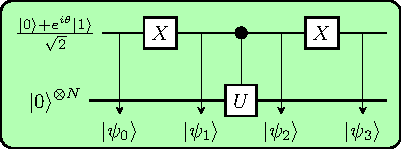
\includegraphics[width=\linewidth]{circuits/circuit1.pdf}
  \caption{Example circuit that measures $e^{i\theta}\sandwich{0}{U}{0}$ for some unitary matrix $U$ and an angle $\theta$}
  \label{fig:circuitreal}
\end{figure}

Circuit \ref{fig:circuitreal} evolves as follows:
\begin{equation*}
	\begin{split}
		\psi_0 
		&= \paren{\frac{\ket 0 + e^{i\theta}\ket 1}{\sqrt 2}}\otimes \ket 0^{\otimes\elec} \\
		\psi_1
		&= \paren{\frac{\ket 1 + e^{i\theta}\ket 0}{\sqrt 2}}\otimes \ket 0^{\otimes\elec} \\
		\psi_2
		&= \frac{\ket 1}{\sqrt 2} \otimes U \ket 0^{\otimes\elec} + \frac{e^{i\theta}}{\sqrt 2}\ket 0 \otimes \ket 0^{\otimes\elec} \\
		\psi_3
		&= \frac{\ket 0}{\sqrt 2} \otimes U \ket 0^{\otimes\elec} + \frac{e^{i\theta}}{\sqrt 2}\ket 1 \otimes \ket 0^{\otimes\elec} \\
		\intertext{\text{We can now change basis to 
		$\ket + = \frac{\ket 0 + \ket 1}{\sqrt 2}$
		and
		$\ket - = \frac{\ket 0 - \ket 1}{\sqrt 2}$:}}
		\psi_3
		&= \frac{\ket + + \ket -}{2} \otimes U \ket 0^{\otimes\elec} + e^{i\theta}\frac{\ket + - \ket -}{2} \otimes \ket 0^{\otimes\elec} \\
		&= \ket + \frac{U + e^{i\theta}I}{2}\ket 0^{\otimes\elec} 
		+ \ket - \frac{U - e^{i\theta}I}{2}\ket 0^{\otimes\elec} 
	\end{split}
\end{equation*}
The probability of measuring $\ket +$ on the first qubit is:
\begin{equation*}
	\begin{split}
		P(\ket +)
		&= \sandwich 0 {
			\paren{\frac{U + e^{i\theta}I}{2}}
			\paren{\frac{U + e^{i\theta}I}{2}}^\dagger
		} 0 \\
		&= \sandwich 0 {
			\paren{\frac{U + e^{i\theta}I}{2}}
			\paren{\frac{U^\dagger + e^{-i\theta}I}{2}}
		} 0 \\
		&= \sandwich 0 {
			\paren{\frac{UU^\dagger + Ue^{-i\theta}I + U^\dagger e^{i\theta}I + I^2}{4}}
		} 0 \\
		&= \sandwich 0 {
			\paren{\frac{Ue^{-i\theta}I + U^\dagger e^{i\theta}I}{4}}
		} 0 
		+ \frac{\sandwich 0 I 0}{2} \\
		&= \sandwich 0 {
			\paren{\frac{Ue^{-i\theta}I + \paren{Ue^{i\theta}I}^\dagger}{4}}
		} 0 
		+ \frac{1}{2} \\
		&= \frac{Re \paren{e^{i\theta}\sandwich 0 { U } 0}}{2}
		+ \frac{1}{2} \\
	\end{split}
\end{equation*}
A more involved circuit that uses this principle comes from Li's paper \shortcite{benjamin}, as shown in figure \ref{fig:circuitbenjamin}

\begin{figure}[hb!]
  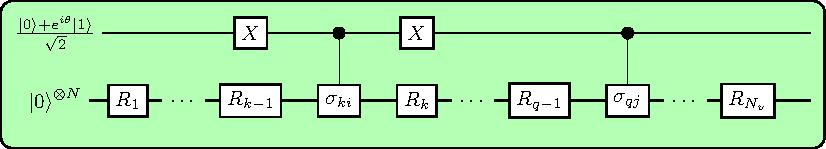
\includegraphics[width=\linewidth]{circuits/circuit2.pdf}
  \caption{Li's circuit to measure $a \cdot Re\paren{e^{i\theta}\sandwich 0 U 0}$, which is then used to calculate $M_{kq}$ for the \gls{tdvp}}
  \label{fig:circuitbenjamin}
\end{figure}
Measuring the first qubit in this circuit yields us:
\begin{equation*}
	\begin{split}
		\ket \phi 
		&= \frac{\ket 0}{\sqrt 2} \otimes R_{N_v} \ldots R_k \cdot \sigma_{ki} \cdot R_{k-1} \ldots R_1 \ket 0^{\otimes \elec}\\
		&\quad + \frac{e^{i\theta}\ket 1}{\sqrt 2} \otimes R_{N_v} \ldots R_q \cdot \sigma_{qj} \cdot R_{q-1} \ldots R_1 \ket 0^{\otimes \elec}\\
		\span\text{We can now use \ref{eq:rki} to simplify our expression:}\\
		&= \frac{\ket 0}{\sqrt 2} \otimes R_{ki} \ket 0^{\otimes \elec}
		+ \frac{e^{i\theta}\ket 1}{\sqrt 2} R_{qj}\ket 0^{\otimes \elec}\\
		\span\text{We can now change basis in our first qubit to
		$\ket + = \frac{\ket 0 + \ket 1}{\sqrt 2}$
		and
		$\ket - = \frac{\ket 0 - \ket 1}{\sqrt 2}$:}\\
		&= \frac{\ket + + \ket -}{2} \otimes R_{ki} \ket 0^{\otimes \elec}
		+ \frac{e^{i\theta}\paren{\ket + - \ket -}}{2} R_{qj}\ket 0^{\otimes \elec}\\
		&= \ket + \otimes \frac{R_{ki} + e^{i\theta}R_{qj}}{2} \ket 0^{\otimes \elec}
		 + \ket - \otimes \frac{R_{ki} - e^{i\theta}R_{qj}}{2} \ket 0^{\otimes \elec}
	\end{split}
\end{equation*}
The probability of measuring $\ket +$ on the first qubit is:
\begin{equation*}
	\begin{split}
		P(\ket +)
		&= \sandwich 0 {
			\frac{1}{2}\paren{R_{ki} + e^{i\theta} R_{qj}}
			\frac{1}{2}\paren{R_{ki} + e^{i\theta} R_{qj}}^{\dagger}
		} 0 \\
		&= \frac 1 4 \sandwich 0 {
			\paren{R_{ki} + e^{i\theta} R_{qj}}
			\paren{R_{ki}^\dagger + e^{-i\theta} R_{qj}^{\dagger}}
		} 0 \\
		&= \frac 1 4 \sandwich 0 {
			R_{ki}R_{ki}^\dagger + e^{-i\theta} R_{ki}R_{qj}^{\dagger} 
			+ e^{i\theta} R_{qj}R_{ki}^\dagger + R_{qj}R_{qj}^\dagger
		} 0 \\
		&= \frac 1 4 \sandwich 0 {
			e^{-i\theta} R_{ki}R_{qj}^{\dagger} + \paren{e^{-i\theta} R_{ki}R_{qj}^\dagger}^\dagger
		} 0 
			+ \frac{\sandwich 0 I 0}{2}\\
		&= \frac 1 2 Re\paren{e^{i\theta}\sandwich 0 {
			 R_{ki}R_{qj}^{\dagger}
	} 0 }
			+ \frac{1}{2}\\
	\end{split}
\end{equation*}
The probability of measuring $\ket -$ on the first qubit is then:
\begin{equation*}
	\begin{split}
		P(\ket -)
		= \frac 1 2 - \frac 1 2 Re\paren{e^{i\theta}\sandwich 0 {
			 R_{ki}R_{qj}^{\dagger}
	} 0 }
	\end{split}
\end{equation*}
The average measurement of this circuit is then $Avg = P(\ket +) \cdot 1 + P(\ket -) \cdot (-1) = Re\paren{e^{i\theta}\sandwich 0 {R_{ki}R_{qj}^{\dagger}} 0}$ since the eigenvalue of $\ket +$ is 1 and the eigenvalue of $\ket -$ is -1.

Taking $a_{kiqj} = \abs{if_{k, i}^*f_{q, j}}, \theta = \arg \paren{if_{k, i}^*f_{q, j}}$ and referring back to \ref{eq:benjamin}:
\begin{equation*}
	\begin{split}
		\sum_{i, j \in P} a_{kiqj} \cdot Avg_{kiqj} 
		&= \sum_{i, j \in P} a_{kiqj}\cdot Re\paren{e^{i\theta}\sandwich 0 {R_{ki}R_{qj}^{\dagger}} 0}\\
		&= \sum_{i, j \in P} a_{kiqj}\cdot Re\paren{\frac{if_{k, i}^*f_{q, j}}{\abs{if_{k, i}^*f_{q, j}}}\sandwich 0 {R_{ki}R_{qj}^{\dagger}} 0}\\
		&= \sum_{i, j \in P} \frac{a_{kiqj}}{\abs{if_{k, i}^*f_{q, j}}} Re\paren{if_{k, i}^*f_{q, j}\sandwich 0 {R_{ki}R_{qj}^{\dagger}} 0}\\
		&= \sum_{i, j \in P} 2 Re\paren{if_{k, i}^*f_{q, j}\sandwich 0 {R_{ki}R_{qj}^{\dagger}} 0}\\
		&= \sum_{i, j \in P} 
		\left [if_{k, i}^*f_{q, j}\sandwich 0 {R_{ki}R_{qj}^{\dagger}} 0 +
		\paren{if_{k, i}^*f_{q, j}\sandwich 0 {R_{ki}R_{qj}^{\dagger}} 0}^* \right ] = M_{k, q}\\
	\end{split}
\end{equation*}
Using our evaluation of $\ket\Psi$ in terms of $\rho_\ind 0, \rho_\ind 1, \omega_\ind 0, \omega_\ind 1$, we get the following for R, using \ref{eq:udecomposition}:
\begin{align*}
	\ket\Psi &= R\ket 0 
	= \sum_{\ind 0} \paren{
		u_{\lambda_{\ind 0}} \otimes \ket{\ind 0} \bra{\ind 0} }\ket 0 \\
	&= \sum_{\ind 0} \paren{
		R_z(\omega_{\ind 0}) R_y(2\rho_\ind 0) R_z(-\omega_\ind 0) \otimes \ket{\ind 0} \bra{\ind 0}} \ket 0
\end{align*}

We can rewrite $R$ as:
\begin{align*}
	R 
	&= \sum_{\ind 0} 
		R_z(\omega_{\ind 0}) R_y(2\rho_\ind 0) R_z(-\omega_\ind 0) \otimes \ket{\ind 0} \bra{\ind 0}
	=\prod_{k=N_v}^1 R_k(\lambda_k)
\end{align*}

We can now use the $R_k$ to find our $f_{k, i}$ via \ref{eq:r_to_f}. Finally, we use the values obtained to obtain the gates used in, for example, circuit \ref{fig:circuit}.

%-------------------------------------------------------------------------------------

\chapter{\textbf{Initial Results and Research Directions}}\label{chap:results}

Using Fukutome's \shortcite{fukutome} unitary approach to the \gls{hf} method together with some other approximations, we've obtained a reference wavefunction $\ket \Psi(\bm \omega, \bm \rho) = \hat U\ket 0$ that depends on vectors of real rotation angles $\bm \omega$ and $\bm \rho$.

Next, we've solved the Euler-Lagrange differential equation system related to that wavefunction to get an algebraic result for the matrices in our system.
We've then decomposed $\hat U$ into a product of matrices that depend on a single variable $\hat U = \prod_{\ind 0} R(\lambda_{\ind 0})$.

We've then adapted the construction of the circuit from Li \shortcite{benjamin} to cater to our reduced set of variables and developed circuits to calculate each of the elements of the matrices $\bm M$ and $\bm V$ at each step of the \gls{tdvp} so we could solve the differential equations $\sum_q \bm M_{k,q}\dot{\lambda}_q = V_k$ and simulate the state of our system. One such circuit built using qiskit in python is the one on figure \ref{fig:circuit}. Computational results confirming the research are in progress.
\begin{figure}[hb!]
  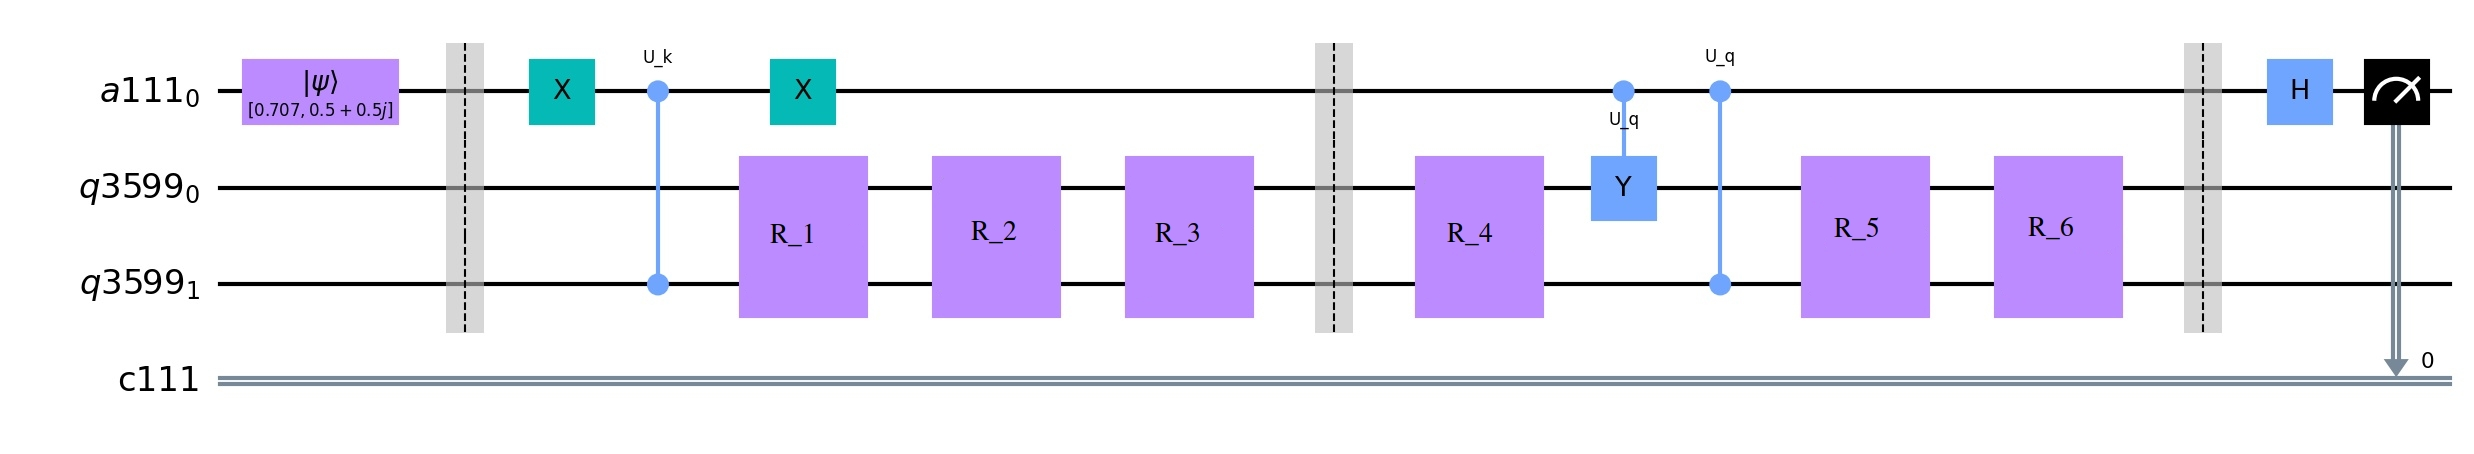
\includegraphics[width=\linewidth]{img/circuit.jpg}
  \caption{Circuit for $k = 1, q = 4, \sigma_{1, iz}, \sigma_{4, yi}, \elec = 2, \orb = 4$}
  \label{fig:circuit}
\end{figure}

The theoretical algebraic derivations for the low-dimension cases for this research has already been laid out and it looks promising for higher dimensions systems, so this could be scaled for the dynamical modeling of bigger systems than the ones provided here.
With equations for the wavefunction in hand, a circuit can be built to obtain matrices $\bm M$ and $\bm V$ needed to solve the system of Euler-Lagrange equations and accelerate the \gls{tdvp}.

\begin{figure}[h!]
	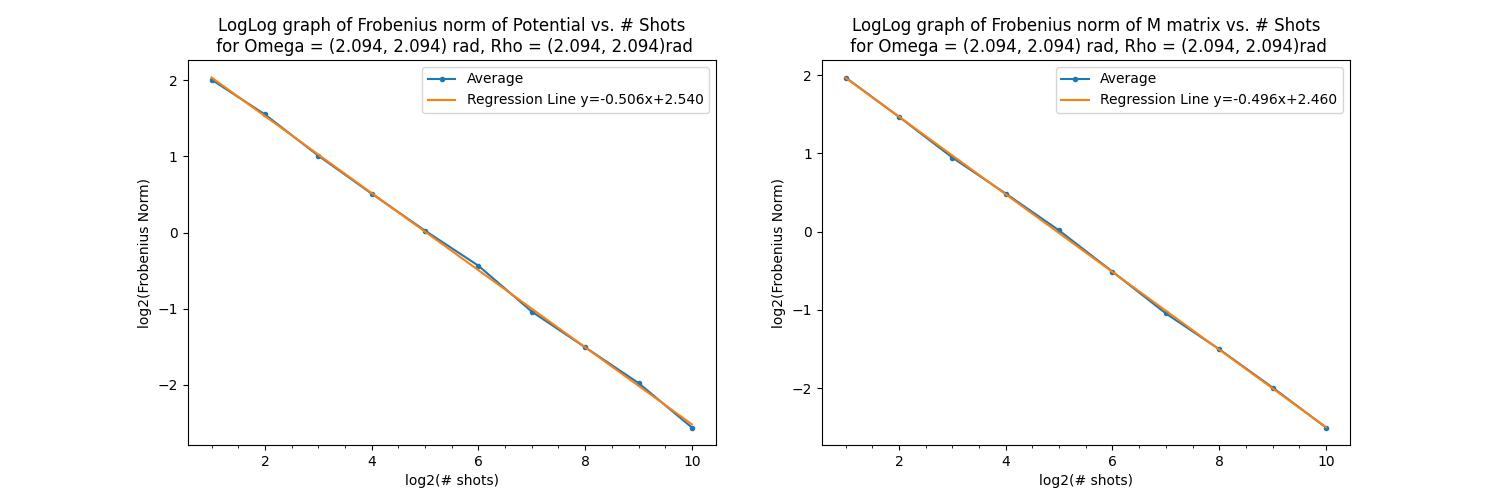
\includegraphics[width=\linewidth]{img/M&V Graph.jpg}
  \caption{Loglog graph of error vs number of shots for a hydrogen molecule}
  \label{fig:2derrorgraph}
\end{figure}

Current results in our simulations of a hydrogen atom as well as a hydrogen molecule suggest that the error $E$ in the approximation for the elements of both the potential matrix $\bm V$ and the matrix $\bm M$ follow the same relationship with the number of shots $S$ in the circuits, as seen in \ref{fig:2derrorgraph}:

\begin{equation*}
	\begin{split}
		\log E &= -\frac 1 2 \log S + c \\
		E &= \frac 1 {\sqrt{S}} + c \\
	\end{split}
\end{equation*}

Which means the assymptotical behaviour of our error is $\mathcal O(S^{-\frac 1 2})$

Further research could be made using the non-unitary representation for $\hat U$ in combination with \gls{lcu} to allow for \gls{qc} in the non-unitary case or even different formulations for the wavefunction in place of \gls{hf}.

%%%%%%%%%%%%%%%%%%%%%%%%%%%%%%%%%%%%%%%%%%%%%%%%%%%%%%%%%%%%%%%%%%%%%%%%%%%%%%%%%%%%%%%%%
%%%%%%%%%%%%%%%%%%%%%%%%%%%%%%%%%%%%%%%%%%%%%%%%%%%%%%%%%%%%%%%%%%%%%%%%%%%%%%%%%%%%%%%%%
%%% 							END OF SECOND CHAPTER								  %%%
%%%%%%%%%%%%%%%%%%%%%%%%%%%%%%%%%%%%%%%%%%%%%%%%%%%%%%%%%%%%%%%%%%%%%%%%%%%%%%%%%%%%%%%%%
%%%%%%%%%%%%%%%%%%%%%%%%%%%%%%%%%%%%%%%%%%%%%%%%%%%%%%%%%%%%%%%%%%%%%%%%%%%%%%%%%%%%%%%%%

%TODO: new document or added section
%\chapter{\textbf{Career goals}}
%%%%%%%%%%%%%%%%%%%%%%%%%%%%%%%%%%%%%%%%%%%%%%
%Backmatter -- Bibliography, appendices, etc.%
%%%%%%%%%%%%%%%%%%%%%%%%%%%%%%%%%%%%%%%%%%%%%%
\backmatter


%%%%%%%%%%%%%%%%%%%%%%%%%%%%%%%%%%%%%%%%%%%%%%%%%%%%%%%%
%Bibliography:  Use BibTeX 							   %
%%%%%%%%%%%%%%%%%%%%%%%%%%%%%%%%%%%%%%%%%%%%%%%%%%%%%%%%
\bibliographystyle{chicago}
\addcontentsline{toc}{chapter}{\textbf{References}}
\bibliography{aux/refs}

\glsaddall

%\setlength{\glsdescwidth}{0.5\linewidth}
%\setlength{\glspagelistwidth}{0.1\linewidth}
\printnoidxglossary[type=acronym,sort=letter]
%\printnoidxglossary[type=symbols,sort=letter]

\end{document}
